% !TeX spellcheck = en_US
\documentclass[
english,
openany,
draft = false,
twoside = true,
fleqn
]{scrbook}
\usepackage{learning-notes}

\author{Huu Duc Nguyen}
\authordegreefront{}
\authordegreeback{ M.Sc.}
\subject{AI}
\title{AI Notes}
\date{29 February 2022}

\begin{document}
\setlength{\abovedisplayskip}{3pt}
\setlength{\belowdisplayskip}{3pt}

\frontmatter
\TitlePage
\tableofcontents

\mainmatter
% !TeX spellcheck = en_GB
\chapter*{Abbreviations}
\addcontentsline{toc}{chapter}{Abbreviations}

\begin{acronym}[LONGEST]
\acro{AI}{Artificial Intelligence}
\acro{AGI}{Artificial General Intelligence}
\acro{ML}{Machine Learning}
\acro{DL}{Deep Learning}
\acro{CS}{Computer Science}
\acro{CV}{Computer Vision}
\acro{RL}{Reinforcement Learning}
\acro{NLP}{Natural Language Processing}
\acro{GPU}{Graphics Processing Unit}
\acro{CPU}{Central Processing Unit}

% Conferences
\acro{ICML}{\href{https://icml.cc/}{International Conference on Machine Learning}}

\acro{prob}[prob.]{probability}
\acro{param}[params.]{parameters}
\acro{algor}[algor.]{algorithms}
\acro{info}[info.]{information}
\acro{aka}[a.k.a.]{also known as}
\acro{wrt}[w.r.t.]{with regard to}
\acro{no}[no.]{number of}
\acro{func}[func.]{function}
\acro{vs}[vs.]{versus}
\acro{freq}[freq.]{frequency}
\acro{st}[s.t.]{subject to}

\acro{iid}[i.i.d.]{independent \& identically distributed}
\acro{LSI}{linear shift invariant}
\acro{pdf}[pdf.]{Probability Density Function}
\acro{MLE}{Maximum Likelihood Estimation}
\acro{MAP}{Maximum A Posteriori}
\acro{MoG}{Mixture of Gaussians}
\acro{SVM}{State Vector Machine}

% Gradient descent
\acro{GD}{Gradient Descent}
\acro{SGD}{Stochastic Gradient Descent}
\acro{nag}[NAG]{Nestorov Accelerated Gradient}
\acro{rmsprop}[RMSprop]{Root mean squared prop}
\acro{adam}[Adam]{Adaptive moment estimation}

\acro{SVD}{Singular Value Decomposition}
\acro{PCA}{Principal Component Analysis}
\acro{LDA}{Linear Discriminant Analysis}
\acro{KL}[KL]{Kullback–Leibler}
\acro{IG}{Information Gain}

% Mathematics & Optimization
\acro{KKT}{Karush-Kuhn-Tucker}
\acro{RBF}{Radial basic function}
\acro{iff}[i.f.f.]{if and only if}
\acro{LP}{Linear Programming}
\acro{QP}{Quadratic Programming}
\acro{LQR}{Linear Quadratic Regulator}
\acro{iLQR}{Iterative Linear Quadratic Regulator}
\acro{MPC}{Model Predictive Control}
\acro{FLM}{Fitted Local Model}
\acro{FFT}{Fast Fourier Transform}

% Neural-network-related term
\acro{MLP}{Multi-Layer Perceptron}
\acro{relu}[ReLU]{Rectified Linear Unit}
\acro{BPTT}{Backpropagation through time}
\acro{RNN}{Recurrent Neural Network}
\acro{LSTM}{Long short-term memory}
\acro{CNN}{Convolutional Neural Network}
\acro{GNN}{Graph Neural Network}
\acro{CONV}{Convolutional}
\acro{FC}{Fully Connected}
\acro{VAE}{Variational Auto-Encoders}
\acro{GAN}{Generative Adversarial Network}
\acro{DCGAN}{Deep Convolutional Generative Adversarial Network}
\acro{CGAN}{Conditional Generative Adversarial Network}
\acro{SRGAN}{Super Resolution Generative Adversarial Network}
\acro{ESRGAN}{Enhanced Super Resolution Generative Adversarial Network}
\acro{ResNet}{Residual Network}
\acro{BatchNorm}{Batch Normalization}
\acro{IN}{Instance Normalization}
\acro{AdaIN}{Adaptive Instance Normalization}
\acro{NAS}{Neural Architecture Search}

% Robotics
\acro{dof}[DOF]{degrees of freedom}
\acro{ee}[EE]{end-effector}
\acro{DH}[D-H]{Denavit–Hartenberg}

% Probabilistic Robotics
\acro{KF}{Kalman Filter}
\acro{EKF}{Extended Kalman Filter}
\acro{IF}{Information Filter}
\acro{EIF}{Extended Information Filter}
\acro{MHEKF}{Multi-Hypothesis Extended Kalman Filter}

% Reinforcement learning related
\acro{HMM}{Hidden Markov Model}
\acro{MDP}{Markov Decision Process}
\acro{POMDP}{Partially Observable Markov Decision Process}
\acro{TSP}{Travelling Salesman Problem}
\acro{A3C}{Asynchronous advantage actor-critic}
\acro{SAC}{Soft actor-critic}
\acro{DQN}{Deep Q-learning}
\acro{DDP}{Differential Dynamic Programming}
\acro{dagger}[DAgger]{Dataset Aggregation}
\acro{CEM}{Cross-entropy Method}
\acro{MCTS}{Monte-Carlo Tree Search}
\acro{MBA}{Model-based Acceleration}
\acro{MVE}{Model-based Value Expansion}
\acro{MBPO}{Model-based Policy Optimization}
\acro{UCB}{Upper Confidence Bounce}
\acro{PAC}{Probably Approximately Correct}
\acro{CQL}{Conservative Q-learning}
\acro{MOPO}{Model-Based Offline Policy Optimization}
\acro{IRL}{Inverse Reinforcement Learning}
\acro{MaxEnt}{Maximum Entropy}
\acro{MAML}{Model-Agnostic Meta-Learning}
\acro{OPE}{Off-policy evaluation}
\acro{LSTD}{Least-squares temporal difference}
\acro{LSPI}{Least-squares policy iteration}

% Computer vision related
\acro{DPM}{Deformable Part Model}
\acro{HOG}{Histogram of Oriented Gradients}
\acro{SSIM}{Structural Similarity Index}
\acro{SRCNN}{Super Resolution Convolutional Neural Network}
\acro{PPL}{Perceptual path length}
\acro{FID}{Fréchet inception distance}

% Psychology related
\acro{US}{unconditioned stimuli}
\acro{UR}{unconditioned response}
\acro{CS}{conditioned stimuli}
\acro{CR}{conditioned response}
% Neuroscience related
\acro{CNS}{central nervous system}
\acro{PNS}{peripheral nervous system}
\acro{EEG}{Electroencephalography}
\acro{fMRI}{Functional Magnetic Resonance Imaging}
\acro{ECoG}{Electrocorticography}
\acro{LFP}{Local Field Potentials}
\acro{BCI}{Brain-Computer Interface}
\acro{BMI}{Brain Machine Interface}
\acro{NMP}{neuromotor prostheses}
\acro{PSD}{Power Spectral Density}

\end{acronym}
% !TeX spellcheck = en_US
\chapter{Introduction}

\ac{AI} is the study field that leverages the ability of machines to mimic the problem-solving skill of human. It lies in the core of countless novel applications in real life, self-driving cars, virtual assistant, face recognition, \etc. \ac{ML} is a sub-field of \ac{CS} and \ac{AI}, that “gives computers the ability to learn without being explicitly programmed” (\href{https://en.wikipedia.org/wiki/Machine_learning}{Wikipedia}). As a great amount of collected data and powerful computational hardware arise, \ac{DL} is then a subset of \ac{ML} (\figref{fig:relation-ai-ml-dl}). Advanced applications which relate to \ac{NLP}, \ac{CV}, robotic learning, \etc, are with in this \ac{DL} subset.
\begin{figure}[hbt!]
	\centering
	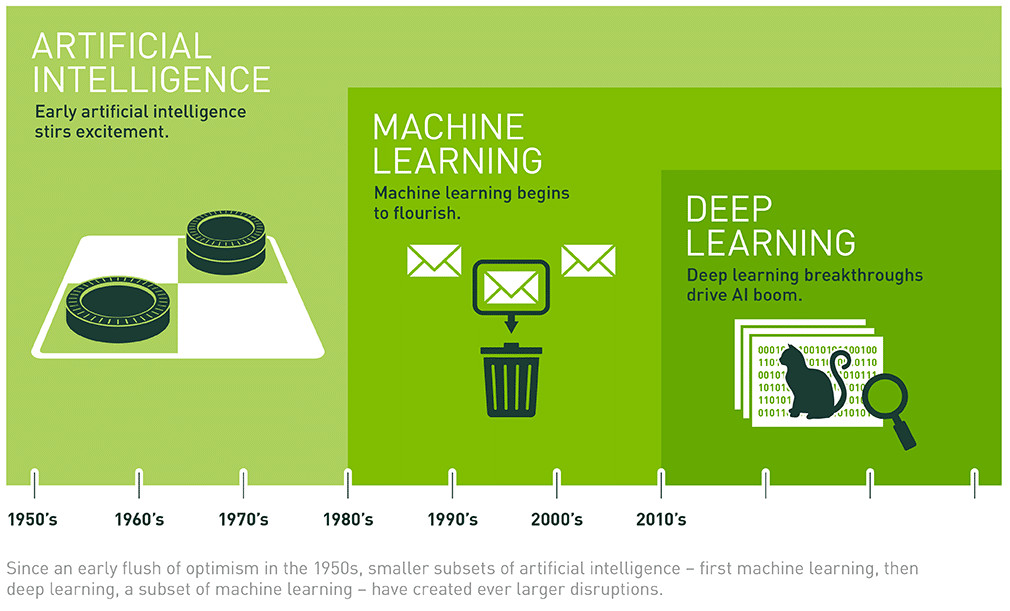
\includegraphics[width=1\textwidth]{nvidia-ai-ml-dl.jpg}
	\caption{The relation between \ac{AI}, \ac{ML} and \ac{DL} (\href{https://developer.nvidia.com/deep-learning}{src}).}
	\label{fig:relation-ai-ml-dl}
\end{figure}

\todo{The structure of the notes}\\
It's important to understand that there are more to \ac{AI} and \ac{ML} than just neural networks. In the end, to create a meaningful and working neural network, I believe one should have strong background in the basics of \ac{ML} as well. Henceforth, I keep record of what I have learnt in the whole \ac{AI} field. The structure of the notes is as follows:
\begin{itemize}
	\item \charef{cha:probabilities} introduces the mathematics background on probabilities, matrix.
	\item \todo{chapter 3} explain basic concepts, the branching of different classes in \ac{ML}. Later chapters presents each smaller branches.
\end{itemize}
% !TeX spellcheck = en_US
\chapter{Overview of Machine Learning}
\label{cha:overview-ml}

A machine learning algorithm is an algorithm that has the ability to \textit{learn} from the data. A computer program is said to \textbf{learn}, if its performance at tasks in $T$, measured by $P$, improves with experience $E$ (in which the experience is equivalent to the data). \cite{goodfellow2016deep}

\section{Task $T$}
A \textit{task} is usually described by how the \ac{ML} model process a single \textit{data point}. This section presents some common \ac{ML} tasks. \cite{vu2018mlcb}

\subsection{Classification}
The task is to specify a label for the given data point. The labels are usually members of a list.

\Eg, in the problem of digit classification, the data point is images of hand-written numbers. The data set comes with their labels as well. The task is then, given a unseen image, the model would be able to tell which number is in that image. In this problem, there are 10 possible labels, \ie, $0, 1, \dots, 9$.

\subsection{Regression}
If the desired output is a real value, instead of a label in a list, then it's a regression problem. \Eg:
\begin{itemize}
	\item with an image as the input data, the model predicts the age of the person
	\item given a feature vector, the model generates an image
\end{itemize}

\subsection{Clustering}
This is the task of grouping relevant data points based on some relationship between them.

\Eg, find the pattern in customer shopping behaviors.

\subsection{Others}
Some worth-mentioning tasks:
\begin{itemize}
	\item Recommendation System
	\item Machine Translation
	\item Completion
	\item Ranking
	\item Information Retrieval
	\item Denoising
\end{itemize}

\section{Performance $P$}
Usually, the dataset is divided into \textit{training set} and \textit{test set}. The model uses the training set to tune \ update the model \ac{param} and the test set to examine the performance.

\textit{Online training} is the approach when new data will continuously arise and introduce for the model to learn. \Eg in \ac{RL}. \textit{Offline training} is the opposite, the model learns from the a fixed training set.

\section{Experience $E$}
\subsection{Supervised Learning}
Supervised Learning is the approach that predict the outputs of new data points based on pairs of known inputs and outputs. This is the most common type of \ac{ML} \ac{algor}.
\subsection{Unsupervised Learning}
On the opposite, with unsupervised Learning, there is no known output, just inputs. Unsupervised Learning \ac{algor} will carry on some tasks based on the characteristics of the dataset, \eg clustering, dimension reduction.

\section{Model Parameters and Loss Function}
\label{sec:model-param-loss}
Each \ac{ML} model is described by a set of model \ac{param}. \Eg, in the problem of finding a line passing through points in the 2D plane, the model \ac{param} are $a, b$ in the line equation $y=ax+b$. The of training aim is to find the model \ac{param} that leads to the best performance. For classification problems, it means having the least number of incorrect classified data points. For regression problems, it means having the smallest difference with the actual output. It is then equivalent to having a optimization problem, in which we try to minimize a loss/cost function.
% !TeX spellcheck = en_US
\chapter{Probabilities}
\label{cha:probabilities}

\section{Definitions}
\label{sec:prob-defs}

\subsection{Basic Definitions}
\begin{itemize}
	\item If $x$ is discrete: $\underset{x}{\sum} p(x) = 1$ with $\forall$ $0 \leq p(x) \leq 1$
	\item If $x$ is continuous: $\displaystyle \int p(x) \,dx = 1 \Rightarrow \exists$ a \textbf{\ac{pdf}}\\
	$p(x)$ can take any positive value, as long as \(\displaystyle \int p(x) \,dx = 1\)\\
	\todo{Add image}\\
	\note: theoretically $p(x) = 0, \forall x$
	\item Common types
	\begin{align*}
		& \text{Joint probability:} 		&& p(x_i, y_i) 	&& \left(= p(X=x_i, Y=y_i)\right) \\
		& \text{Marginal probability:} 		&& p(x_i) 		&& \left(= p(X=x_i)\right) \\
		& \text{Conditional probability:} 	&& p(y_i | x_i) && \left(= p(Y=y_i|X=x_i)\right)
	\end{align*}	
	\item Sum rule: $\displaystyle \sum$ joint \ac{prob} = marginal \ac{prob}\\
	$\Rightarrow$ Marginalization	
	\begin{itemize}
		\item discrete variable: $\displaystyle p(x)=\underset{y}{\sum} p(x, y)$
		\item continuous variable: $\displaystyle p(x) = \int p(x,y) dy$
	\end{itemize}
	\item Product rule: Product of marginal \ac{prob} and conditional \ac{prob} = joint \ac{prob}
\end{itemize}

\subsection{Independence and Variability}
\begin{itemize}
	\item Independence. \Eg: $x, y$ are independent, then
	\[\begin{cases}
		p(x|y) = p(x)\\
		p(y|x) = p(y)
	\end{cases}
	\iff p(x,y) = p(x).p(y)\]
	
	\item Variability
	\begin{itemize}
		\item variance:\\ $var \left[f\right] = \expectation{\left(f(x)-\expectation{f(x)}\right)^2} = \expectation{f(x)^2} - \expectation{f(x)}^2$
		\item covariance:\\ $cov \left[x, y\right] = \mathbb{E}_{x,y}\left[xy\right] - \expectation{x}.\expectation{y} = \mathbb{E}_{x,y}\left[xy^T\right] - \expectation{x}.\expectation{y^T}$
		\item covariance matrix
	\end{itemize}
\end{itemize}

\subsection{Bayes Rule}
\label{subsec:bayes-rule}
\begin{align*}
	& p(x_i|y_i).p(y_i) = p(y_i|x_i).p(x_i) = p(x_i, y_i) \\
	\Rightarrow\; &p(y_i|x_i) = \frac{p(x_i|y_i).p(y_i)}{p(x_i)} = \frac{p(x_i|y_i).p(y_i)}{\underset{y}{\sum} p(x_i|y_i).p(y_i)}
\end{align*}
$\Rightarrow$ the \hlb{Bayes equation}:\\~\\
\hlre{posterior = \frac{likelihood \times prior}{normalization~factor}}

\subsection{Expectation}
\label{subsec:expectation}
\begin{align*}
	& \text{For variable $x$:} && \expectation{x} = \underset{x}{\sum}x.p(x) && \left( = \int x.p(x)dx \right)\\
	& \text{For function $f(\cdot)$:} && \expectation{f(x)} = \underset{x}{\sum}f(x).p(x) && \left( = \int f(x).p(x)dx \right)
\end{align*}

\section{Types of Probability Distributions}
Reference source: \href{https://machinelearningcoban.com/2017/07/09/prob/}{machinelearningcoban.com}.
\subsection{Bernoulli Distribution}
Bernoulli Distribution is a distribution to describe binary discrete variables. It's the case that the variable can only take value in 2 classes $x \in \{0,1\}$. \Eg, the probability of throwing a coin. The Bernoulli distribution is defined with parameter $\lambda \in[0,1]$:
\begin{equation}
	p(x) = \text{Bern}_x[\lambda] = \begin{cases}
		p(x=1) = \lambda\\
		p(x=0) = 1-\lambda
	\end{cases}
\end{equation}
In short form, the above equation can be combined into one:
\begin{equation}
	p(x) = \lambda^x(1-\lambda)^{(1-x)} \Rightarrow
	\begin{cases}
		p(0) = \lambda^0 (1-\lambda)^1 = 1-\lambda \\
		p(1) = \lambda^1 (1-\lambda)^0 = \lambda \\
	\end{cases}
\end{equation}

\subsection{Categorical Distribution}
\label{subsec:categorical-distribution}
\textit{Categorical Distribution} is the generalization of \textit{Bernoulli Distribution}, in case there are $K$ classes for the discrete variable $x \in \{ 1, 2, \dots, K\}$. Accordingly, there will be $K$ parameters to describe this \ac{pdf}: $\lambda = [\lambda_1, \lambda_2, \dots, \lambda_K]$, with $\lambda_k \geq 0$ and $\sum \lambda_k = 1$. Each $\lambda_k$ represents the probability to take the output $k$: $p(x = k) = \lambda_k$. In short: $p(x) = \text{Cat}_x [\lambda]$.

Another common way to represent the output is the one-hot vector, $\mathbf{x} \in \{\mathbf{e}_1, \mathbf{e}_2, \dots, \mathbf{e}_K\}$ with $\mathbf{e}_k$ is the $k$-unit vector, which has all 0-element, except the $k$-element equal to 1. \Eg, given 3 classes: $\textbf{e}_1 = [1, 0, 0]^T, \textbf{e}_2 = [0, 1, 0]^T, \textbf{e}_3 = [0, 0, 1]^T$. We will then have:
\begin{equation}
	p(\mathbf{x} = \mathbf{e}_k) = \prod_{j=1}^K \lambda_j^{x_j} = \lambda_k
\end{equation}
because for $\textbf{x}=\textbf{e}_k$, only $x_k=1$, while $x_j = 0, \forall j\neq k$.

\subsection{Univariate Normal Distribution}
Univariate Normal Distribution is also known as the Gaussian distribution. For single dimension data (in 1D): $x \in (-\infty, \infty)$, the mean $\mu \in \mathbb{R}$, and the variance $\sigma^2$ with $\sigma \in \mathbb{R}$.
\begin{equation}
	p(x) = \text{Norm}_x\left[\mu, \sigma^2\right] = \mathcal{N}(\mu, \sigma^2) = \frac{1}{\sqrt{2\pi\sigma^2}}.\text{exp}\left(-\frac{(x-\mu)^2}{2\sigma^2}\right)
\end{equation}
\note
\begin{itemize}
	\item \hlr{Marginals \ac{prob} of Gaussian are again Gaussian.}
	\item When estimating the \ac{param} of a Gaussian, beware the underestimation problem.
	\begin{align*}
		\expectation{\mu_{ML}} &= \mu \\
		\expectation{\sigma^2_{ML}} &= \left(\frac{N-1}{N}\right)\sigma^2 \\
		\Rightarrow \overset{\sim}{\sigma}^2 &= \left(\frac{N}{N-1}\right)\sigma^2_{ML} = \frac{1}{N-1} \sum_{n=1}^{N} (x_n-\hat{\mu})^2
	\end{align*}
\end{itemize}
\begin{figure}[hbt!]
	\centering
	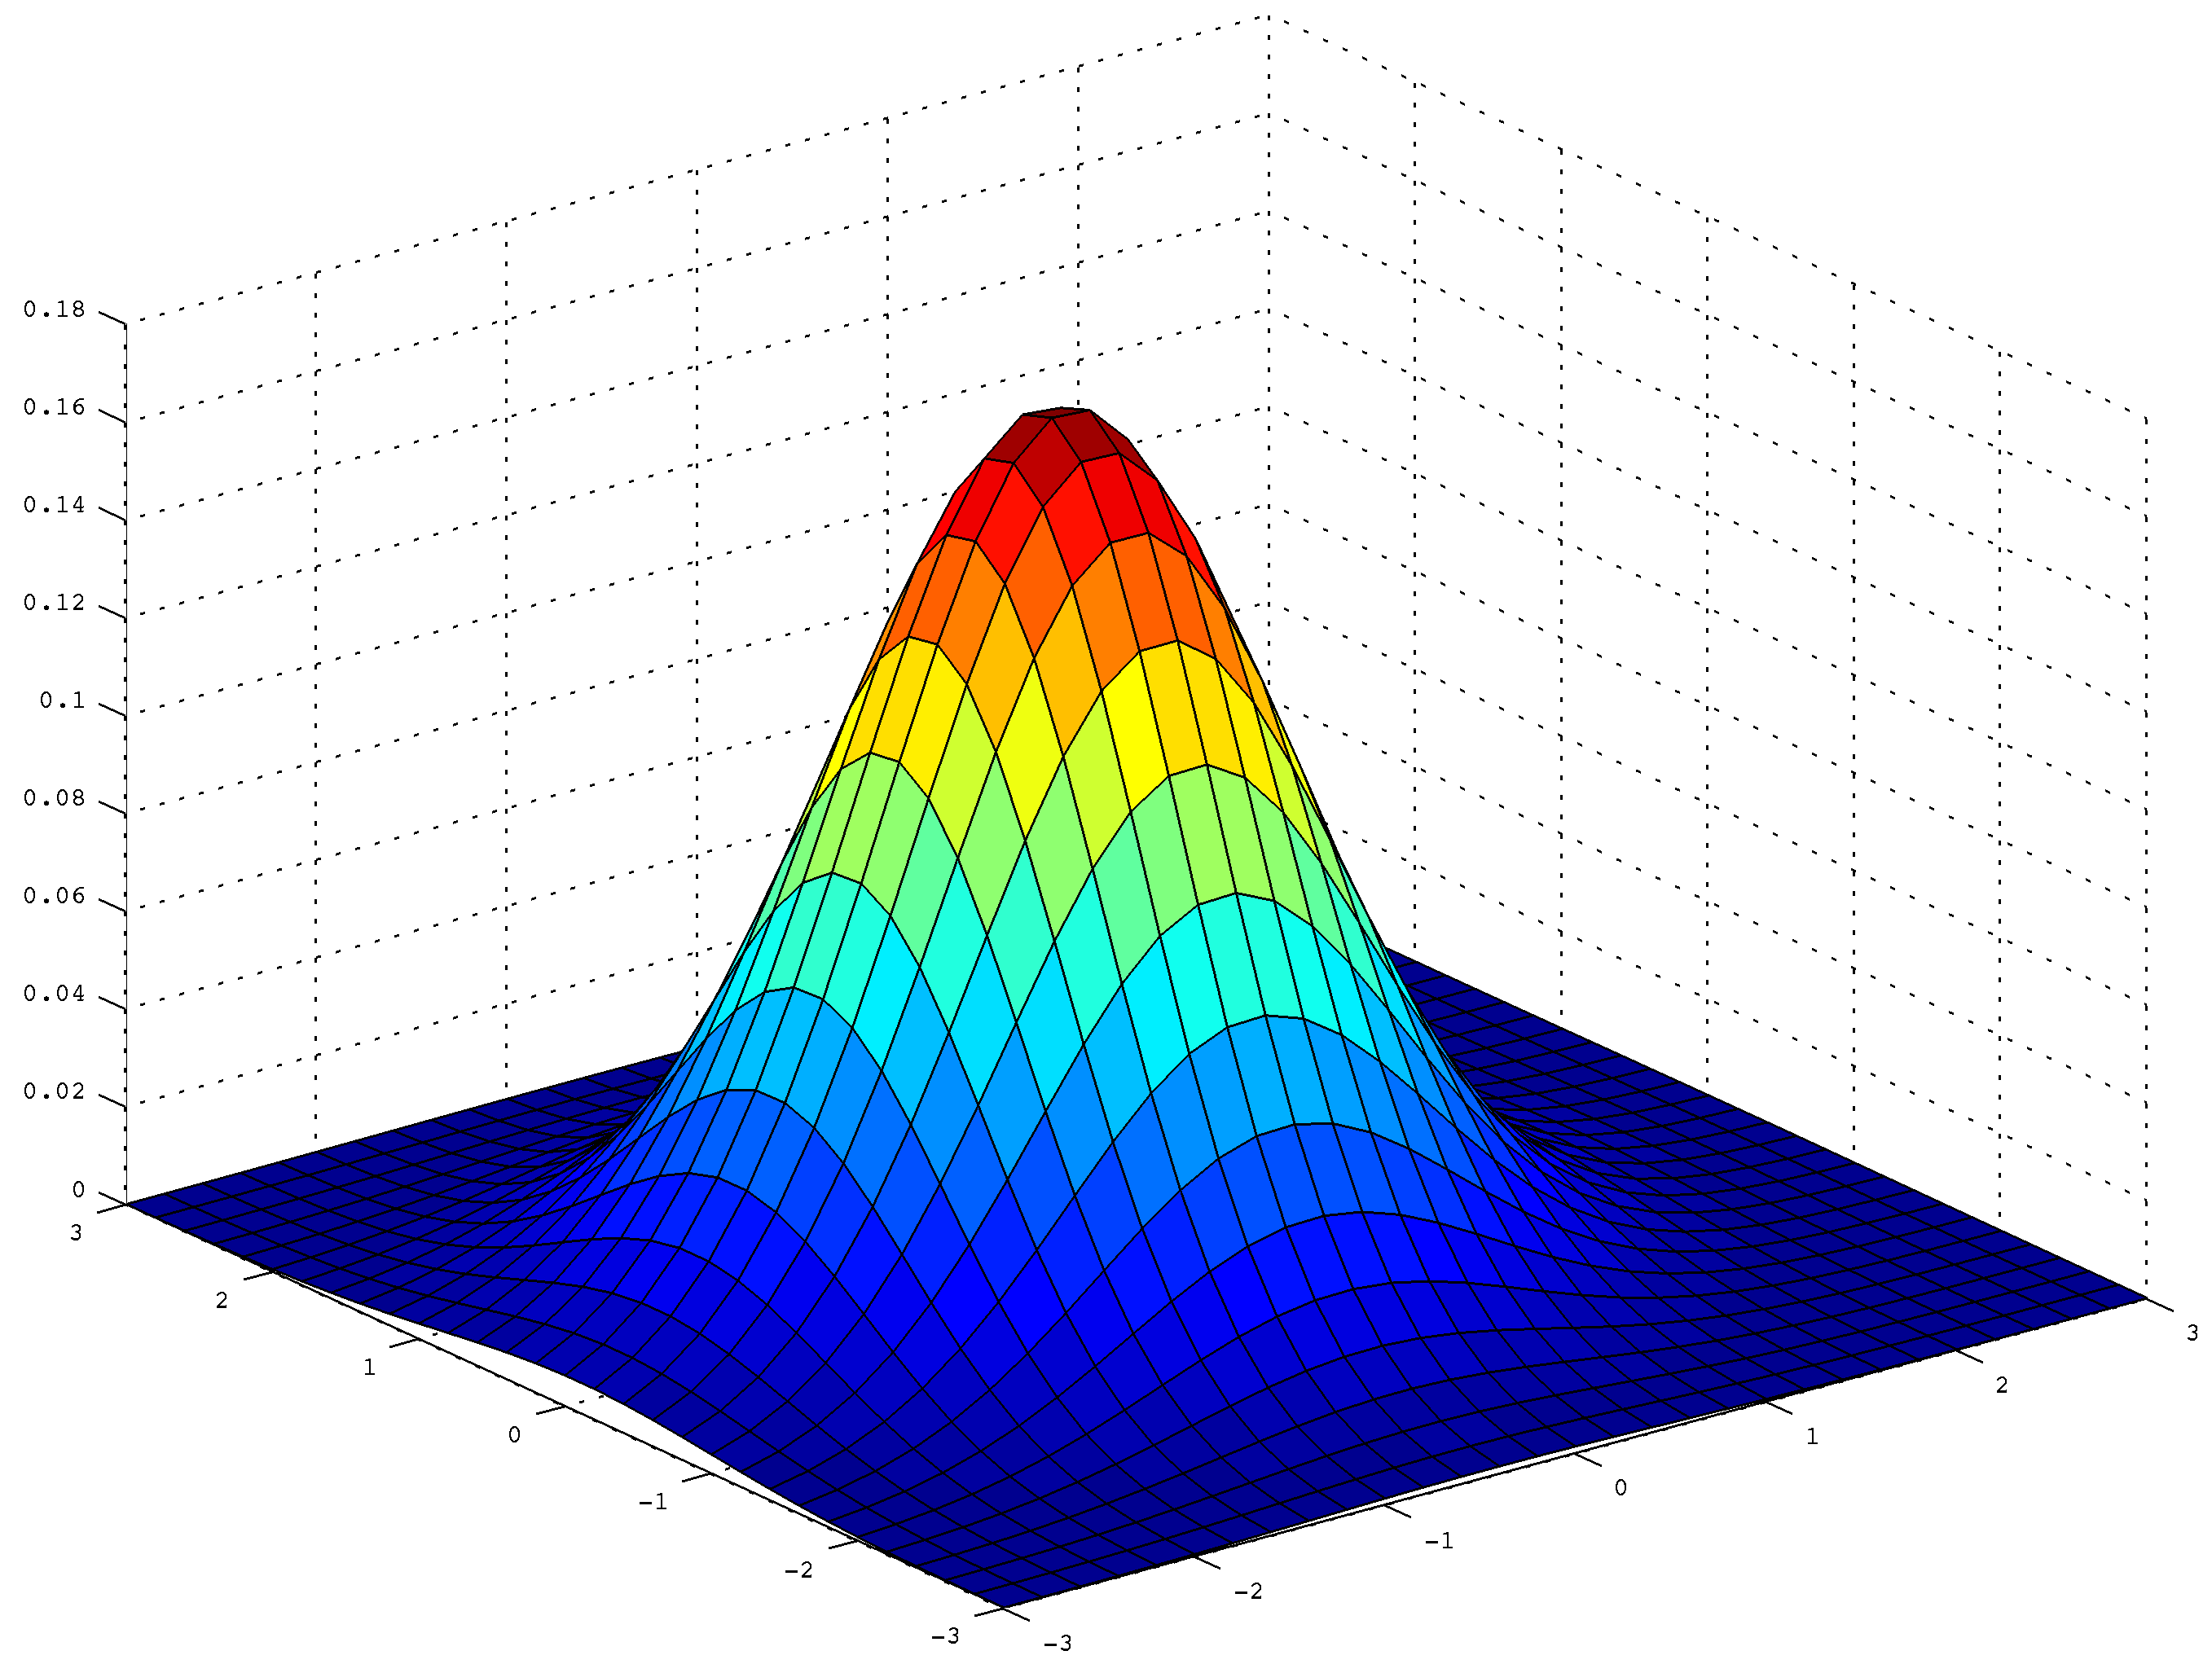
\includegraphics[width=0.7\textwidth]{gaussian-pdf.png}
	\caption{Bivariate Gaussian distribution (\href{https://stats.stackexchange.com/questions/102632/plot-two-dimensional-gaussian-density-function-in-matlab}{src}).}
	\label{fig:relation-ai-ml-dl}
\end{figure}

\subsection{Multivariate Normal Distribution}
\textit{Multivariate Normal Distribution} is the extension of \textit{Univariate Normal Distribution} to multi-dimensional data: $\textbf{x}, \boldsymbol{\mu} \in \mathbb{R}^D, \sigma^2 \Rightarrow \Sigma \in \mathbb{S}^D_{++}$ ($\mathbb{S}^D_{++}$ is the set of positive definite symmetric matrix)
\begin{equation}
	p(x) = \text{Norm}_x [\boldsymbol{\mu}, \Sigma] = \mathcal{N}(\boldsymbol{\mu}, \Sigma) = \frac{1}{2\pi^{D/2}| \Sigma|^{\frac{1}{2}}} . \text{exp} \left( -\frac{1}{2} {(\textbf{x} - \boldsymbol{\mu})^T \Sigma^{-1} (\textbf{x} - \boldsymbol{\mu})} \right)
\end{equation}

\subsection{Beta Distribution}
This distribution describes the parameter for another distributions. \Eg, Dirichlet \ac{pdf} describes Categorical Distribution (\subsecref{subsec:categorical-distribution})

\section{Parameter Estimation}
Many of \ac{ML} problems are boiled down to finding \textit{statistical models}. Those models could predict the \ac{prob} for the classification problem, \ac{prob} of events that will happen, \etc. It all end up with finding the suitable set of \ac{param} for these \textit{statistical models}.
\subsection{Maximum Likelihood Estimation}
\ac{MLE} finds the parameters that maximize the \ac{prob} of the existing data.
\begin{align}
	& &&\theta = \underset{\theta}{\text{argmax}}\:p(x_1, x_2, \dots, x_N | \theta) \\
	&\text{Assuming independent variables:} &&\theta = \underset{\theta}{\text{argmax}} \prod^N_{n=1} p(x_n | \theta) \\
	&\text{Maximum log-likelihood:} &&\theta = \underset{\theta}{\text{argmax}} \sum^N_{n=1} \left[\text{log}\:p(x_n | \theta) \right]\\
	&\text{Minimum negative log-likelihood:} && \theta = \underset{\theta}{\text{argmin}} \sum^N_{n=1} \left[-\text{log}\:p(x_n | \theta)\right]
\end{align}

\subsection{Maximum A Posteriori}
Sometimes, we have prior knowledge of the \ac{pdf}. \Eg, we know that the \ac{prob} of getting head when flipping a coin is around 50\%. \ac{MAP} takes advantage of the prior knowledge $p(\theta)$ on the parameters $\theta$ by applying Bayes rule (\subsecref{subsec:bayes-rule})
\begin{equation}
	\theta = \underset{\theta}{\text{argmax}} \prod^N_{n=1} p(x_n | \theta)p(\theta)
\end{equation}
\hlr{\ac{MLE} suffers when there is not enough data} $\Rightarrow$ \hlr{use \ac{MAP}}

\section{Naive Bayes Classifier}
Naive implies having the independence assumption on the variables.
\begin{align*}
	c 	&= \underset{c \in \mathbb{C}}{\text{argmax}}\:p(c|x)\\
		&= \underset{c \in \mathbb{C}}{\text{argmax}}\:p(x|c)\,p(c)
\end{align*}

If $x$ is:
\begin{itemize}
	\item continuous variable $\Rightarrow$ Gaussian Naive Bayes
	\item feature vector $\Rightarrow$ Multinomial Naive Bayes
	\item binary vector $\Rightarrow$ Bernoulli Naive Bayes
\end{itemize}

Minimize the expected loss: $\displaystyle \expectation{L} = \sum_{k}\sum_{j}\int_{R_j}L_{kj}\,p(x, C_k)\,dx$ by choosing region $R_j$ such that $\displaystyle \expectation{L} = \sum_kL_{kj}\,p(C_k| x)$

\section{Views on the Decision Problem}
\subsection{\hlr{Generative Methods}}
First determine the class-conditional densities and separately infer the prior class \ac{prob} $\Rightarrow$ Bayes theorem $\Rightarrow$ class membership
\[p(x|C_k)\,p(C_k) \Rightarrow y_k(x)\]
\Eg, Mixture of Gaussians

\subsection{\hlr{Discriminative Methods}}
First solve the inference problem of determined the posterior class \ac{prob}

\section{Unknown Notes}
\Eg, 2 class $C_1, \; C_2$, 2 decisions $\alpha_1, \; \alpha_2$.

The loss: $L(\alpha_j | C_k) = L_{kj}$.

The expected loss is equal to the $Risk(R)$.
\begin{align*}
	\mathbb{E}_{\alpha_1}[L] = R(\alpha_1|x) = L_{11}\,p(C_1|x) + L_{21}\,p(C_2|x)\\
	\mathbb{E}_{\alpha_2}[L] = R(\alpha_2|x) = L_{12}\,p(C_1|x) + L_{22}\,p(C_2|x)\\
\end{align*}
Choose $\alpha_1$ if $R(\alpha_1|x) < R(\alpha_2|x)$

% !TeX spellcheck = en_US

\section{Probability Density Estimation}
\label{cha:pdf-estimation}

\subsection{Histogram}
This is \hlb{non-parametric} \ac{prob} density estimation. All other approaches are \hlb{parametric}. The \ac{prob} of a bin:
\begin{equation}
	p_i = \frac{n_i}{N.\Delta_i}
\end{equation}

in which $n_i$ is the number of data points in that bin, $N$ is the total number of data point, $\Delta_i$ is the width of the bin, often $\Delta_i=\Delta$.

\hlb{Notes}:
\begin{itemize}
	\item $\Delta$ serves as the \hlr{smoothing factor}
	\item With $D$ as the dimensions of the data points. The number of bins grow exponentially with $\mathcal{O}(k^D)$
\end{itemize}
\begin{figure}[hbt!]
	\centering
	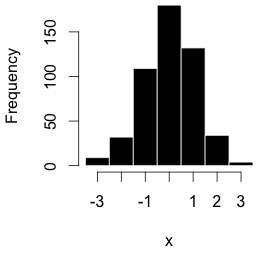
\includegraphics[width=0.4\textwidth]{histogram.png}
	\caption{Example of a histogram, $\Delta = 1$ (\href{https://en.wikipedia.org/wiki/Histogram}{src}).}
\end{figure}

\subsection{Parametric Probability Density Estimation}
In the other hands, one could find the \ac{prob} from $\displaystyle p = \int_{\mathcal{R}}p(y)dy \approx p(x)V$ where the region $\mathcal{R}$ is sufficiently small.\\
$\displaystyle \Rightarrow p(x) \approx \frac{K}{N.V}$, where $K$ is the number of data points in the region, $V$ is the volume of the region.

\subsection{Kernel Methods}
The kernel methods fix $V$ and determine $K$. The volume $V$ is the space restricted within a parzen window $k(u)$ that satisfies $k(u) \geq 0$.
\begin{align}
	&\text{A hyper-space cube:} && k(u) = \begin{cases}
		1\;\; if \;\; |u_i| \leq \frac{1}{2}h, \;\; i = 1, 2, \dots, D \\
		0\;\; else
	\end{cases} \\
	&\text{The number of points inside:} &&K = \sum_{n=1}^{N} k(x-x_n) \\
	&\text{The region \textit{volume}:} &&V = \int k(u) du = h^D\\
	&\text{The probability:} && \Rightarrow p(x) \approx \frac{K}{N.V} = \frac{1}{N.h^D}\sum_{n=1}^{N}k(x-x_n)
\end{align}
The \hlb{symmetric Gaussian kernel is a better substitution} for the asymmetric parzen window.
\begin{align}
	&\text{A Gaussian kernel:} && k(u) = \frac{1}{\sqrt{2\pi h^2}}\:exp\left(\frac{-u^2}{2h^2}\right) \\
	&\text{The region \textit{volume}:} &&V = \int k(u) du = 1 \\
	&\text{The probability:} && \Rightarrow p(x) \approx \frac{1}{N} \sum_{n=1}^{N} \frac{1}{(2\pi)^{D/2}h}\:exp\left(\frac{-||x-x_n||^2}{2h^2}\right)
\end{align}
For Kernel methods, $h$ is the \hlb{smoothing factor}.

Generalization: $k(u) \geq 0$, $\displaystyle \int k(u)du = 1$.

\hlr{Size of the hypersphere is proportional to $h^2$.}

\subsection{K-Nearest Neighbor}
When you fix $K$ and determine $V$, it leads to K-Nearest Neighbor.

\todo{Add image}

\begin{equation}
	p(x) \approx \frac{K}{NV}
\end{equation}
Here, $K$ is the \hlb{smoothing factor}.

\hlr{\begin{itemize}
		\item Too much bias $\Rightarrow$ too smooth
		\item Too much variance $\Rightarrow$ \underline{NOT} smooth enough
	\end{itemize}
	$\Rightarrow$ combine parametric methods to a mixture model}

\hlr{Mixture distribution = multi parametric model}

\subsection{Mixture of Gaussians}
\ac{MoG}, as \hlr{Generative Model}, is defined from the \ac{prob} sum of elemental Gaussians: $\displaystyle p(x|\theta) = \sum_{j=1}^{M}p(x|\theta_j)p(j)$, where $p(x|\theta_j)$ is a \hlr{mixture component}, $p(j) = \pi_j$ is the \hlr{weight of the component}
\begin{align}
	p(x|\theta_j) &= \frac{1}{\sqrt{2\pi}\sigma_j}\:exp\left[\frac{-(x-\mu_j)^2}{2\sigma_j^2}\right],\;\;p(j)=\pi_j, \;\;\sum\pi_j=1 \\
	p(x|\theta_j) &= \frac{1}{(2\pi)^{\frac{D}{2}}|\Sigma_j|^{\frac{1}{2}}}\:exp\left[-\frac{1}{2}(x-\mu_j)^T\Sigma_j^{-1}(x-\mu_j)\right]
\end{align}

\subsection{K-Means Clustering}
There are 3 steps:
\begin{itemize}
	\item Pick $K$ centroids
	\item Assign sample to the centroid
	\item Adjust centroids
\end{itemize}

Step 2 and 3 are repeated until there is no change.

This leads to a local optimum, depends on initialization. It's sensitive to \hlb{outliers}, detects \hlb{spherical clusters only}.

\todo{Add images}

Application: \eg, image compression.

\subsection{EM Clustering}
It's short for Expectation-Maximization. Assuming $N$ data points and $K$ Gaussians.
\begin{itemize}
	\item \textbf{E-Step:} Fix the Gaussians, find $\gamma_j(x)$, which represent the \hlr{responsibility of component $j$ for $x$}.
	\begin{equation}
		\gamma_j(x_n) = \frac{\pi_j \mathcal{N}\left(x_n|\mu_j,\Sigma_j\right)}
		{\sum_{k=1}^{K}\pi_k \mathcal{N}\left(x_n|\mu_k,\Sigma_k\right)} \;\;\forall j=1, 2, \dots, K, \;\; n=1, 2, \dots, N
	\end{equation}	
	\item \textbf{M-Step:} Fix $\gamma_j(x)$, update the Gaussians.
	\begin{align}
		\hat{N}_j &= \sum_{n=1}^{N}\gamma_j(x_n) \\
		\hat{\mu}_j &= \frac{1}{\hat{N}_j} \sum_{n=1}^{N} \gamma_j(x_n)x_n \\
		\hat{\pi}_j &= \frac{\hat{N}_j}{N} \\
		\hat{\Sigma}_j &= \frac{1}{\hat{N}_j} \sum_{n=1}^{N} \gamma_j(x_n) \left(x_n - \hat{\mu}_j\right)\left(x_n - \hat{\mu}_j\right)^T
	\end{align}
\end{itemize}
\hlb{Notes}:
\begin{itemize}
	\item Regularization with $\Sigma + \sigma_{min}I$
	\item Initialization $\mu_j$ with K-Means
	\item Hard-assignment: each data point to 1 class $\Rightarrow$ K-Means
	\item Soft-assignment: each data point $\Rightarrow$ \ac{prob} to fall into many classes $\Rightarrow$ EM Clustering
\end{itemize}

EM \hlr{needs more iteration}, because there are \hlr{more \ac{param}}.
% !TeX spellcheck = en_US
\chapter{Basic ML Problems}

\section{Linear Regression}
This is the simplest regression problem in \ac{ML}.

\hlb{Problem statement:} Given data points $\textbf{x}_i \in \mathbb{R}^D$ and their labels $y_i \in \mathbb{R}$, find the \textit{line} that fits these data points. The line is represented via parameters $\textbf{w} = [w_0, w_1, \dots, w_n]^T$. For each data point $\textbf{x}$ and its label $y$.

\hlb{Approach:}
\begin{align*}
	\bar{\textbf{x}} &= [1, x_0, \dots, x_n] && \text{(x bar - extended variable)}\\
	y \approx \hat{y} &= \bar{\textbf{x}} . \textbf{w} && \text{(y hat - predicted label)}\\
	\Rightarrow \frac{1}{2}e^2 &= \frac{1}{2} \left(y - \bar{\textbf{x}}.\textbf{w}\right)^2 && \text{(the squared error between true and predicted labels)}
\end{align*}
\begin{align}
	\mathcal{L}(\textbf{w}) &= \frac{1}{2} \sum_{i=1}^{N} \left(y_i - \bar{\textbf{x}}_i.\textbf{w}\right) ^2 && \text{(the loss function for all points)} \\
	\mathcal{L}(\textbf{w}) &= \frac{1}{2N} \sum_{i=1}^{N} \left(y_i - \bar{\textbf{x}}_i.\textbf{w}\right) ^2 && \text{(the average loss)} \\
	\textbf{w}^* &= \underset{\textbf{w}}{\text{argmin}}\,\mathcal{L}(\textbf{w}) && \text{(the weights that minimize the loss function)} \\
	\mathcal{L}(\textbf{w}) &= \frac{1}{2} ||\textbf{y}-\overline{\textbf{X}}.\textbf{w}||^2_2 && \text{(using matrix form)}
\end{align}

with $\overline{\textbf{X}} = \begin{bmatrix}
	\bar{\textbf{x}}_1 \\
	\bar{\textbf{x}}_2 \\
	\vdots \\
	\bar{\textbf{x}}_n
\end{bmatrix}$
and $\textbf{y} = \begin{bmatrix}
	y_1 \\
	y_2 \\
	\vdots \\
	y_n	
\end{bmatrix}$

\hlb{Solution:}
\begin{align}
	&\frac{\partial\mathcal{L}(\textbf{w}^*)}{\partial\textbf{w}} = \overline{\textbf{X}}^T \left( \overline{\textbf{X}} \textbf{w}^* - \textbf{y} \right) = 0 \\
	\Leftrightarrow \; &\overline{\textbf{X}}^T\overline{\textbf{X}}\textbf{w}^* = \overline{\textbf{X}}^T \textbf{y} \\
	\Leftrightarrow \; &\textbf{w}^* = \left( \overline{\textbf{X}}^T \overline{\textbf{X}} \right)^\dagger \overline{\textbf{X}}^T \textbf{y}
\end{align}
in which, $A^\dagger$ (A dagger) is the pseudo inverse of a matrix, because $A$ might not be inverse-able. {\color{red} \boxed{A^\dagger = \left(A^TA\right)^{-1}A^T}}\\

\note
\begin{itemize}
	\item Sensitive to outliers $\Rightarrow$ pre-processing
	\item Multi-variable:
	\begin{align*}
		\mathcal{L}(\textbf{w}) &= \frac{1}{2N} ||\textbf{y}-\overline{\textbf{X}}.\textbf{w}||^2_2 \\
		\Rightarrow\; \nabla_\textbf{w}\mathcal{L}(\textbf{w}) &= \frac{1}{N} \overline{\textbf{X}}^T (\overline{\textbf{X}}\textbf{w}-\textbf{y})
	\end{align*}
\end{itemize}
\section{Linear Discriminant Functions}
\label{sec:linear-classification}
\hlb{Problem statement:} of general classification problem
\begin{itemize}
	\item Given: training set $\textbf{X} = \{\textbf{x}_1, \textbf{x}_2, \dots, \textbf{x}_N\}$ with target values (labels) $\textbf{T} = \{\textbf{t}_1, \textbf{t}_2, \dots, \textbf{t}_N\}$.
	\item Goal: take a new input $\textbf{x}$ and assign it to one of $K$ classes $C_k$\\
	$\Rightarrow$ Learn a discriminant function $y(x)$ to perform the classification
\end{itemize}
\hlb{Approach:}
\begin{itemize}
	\item 2-class problem: Binary target values: $t_n \in \{0, 1\}$\\
	\Eg of discriminant function: $y(x) > 0 \Rightarrow$ class $C_1$, else $C_2$
	\item K-class problem: 1-of-K coding scheme, \eg: $\textbf{t}_n = [0, 1, 0, 0, 0]^T$
	\item Extension to multiple classes: one-vs-all, one-vs-one classifiers
\end{itemize}
\subsection{Least-Squares Classification}
With above problem statement, consider $K$ classes described by linear models:
\begin{align*}
	y_k(\textbf{x}) &= \textbf{w}^T_k\textbf{x} + w_{k0} && k=1, \dots, K \\
	\Rightarrow \textbf{y}(\textbf{x}) &= \widetilde{\textbf{W}}^T\widetilde{\textbf{x}} && \text{(using vector notation)} \\
	\textbf{Y}(\widetilde{\textbf{X}}) &= \widetilde{\textbf{X}}\widetilde{\textbf{W}} && \text{(for the entire dataset)}
\end{align*}
In which output $\textbf{y}$ in 1-of-K notation, and can be compared to the target value
\[\textbf{t}=[t_1, \dots, t_k]^T\]
\hlb{Solution:} minimize the sum-of-squares error $E(\textbf{w})$
\begin{align*}
	E(\textbf{w}) &= \frac{1}{2} \sum_{n=1}^{N} \left(\textbf{y} - \textbf{t}\right)^2 = 
	\frac{1}{2} \sum_{n=1}^{N} \sum_{k=1}^{K} \left(\textbf{w}_k^T\textbf{x}_n-t_{kn}\right)^2 \\
	\Rightarrow \widetilde{\textbf{W}}^* &=  \left( \widetilde{\textbf{X}}^T \widetilde{\textbf{X}} \right)^{-1} \widetilde{\textbf{X}}^T T = \widetilde{\textbf{X}}^\dagger T
\end{align*}
\note Least-squares is very sensitive to outliers!\\
The error function penalizes predictions that are “too correct”.

\subsection{Generalized Linear Discriminant}
\begin{equation}
	y_k(x) = \sum_{j=1}^{M}w_{kj}\phi_j(x) + w_{k0} = \sum_{j=0}^M w_{kj}\phi_j(x), \tab \phi_0(x) = 1
\end{equation}

\subsection{Generalized Linear Models}
\begin{itemize}
	\item Linear Model:
	\begin{equation}
		y(\textbf{x}) = \textbf{w}^T\textbf{x} + w_0
	\end{equation}	
	\item Generalized Linear Model:
	\begin{equation}
		y(\textbf{x}) = g(\textbf{w}^T\textbf{x} + w_0)
		\label{eq:generalized-linear-model}
	\end{equation}	
	In which $g(\cdot)$ is called an \hlb{activation function} and may be nonlinear
\end{itemize}

\section{Logistics Regression}

Though named as "regression", logistics regression is used for classification problem, just like Linear Discriminant (\secref{sec:linear-classification}).

\hlb{Problem:} In many of binary classification problems (classification problem with 2 classes), it's rather hard (or even impossible) to be certain about the class of the output, and the training data is not linear separable. Instead of a hard threshold, we could have a soft one, represent by the \ac{prob} belonging to either classes.
\begin{figure}[hbt!]
	\centering
	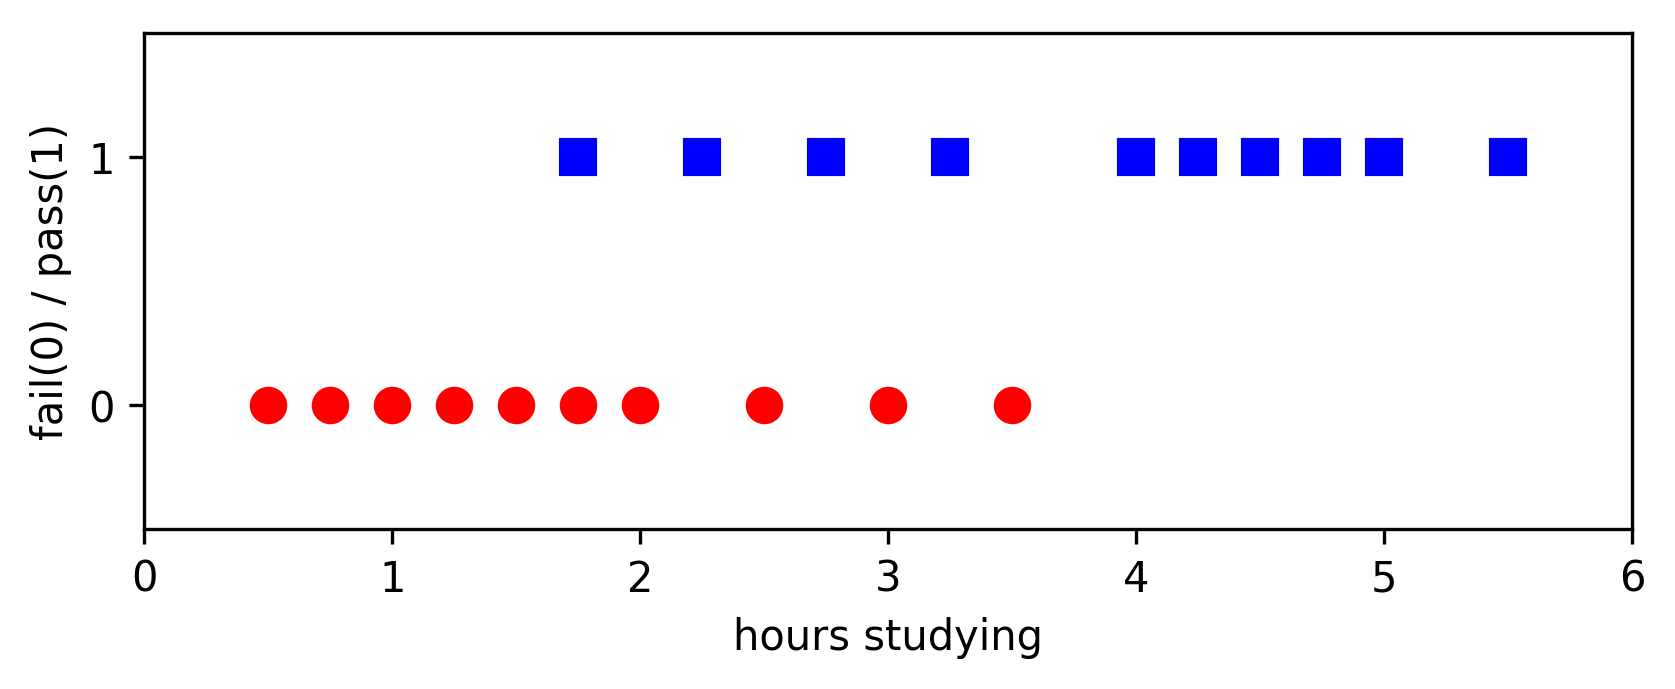
\includegraphics[width=0.79\textwidth]{sigmoid-example.png}
	\caption{Example of exam results based on study hours (\href{https://machinelearningcoban.com/2017/01/27/logisticregression/}{src}). Given the number of hours, instead of predicting whether fail or pass, the model predicts the \ac{prob} that the student will pass, or fail.}
\end{figure}

The sigmoid function gives a nice nonlinear transition for the \ac{prob}. The further the data point is from the threshold, the higher the \ac{prob} it belongs to one class, and small to the others.
\begin{align}
	f(s) 		&= \frac{1}{1 + e^{-s}} \overset{\triangle}{=} \sigma(s) \\
	s 			&= \text{ln} \left( \frac{\sigma}{1-\sigma} \right) \\
	\sigma'(s)	&= \sigma(s) \left( 1- \sigma(s) \right)
\end{align}
Thus, if we use the sigmoid function as the activation function for \eqref{eq:generalized-linear-model}:
\begin{align}
	s &= \textbf{w}^T \textbf{x} \\
	y &= \sigma(s)\\
	\Rightarrow \; \frac{\partial y}{\partial \textbf{w}}&= \frac{\partial y}{\partial s} \frac{\partial s}{\partial \textbf{w}} = y(1-y) \textbf{x}
	\label{eq:sigmoid}
\end{align}
\begin{figure}[hbt!]
	\centering
	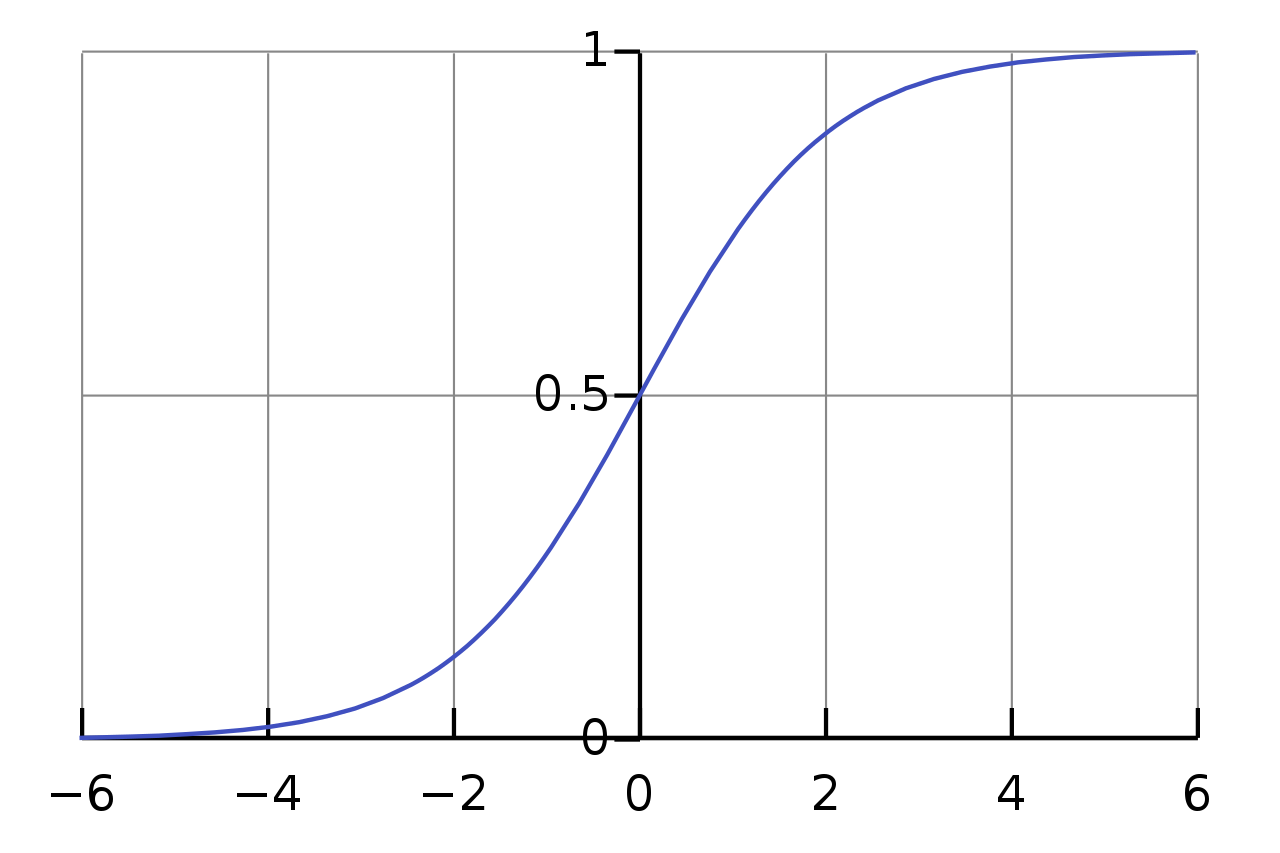
\includegraphics[width=0.5\textwidth]{sigmoid.png}
	\caption{Sigmoid function (\href{https://en.wikipedia.org/wiki/Sigmoid_function}{src}).}
\end{figure}

\hlb{Approach:}
\begin{itemize}
	\item Design of the error function.\\
	Assume that the \ac{prob} of data point $\textbf{x}$ falls into class 1 is $f(\textbf{w}^T\textbf{x})$ and class 0 is $1-f(\textbf{w}^T\textbf{x})$. With $z_i = f(\textbf{w}^T\textbf{x}_i)$:
	\begin{equation}
		\begin{cases}
			P(y_i=1|\textbf{x}_i; \textbf{w}) &= f(\textbf{w}^T\textbf{x}_i) = z_i \\
			P(y_i=0|\textbf{x}_i; \textbf{w}) &= 1 - f(\textbf{w}^T\textbf{x}_i) =1 - z_i
		\end{cases} \Leftrightarrow P(y_i | \textbf{x}_i; \textbf{w}) = z_i^{y_i}(1-z_i)^{1-y_i}
	\end{equation}
	With the aim to find the model \ac{param} that maximizes the data \ac{prob} (\subsecref{subsec:mle}):
	\begin{align*}
		& \textbf{w}^* = \arg \underset{\textbf{w}}{\max}\;P(\textbf{y}|\textbf{X; w}) && \\
		\iff & \textbf{w}^* = - \arg \underset{\textbf{w}}{\min} \log P(\textbf{y}|\textbf{X; w}) && \text{(negative log-likelihood)} \\
		& P(\mathbf{y}|\mathbf{X}; \mathbf{w}) = \prod_{i=1}^N P(y_i| \mathbf{x}_i; \mathbf{w}) = \prod_{i=1}^N z_i^{y_i}(1 - z_i)^{1- y_i} && \text{(independence assumption)} \\
		\Rightarrow & - \log P(\textbf{y}|\textbf{X; w}) = - \sum_{i=1}^{N} [ y_i\log z_i + (1-y_1)\log (1-z_i) ] && \text{(the cross entropy error)}
	\end{align*}
	
	\item Optimization with \ac{SGD}:
	\begin{align}
		& \textbf{w} = \textbf{w} - \eta.\frac{\partial J}{\partial \textbf{w}}, \quad \text{($\eta$ as the learning rate)}
		\label{eq:log-reg-sgd}\\			
		& J(\textbf{w}, \textbf{x}_i, y) = -\left( y_i\log z_i + (1-y_i)\log(1-z_i) \right), \quad \text{data point $(\textbf{x}_i, y_i)$} \\
		\Rightarrow \; &\frac{\partial J}{\partial \textbf{w}} = - \left( \frac{y_i}{z_i} - \frac{1-y_i}{1-z_i} \right) \frac{\partial z_i}{\partial\textbf{w}} = \frac{z_i - y_i}{z_i(1-z_i)} \frac{\partial z_i}{\partial\textbf{w}} \\
		& \frac{\partial z_i}{\partial \textbf{w}} = z_i(1-z_i) \textbf{x}_i \tab \text{(the beauty of sigmoid function, \eqref{eq:sigmoid})} \\
		\Rightarrow \; &\frac{\partial J}{\partial \textbf{w}} = (z_i - y_i) \textbf{x}_i\\
		\Rightarrow \; &w = w + \eta (y_i - z_i) \textbf{x}_i \tab \text{(replace into \eqref{eq:log-reg-sgd})}
	\end{align}
\end{itemize}

\note Require less \ac{param}, only $D$ with $D$ as the \ac{no} dimensions, compared to Gaussians with $\displaystyle \left[\frac{M(M+5)}{2}+1\right]$ \ac{param}.

\section{Softmax Regression}

Softmax Regression is the generalization of Logistics Regression for multiple-class classification problem. Thus, it is also known as: \hlr{Multinomial Logistics Regression, Maximum Entropy Classifier}. Logistics Regression can only be applied for binary classification problem. Given $C$ classes, we would need multiple one-vs-all or one-vs-one classifiers. Softmax regression offers a better alternative.
\begin{align}
	&z_i = \textbf{w}^T \textbf{x}_i\\
	&a_i = \frac{\text{exp}(z_i)}{\sum_{j=1}^{C}\text{exp}(z_j)}\\
	&\begin{cases}
		a_i > 0, \tab a_i \text{ represents the \ac{prob} the input belongs to class }C_i\\
		\sum a_i = 1 \\
		z_m > z_n \iff a_m > a_n \quad \text{(order)}
	\end{cases}
\end{align}

There are cases that one output $z_i$ is significantly greater than the others, which will lead to numerical error while coding. In these cases, the following Softmax version is more stable:
\begin{equation}
	a_i = \frac{\text{exp}(z_i)}{\sum_{j=1}^{C}\text{exp}(z_j)} = \frac{\text{exp}(z_i - c)}{\sum_{j=1}^{C}\text{exp}(z_j - c)},\quad c = \underset{i}{\max}\;z_i
\end{equation}

For the one hot coding representation, for each input $\textbf{x}$, the softmax regression model calculate a output vector $\textbf{a} = \textbf{W}^T \textbf{x}$. The loss function will be build to represent the difference between output $\textbf{a}$ and the real label $\textbf{y}$. Vector $\textbf{a}$ itself is a \ac{prob} distribution of the input belongs to different classes. Instead of choosing the squared error function, cross-entropy is a better alternative to represent the difference between two \ac{prob} distributions (\secref{sec:cross-entropy}). As mentioned before, $\textbf{q} >0$, thus, we can't choose $\textbf{q} = \textbf{y}$.
\begin{align}
	&J(\textbf{W},\textbf{x}_i,\textbf{y}_i) = - \sum_{i=1}^{N} \sum_{j=1}^{C} y_{ij}\,\text{log}(a_{ij}) && \text{for each data point } (\textbf{x}_i, \textbf{y}_i) \\
	&\frac{\partial J_i(\textbf{W})}{\partial \textbf{W}} = \textbf{x}_i \textbf{e}_i^T = \textbf{x}_i (\textbf{a}_{i} - \textbf{y}_{i})^T && \text{(the gradient)}\\
	&\textbf{W} = \textbf{W} + \eta \textbf{x}_i (\textbf{y}_i - \textbf{a}_i)^T && \text{(\ac{SGD}, \href{https://machinelearningcoban.com/2017/02/17/softmax/}{machinelearningcoban.com})}
\end{align}

\section{SVM}

\ac{SVM}

\subsection{Hard Margin \ac{SVM}}

\hlb{Problem:} Give $N$ data points $\textbf{x}_i$ and their labels $y_i \in \{-1, 1\}$, find the line that separate these points into two classes while maximize the margin.

\begin{figure}[hbt!]
	\centering
	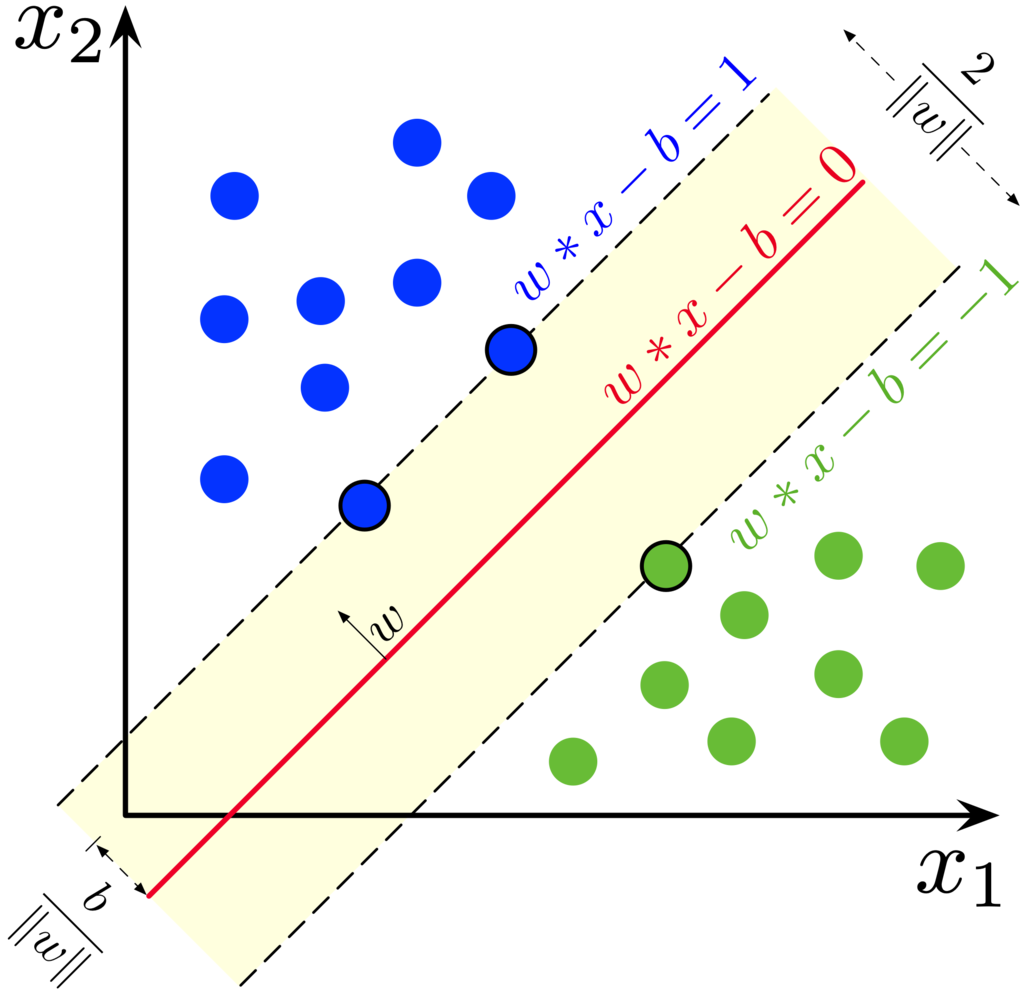
\includegraphics[width=0.5\textwidth]{svm.png}
	\caption{Example of \ac{SVM} (\href{https://en.wikipedia.org/wiki/Support-vector_machine}{src}).}
\end{figure}

\begin{align}
	&margin = \underset{n}{\min} \frac{y_n (\textbf{w}^T \textbf{x}_n) +b}{||\textbf{w}||_2}\\
	\Rightarrow\; &(\textbf{w},b) = \underset{\textbf{w}, b}{\arg\max} \left\{ \underset{n}{\min} \frac{y_n (\textbf{w}^T \textbf{x}_n) +b}{||\textbf{w}||_2} \right\} \\
	\Rightarrow\; &(\textbf{w},b) = \underset{\textbf{w}, b}{\arg\max} \left\{ \frac{1}{||\textbf{w}||_2} \underset{n}{\min}\left[ y_n(\textbf{w}^T \textbf{x}_n+b) \right] \right\}
\end{align}

For simplicity, we can assume that: $\underset{n}{\min}\left[ y_n(\textbf{w}^T \textbf{x}_n+b) \right] = 1$. Thus, the original problem can be transform to:

\hlb{Problem:} Find $\displaystyle (\textbf{w},b) = \underset{\textbf{w}, b}{\arg\min} \frac{1}{2}||\textbf{w}||^2_2$ that subject to:
\begin{equation*}
	1-y_n(\textbf{w}^T\textbf{x}_n+b) \leq 0, \quad \forall n = 1, 2, \dots, N
\end{equation*}
This is a well-studied optimization problem, solved with Lagrange's method.

\hlb{Approach:} The Lagrange's method

\hlr{The primal formulation of \ac{SVM}:}
\begin{align}
	& \mathcal{L}(\textbf{w}, b, \boldsymbol{\lambda}) = \frac{1}{2} ||\textbf{w}||^2_2 + \sum_{n=1}^{N} \lambda_n [1 - y_n(\textbf{w}^T\textbf{x}_n+b)], \quad \lambda_n \geq 0 \quad \forall n\\
	& \frac{\partial \mathcal{L}(\textbf{w}, b, \boldsymbol{\lambda})}{\partial\textbf{w}} = 0 \Rightarrow \textbf{w} = \sum_{n=1}^{N} \lambda_n y_n \textbf{x}_n \\
	& \frac{\partial \mathcal{L}(\textbf{w}, b, \boldsymbol{\lambda})}{\partial\textbf{b}} = 0 \Rightarrow \sum_{n=1}^{N} \lambda_n y_n =0
\end{align}
\hlr{The dual formulation of \ac{SVM}:}
\begin{align}
	\Rightarrow & g(\boldsymbol{\lambda}) = \sum_{n=1}^{N} \lambda_n - \frac{1}{2} \sum_{n=1}^{N} \sum_{m=1}^{N} \lambda_n \lambda_m y_n y_m \textbf{x}_n^T \textbf{x}_m \\
	\text{Set } & \textbf{V} = \left[ y_1\textbf{x}_1, y_2\textbf{x}_2, \dots, y_N\textbf{x}_N \right] \\
	\Rightarrow & g(\boldsymbol{\lambda}) = - \frac{1}{2} \boldsymbol{\lambda}^T \textbf{V}^T \textbf{V} \boldsymbol{\lambda} + 1^T\boldsymbol{\lambda} \qquad \text{is \hlb{concave} with} \quad \lambda_i \geq 0, \quad \sum_{n=1}^{N} \lambda_n y_n = 0
\end{align}
\hlr{$\Rightarrow$ Find $\lambda$ by solving Quadratic Programming}\\
Then use \ac{KKT} conditions to find $\textbf{w}, b$:\\
\hlre{S = \{n \;|\; \lambda_n \neq0\} \Rightarrow \begin{cases}
	b = \frac{1}{N_S} \sum_{n\in S} \left( y_n - \sum_{m \in S} \lambda_m y_m \textbf{x}_m^T \textbf{x}_n \right)\\
	\textbf{w} = \sum_{m \in S} \lambda_m y_m \textbf{x}_m
\end{cases}}

\subsection{Soft Margin \ac{SVM}}
\begin{itemize}
	\item Hard margin \ac{SVM}:
	\begin{align*}
		&(\textbf{w},b) = \underset{\textbf{w}, b}{\arg\min} \frac{1}{2}||\textbf{w}||^2_2 \\
		\text{subject to}\quad &y_n(\textbf{w}^T\textbf{x}_n+b) \geq 1 \quad \forall n
	\end{align*}
	\item Soft margin \ac{SVM}:
	\begin{align*}
		&(\textbf{w},b, \xi) = \underset{\textbf{w}, b, \xi}{\arg\min} \frac{1}{2} || \textbf{w} ||^2_2 + C \sum_{n=1}^{N} \xi_n \\
		\text{subject to}\quad &\begin{cases}
			y_n(\textbf{w}^T\textbf{x}_n+b) \geq 1 -\xi_n\\
			\xi_n \geq 0
		\end{cases} \quad \forall n 
	\end{align*}
\end{itemize}
\hlr{$C$ and the margins are in-proportional: $\begin{cases}
		C\uparrow \quad\Rightarrow\quad margin \downarrow \\
		C\downarrow \quad\Rightarrow\quad margin \uparrow
\end{cases}$}

The \textit{"Soft"} constraints:
\begin{equation*}
	y_n(\textbf{w}^T\textbf{x}_n+b) \geq 1 -\xi_n \quad \iff \quad 1 - \xi_n -y_n(\textbf{w}^T \textbf{x}_n +b) \leq 0 \quad \forall n
\end{equation*}

\hlb{Problem:} Find $\displaystyle (\textbf{w},b, \xi) = \underset{\textbf{w}, b, \xi}{\arg\min} \frac{1}{2} || \textbf{w} ||^2_2 + C \sum_{n=1}^{N} \xi_n$ that subject to:
\begin{equation*}
	\begin{cases}
		1 - \xi_n -y_n(\textbf{w}^T \textbf{x}_n +b) \leq 0 \\
		- \xi_n \leq 0
	\end{cases} \quad \forall n
\end{equation*}

\hlb{Approach:} Lagrange's method with $\lambda_i \geq 0$ and $\mu_i \geq 0$:
\begin{align}
	&\mathcal{L}(\textbf{w}, b, \boldsymbol{\xi, \lambda, \mu}) = \frac{1}{2} || \textbf{w} ||^2_2 + C \sum_{n=1}^{N} \xi_n + \sum_{n=1}^{N} \lambda_n [ 1-\xi_n - y_n(\textbf{w}^T \textbf{x}_n +b) ] - \sum_{n=1}^{N} \mu_n\xi_n \\
	&\frac{\partial \mathcal{L}}{\partial \textbf{w}} = 0 \iff \textbf{w} = \sum_{n=1}^N \lambda_n y_n \textbf{x}_n\\
	&\frac{\partial \mathcal{L}}{\partial b} = 0 \iff \sum_{n=1}^N \lambda_n y_n = 0\\
	&\frac{\partial \mathcal{L}}{\partial \xi_n} = 0 \iff \lambda_n = C - \mu_n\\
	&g(\boldsymbol{\lambda, \mu}) = \underset{\textbf{w}, b, \boldsymbol{\xi}}{\inf} \mathcal{L}(\textbf{w}, b, \boldsymbol{\xi, \lambda, \mu})\\
	\Rightarrow &g(\boldsymbol{\lambda, \mu}) = \sum_{n=1}^{N} \lambda_n - \frac{1}{2} \sum_{n=1}^{N} \sum_{m=1}^{N} \lambda_n \lambda_m y_n y_m \textbf{x}_n^T \textbf{x}_m = g(\boldsymbol{\lambda})\\
	\Rightarrow &\boldsymbol{\lambda} = \underset{\boldsymbol{\lambda}}{\arg\max} g(\boldsymbol{\lambda}) \quad \text{subject to} \quad \begin{cases}
		\sum_{n=1}^{N} \lambda_n y_n=0\\
		0 \leq \lambda_n \leq C \quad \forall n
	\end{cases}
\end{align}
After finding $\boldsymbol{\lambda}$:
\begin{align}
	&\mathcal{M} = \{ n \;|\; 0 < \lambda_n < C \} &&\Rightarrow b=\frac{1}{N_M} \sum_{n \in \mathcal{M}} \left( y_n - \sum_{m \in \mathcal{S}} \lambda_m y_m \textbf{x}_m^T \textbf{x}_n \right)\\
	&\mathcal{S} = \{ m \;|\; 0 < \lambda_m \leq C \} &&\Rightarrow \textbf{w} = \sum_{m \in \mathcal{S}} \lambda_m y_m \textbf{x}_m
\end{align}
\begin{itemize}
	\item $\begin{cases}
		\lambda_n =0\\
		\xi_n =0
	\end{cases} \Rightarrow$ \hlr{Safe points} 
	\item $\begin{cases}
		0 < \lambda_n < C\\
		\xi_n =0
	\end{cases} \Rightarrow$ \hlr{Marginal points} 
	\item $\lambda_n =C \quad \begin{cases}
		\xi_n  \leq 1 \quad\Rightarrow \text{\hlr{still correct}}\\
		\xi_n > 1 \quad\Rightarrow \text{\hlr{incorrect}}
	\end{cases}$
\end{itemize}

\subsection{Kernel Support Vector Machine}
\hlb{Mercer's Conditions:} kernel \ac{func} must theoretically satisfy.\\
In practice, however, some acceptable kernels don't satisfy the Mercer's conditions.
\begin{equation}
	\sum_{n=1}^N\sum_{m=1}^N k(x_n, x_m) c_n c_m \geq 0 \quad \forall c_i \in \mathbb{R}, i =1, 2, \dots, N
\end{equation}
\Eg kernel functions:
\begin{align*}
	&k(x,z) = x^T z && \hlr{linear}\\
	&k(x,z) = (\gamma x^T z + r)^d && \hlr{polynomial}\\
	&k(x,z) = \exp(-\gamma ||x-z||^2_2), \quad \gamma>0 && \hlr{\ac{RBF}}\\
	&k(x,z) = \tanh(\gamma x^T z + r) && \hlr{sigmoid}
\end{align*}

\chapter{Ensembles}
Ensemble of Models are also known as addictive models.

\section{Error Reduction}

\todo{Explanation}

\Eg: bagging
\begin{align}
	&y_{COM}(x) = \frac{1}{M} \sum_{m=1}^{M} y_m(x)\\
	&y(x) = h(x) + \varepsilon(x)\\
	&\mathbb{E}_x = \left[ y_m(x) - h(x) \right]^2 = \mathbb{E}_x \left[ \varepsilon_m(x)^2 \right]\\
	\Rightarrow &\mathbb{E}_{AV} = \frac{1}{M} \sum_{m=1}^{M} \mathbb{E}_x \left[ \varepsilon_m (x)^2 \right]\\
	&\mathbb{E}_{COM} = \mathbb{E}_x \left[ \left\{ \frac{1}{M} \sum_{m=1}^{M} y_m(x) - h(x) \right\}^2 \right] = \mathbb{E}_x \left[ \left\{ \frac{1}{M} \sum_{m=1}^{M} \varepsilon_m(x) \right\}^2 \right]
\end{align}

$\Rightarrow$ if $\begin{cases}
	\text{errors have 0 mean:} \qquad\qquad \mathbb{E}_x[\varepsilon_m(x)]=0\\
	\text{errors are uncorrelated:} \qquad \mathbb{E}_x[\varepsilon_m(x) \varepsilon_j(x)]=0 \text{ (unrealistic??)}
\end{cases} \Rightarrow \mathbb{E}_{COM} = \frac{1}{M} \mathbb{E}_{AV}$

However, in general, $\mathbb{E}_{COM} < \mathbb{E}_{AV}$

\note The weak classifiers have to be unstable algorithms, \ie, decision trees, neural network; \hlr{NOT} nearest neighbor, \ac{SVM}, linear regression.

\section{Bagging}
\label{sec:bagging}
\begin{itemize}
	\item Check \href{https://youtu.be/2Mg8QD0F1dQ}{Udacity's video}
	\item \ac{aka} Bootstrap aggregating
	\item Average $\approx$ 63\%
\end{itemize}

\todo{Image}
\begin{itemize}
	\item Split the given data set into train and test set
	\item Assume train set with $n$ data points
	\item Pick $n'$ data points into each bag $D_i$,\quad $\frac{n'}{n} < 1 (\approx 60\%)$
	\item Create $m$ data bags: $D_1, D_2, \dots, D_m$
	\item Learn a model $M_i$ from each bag $D_i$
	\item The final output is the average of models' outputs:
	\[y = \frac{1}{m} \sum_{i=1}^{m} f(M_i)\]
	\item \hlr{Random with replacement:} bag $i$ can have multiple times data point $\textbf{x}_i$
	\item \hlr{Simple, easy to implement, commonly used}
\end{itemize}
\note Practically, resampling with replacement is \hlb{usually unnecessary}, since \ac{SGD} and random initialization usually makes the models sufficiently independent.

\section{Boosting}
\begin{itemize}
	\item Adaboost
	\item Gradient boosting
	\item Xgboost (extreme gradient boosting)
	\item Gentle Boost (cross entropy error)
\end{itemize}

\subsection{Adaboost}
Resources:
\begin{itemize}
	\item \href{https://youtu.be/LsK-xG1cLYA}{AdaBoost, Clearly Explained}
	\item 
\end{itemize}

\begin{enumerate}
	\item First weak classifier
	\item Calculate error $J \Rightarrow \varepsilon$\\
	in case of normalization $w \Rightarrow \sum w = 1 \Rightarrow \varepsilon = J$
	\item Calculate amount of say $\alpha$ from $\varepsilon$
	\item Update $w$ with $\alpha$ (normalize $w$)
	\item 2nd weak classifier with new weight $w$ or sample on new $w$
\end{enumerate}

\begin{itemize}
	\item Ensembles of Classifiers: $K$ independent classifiers, error \ac{prob} < 0.5
	\item Suitable for unstable algorithms (\ie, decision trees, neural networks)
	\item Not good with stable methods (\ie, nearest neighbors, \ac{SVM}s, linear regression)
\end{itemize}

\todo{EXPLANATION?}
\begin{align}
	& -g(x_i) = -\frac{\partial \mathcal{L} (y_i, F(x_i))}{\partial F(x_i)} \\
	\Rightarrow & \text{Regression model: } \quad h_i \text{ for } (x_i, -g(x_i))\\
	\Rightarrow & F:= F + \rho h, \quad \rho = 1
\end{align}

\todo{EXPLANATION?}\\
\hlb{Problem:} \begin{itemize}
	\item Given: $N$ data points and their labels $(x_n, t_n)$
	\item Goal: find $M$ weak classifiers $h_m(x)$
\end{itemize}
\begin{align}
	w_n^{(0)} &= \frac{1}{N} && \text{initial data weights}\\
	J_m &= \sum_{n=1}^{N} w_n^{(m)} I\left( h_m(x) \neq t_n \right) && \text{weighted error function}\\
	\varepsilon_m &= \frac{\sum_{n=1}^{N} w_n^{(m)} I\left( h_m(x) \neq t_n \right) }{\sum_{n=1}^{N} w_n^{(m)}} && \text{(normalized) weighted error}\\
	\alpha_m &= \ln \left(\frac{1-\varepsilon_m}{\varepsilon_m}\right) && \text{classifier weights}\\
	w_n^{(m+1)} &= w_n^{(m)}.\exp\left\{ \alpha_m I\left( h_m(x) \neq t_n \right)\right\} && \text{updated data weights}\\
	H(x) &= sign\left( \sum_{m=1}^{M} \alpha_m h_m(x) \right) && \text{final classification}
\end{align}

\todo{EXPLANATION?}
\hlr{Adaboost}
\begin{align}
	&F(x) = sign \left( \sum_{m=1}^{M} \theta_m f_m(x) \right)\\
	&w(x_i, y_i) = \frac{1}{n} \qquad\qquad \text{initial weights for each data}\\
	&\varepsilon_m = \mathbb{E}_{\varepsilon_m} \left[ 1_{y \neq f(x)} \right]\\
	\Rightarrow\; &\theta_m = \frac{1}{2} \ln\left( \frac{1-\varepsilon_m}{\varepsilon_m} \right) \qquad\qquad \text{Update rule}\\
	&w_{m+1}(x_i, y_i) = \frac{w_m(x_i, y_i) \exp[-\theta_m y_i f_m(x_i)]}{z_m} \qquad\qquad \text{update weights}\\
	&(z_m \text{ is the normalization factor})
\end{align}

\todo{Explanation:}
\hlr{Exponential error used in Adaboost}
\begin{itemize}
	\item Fast convergence
	\item No penalty for too correct
	\item Less robust to outlier
\end{itemize}
\todo{Add function graph}

\subsection{Gradient Boosting (Regression)}
Check: A Gentle Introduction to Gradient Boosting - Cheng Li, CCS, Northeastern Uni
\begin{align}
	& (x_i, y_i) \text{ and first model } F_1(x)\\
	\Rightarrow & \text{ fit } F_2(x) \text{ to } (x_i, y_i - F_1(x_i)), \quad y_i - F_1(x_i)=h(x_i)	\text{ as the residuals}\\
	& J = \sum \mathcal{L} (y_i, F(x_i))\\
	\Rightarrow & F_{i+1} = F_i + h_i\\
	&{\color{red} \mathcal{L} = \frac{(y_i - F_i)^2}{2} \Rightarrow -g = y_i - F_i(x_i)} \\
	\label{eq:1}
	&{\color{red} \mathcal{L} = |y-F| \qquad \qquad \text{(absolute loss)} }\\
	\label{eq:2}
	&{\color{red} \mathcal{L} =\begin{cases}
			\frac{1}{2} (y-F)^2 \qquad\qquad \text{if } |y-F| \geq \delta\\
			\delta \left( |y-F| - \frac{\delta}{2} \right) \qquad \text{if } |y-F| <\delta
	\end{cases} \qquad \text{(Huber loss)}} 
\end{align}

The two loss functions \eqref{eq:1} and \eqref{eq:2} are less sensitive to outliers

\section{Information}

Mutual Information: \href{https://www.youtube.com/watch?v=d7AUaut6hso}{YouTube}, \href{https://www.youtube.com/watch?v=U9h1xkNELvY}{YouTube}.

\section{Decision Trees}

Iterative Dichotomiser 3: \href{https://machinelearningcoban.com/2018/01/14/id3/}{MLCoBan}
Detail Example calculation: \href{https://medium.com/@rishabhjain_22692/decision-trees-it-begins-here-93ff54ef134}{medium.com}, 
\href{https://clearpredictions.com/Home/DecisionTree}{blog}

CART: Gini Index: \href{http://www.learnbymarketing.com/481/decision-tree-flavors-gini-info-gain/}{blog}

Random forest: \href{https://www.youtube.com/watch?v=D_2LkhMJcfY}{YouTube}

\todo{Add image} root node, non-leaf node has 2 (or more) child node, leaf/terminal node. All non-leaf nodes have 2 child nodes $\Rightarrow$ binary decision tree

Iterative Dichotomiser 3 (ID3) only for categorical attribute (discrete)

Classification and Regression Tree (CART) for both categorical and continuous.

6 questions:
\begin{itemize}
	\item Bin / multi valued
	\item when node $\rightarrow$ leaf
	\item Deal impure nodes?
	\item how to select query
	\item pruned?
	\item missing attribute?
\end{itemize}

Impurity measures:
\begin{itemize}
	\item Misclassification: $i(s_j) = 1 - \underset{k}{\max}\;p(C_k | s_j)$
	\item Information gain: $C$ classes with $N_C$ as the number of members in each class
	\begin{equation}
		H(S) = - \sum_{c=1}^{C} \frac{N_C}{N} \log \left(\frac{N_C}{N}\right) \qquad \text{entropy at a node}
	\end{equation}
	Choose attribute $X$ $\Rightarrow$ $K$ child nodes: $S_1, S_2, \dots, S_k$ with $m_k$ elements
	\begin{align}
		&H(x, S) =  \sum_{k=1}^{K} \frac{m_k}{N} H(S_k) \qquad \text{entropy sum with weights} \\
		\Rightarrow\; &G(x, S) = H(S) - H(x, S) \qquad \text{information gain}\\
		&x^* = \underset{x}{\arg\max}\;G(x, S) = \underset{x}{\arg\min}\;H(x, S)
	\end{align}
	\hlr{Reduction in entropy = gain in information}
	\item Gini Index:
	\begin{align}
		i(s_j) &= \sum_{k \neq l} p(C_k | s_j) p(C_l, s_j) \qquad \text{variance impurity at node } s_j\\
		&= \frac{1}{2} \left[1- \sum_{k} p^2(C_k, s_j) \right]\\
		H(x, s_j) &= \sum_{k=1}^{K} \frac{m_k}{N} i(s_j)\\
		\Rightarrow x^* &= \min H(x, s_j)
	\end{align}
	\item Chi-square: $\displaystyle = \sqrt{\frac{(actual - expected)^2}{expected}}$, $\arg\max$\\
	CHAID: Chi-square Automatic Interaction Detector
	\item Reduction in Variance, $\arg\min$\\
	\begin{equation}
		i(s_j) = \frac{\sum (x-\bar{x})^2}{n}
	\end{equation}
\end{itemize}

\todo{Add image}

\hlr{Stopping and Pruning is more IMPORTANT}

\subsection{Stopping Conditions}
\begin{itemize}
	\item Prevent over-fitting = \hlr{Prepruning}
	\item $H(\mathcal{S}) = 0$: entropy $= 0 \Rightarrow \forall \text{ points } \in$ each class
	\item \ac{no} members in each node < a certain threshold\\
	The leaf node's class = the dominant class
	\item Distance from node $\rightarrow$ root $= c \Rightarrow$ to limit the tree depth
	\item The total \ac{no} of node exceed a threshold
	\item Further expansion induces insignificant entropy reduction
\end{itemize}

\subsection{Pruning}
\hlr{Post-pruning}
\begin{enumerate}
	\item Validation Set: Prune a node if it increases the \hlb{precision} for VS (Validation Set). This is also called Reduction error pruning method
	\item Regularized loss function
	\begin{equation}
		\mathcal{L} = \sum_{k=1}^{K} \frac{|\mathcal{S}_k|}{\mathcal{S}} H(\mathcal{S}_k) + \lambda K
	\end{equation}
	\begin{itemize}
		\item Minimum error: sensitive to \ac{no} classes, the least accurate in practice
		\item Pessimistic: the most crude and the quickest, no need for validation set, but extra caution needed
		\item Error complexity: $R(t) = r(t) p(t) + \alpha N_t$, with $r(t)$ as the error, $N_t$ as the \ac{no} leafs
		\item Critical value: the value we choose to decide the query at each nodes\\
		$\Rightarrow$ depends on how the tree is created
		\item Reduced error: \dots
	\end{itemize}
	\note The last three error functions are more stable and accurate
\end{enumerate}

\subsection{Computational Complexity}
Given:
\begin{equation*}
	\begin{cases}
		N \text{ data points}\\
		D \text{ dimensions}
	\end{cases} \Rightarrow \begin{cases}
	\text{Storage: } \mathcal{O}(N)\\
	\text{Test time: } \mathcal{O}(\log N)\\
	\text{Training time: } \mathcal{O}(DN^2 \log N)
	\end{cases}
\end{equation*}

\hlb{Explanation:}
\begin{itemize}
	\item Test time: in the worst case scenario, each leaf has one data\\
	$\Rightarrow$ After k step, the number of nodes are: $2^k = N$\\
	$\Rightarrow k \in \mathcal{O} (\log N)$
	\item Training time:\\
	maximum $\mathcal{O}(DN\log N)$ times each node\\
	maximum $N$ nodes
\end{itemize}

\subsection{Summary}
\begin{itemize}
	\item Simple
	\item Interpretable results
	\item Resistance to overfitting
	\item \hlr{Memory consumption $\Rightarrow$ suitable for problems with little data} 
	\item Noisy weak classifiers not generated well
	\item Sensitive to outliers \hlb{??}
	\item Expensive learning step
\end{itemize}

\section{Random Forest}
\begin{itemize}
	\item Handle missing values while maintaining accuracy
	\item Won't overfit
	\item Not good with regression
	\item Have little control to modify
\end{itemize}

Steps:
\begin{itemize}
	\item Sample from training set
	\item Choose $m<M$ (input features). At each node, select $m$ random data from $M$ to decide query attribute to split the node
	\item Grow tree to the largest, no pruning
	\item Predict data output:
	\begin{itemize}
		\item classification $\Rightarrow$ majority vote
		\item regression $\Rightarrow$ average
	\end{itemize}
\end{itemize}

Choose randomly $K$ attributes:\\
Training time: $\mathcal{O}(KN^2 \log N), \qquad K \ll D \qquad (K = \sqrt{N_\delta})$\\
Typically: $\begin{cases}
	K = 10 \qquad \text{root node}\\
	K=100 d \qquad \text{level-$d$ node}
\end{cases}$

\section{Bayesian Model Averaging}

Given $H$ different models with prior \ac{prob} $p(h)$, the final output would be the weighted average of these models:
\begin{equation}
	p(X) = \sum_{h=1}^{H} p(X|h)p(h)
\end{equation}

\section{Distillation}
\label{sec:distillation}
Ensemble models is usually more robust than single models. However, the big question is:\\
\hlb{Can we make a single model that is as good as an ensemble?}

$\Rightarrow$ \hlb{Distillation:} train on the ensemble's predictions as "soft" targets \cite{hinton2015distilling}
\begin{equation}
	p_i = \frac{\exp(z_i / T)}{\sum_j \exp (z_j / T)}
\end{equation}

\hlb{Intuition:} more knowledge in soft targets than hard labels!
% !TeX spellcheck = en_US
\chapter{Feature Engineering}
\label{cha:feature-engineering}
\todo{Add explanation}\\
Dimensionality Reduction is an important technique in \ac{ML}. Actual feature vectors can be in great  dimension, in great number. Thus, filtering is crucial for storage, calculation. Dimension reduction is necessary and also useful in data compression.

\todo{}
\section{Principle Component Analysis}
\ac{PCA} is a method for Feature Extraction

\hlb{Learning Resources:}
\begin{itemize}
	\item \href{https://setosa.io/ev/principal-component-analysis/}{setosa.io}: for Visualization
\end{itemize}

\section{Linear Discriminant Analysis}

\ac{LDA}

\href{https://sebastianraschka.com/Articles/2014_python_lda.html}{blog}

\section{Word Representation}
The idea of represent a word as a vector, but not as one-hot coding. With this representation
\begin{itemize}
	\item similar words have similar vector values
	\item similar word's relationships have similar vector values
\end{itemize}

\subsection{The trigram (n-gram method)}
\begin{itemize}
	\item Hugh amount of n-tuples of words $\Rightarrow$ predict relative \ac{prob}
	\item Problems: scalability, observability
\end{itemize}

\subsection{Word Embedding}
\begin{equation}
	\textbf{x}_{V \times 1} \longrightarrow \textbf{W}_{V \times d} \longleftrightarrow \textbf{h}_{D \times 1}
\end{equation}
1 of K encoding

\subsection{word2vec}
\begin{itemize}
	\item CBOW: \hlr{syntactic (grammar)}\\
	Only care which word occurs\\
	Don't care about order of occurrence
	\item SKIP Gram \hlr{semantic (meaning)}\\
	less weight to more distance word
\end{itemize}
\todo{Add image}

\subsection{Hierarchical Softmax}
Organizing words in binary search tree
% !TeX spellcheck = en_US
\chapter{Error Functions}
As mention in \secref{sec:model-param-loss}, the loss function is the metric to assess the performance of the \ac{ML} model with a certain task. Different loss functions fit with different tasks. In many cases, the design of the loss function is what makes the differences.

\todo{Add graph and explanation}

\begin{figure}[!h]
	\centering
	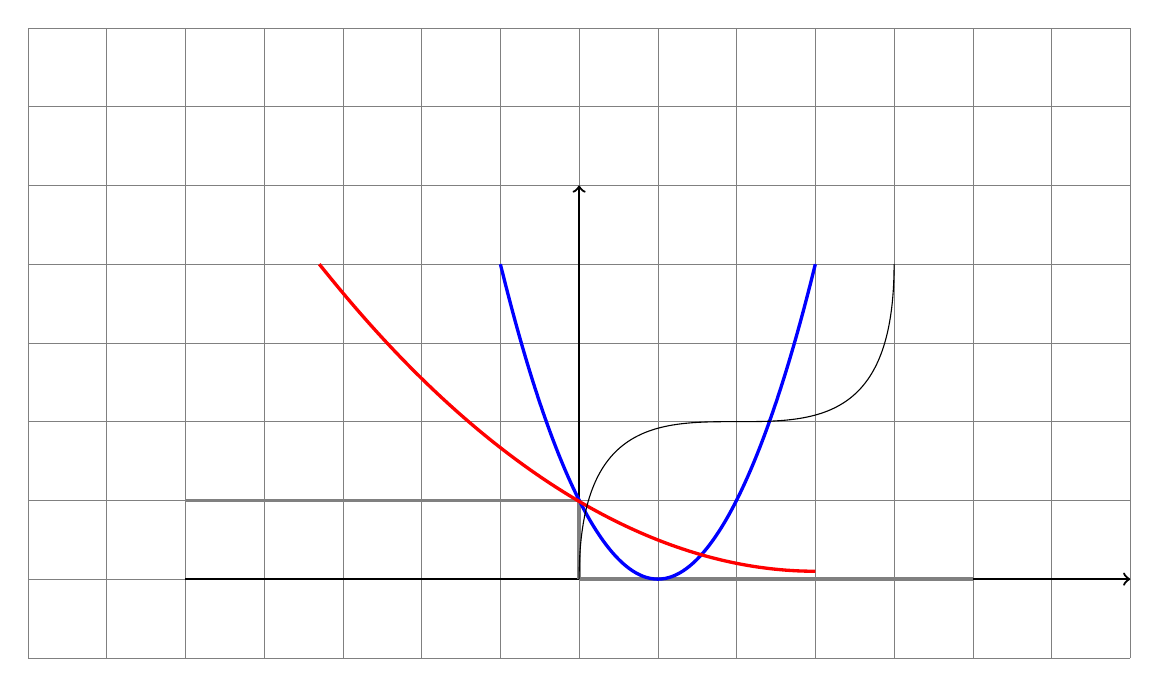
\begin{tikzpicture}		
		\draw[step=1cm,gray,very thin] (-7,-1) grid (7,7);
		\draw[thick, black, ->] (-5,0) -- (7,0);
		\draw[thick, black, ->] (0,0) -- (0,5);
		% Ideal miss-classification error		
		\draw[very thick, gray] (-5,1) -- (0,1);
		\draw[very thick, gray] (0,1) -- (0,0);
		\draw[very thick, gray] (0,0) -- (5,0);
		
		\draw[very thick, blue] (-1,4) parabola bend (1,0) (3,4);
		
		\draw[very thick, red] (3,0.1) parabola (-3.3,4);
		
		\draw (0,0) .. controls (0,4) and (4,0) .. (4,4);
		
	\end{tikzpicture}
	\caption{Different error functions: Ideal Miss-classification Error (gray line)}
\end{figure}

\section{Ideal Miss-classification Error}
Gradient = 0 $\Rightarrow$ can't use gradient descent.\\
It simply counts incorrectly classified points.

\section{Squared Error - $L_2$ Loss}
\begin{itemize}
	\item Leads to closed form solutions
	\item Sensitive to outliers
	\item Penalize "too correct" data points
\end{itemize}

\section{Cross Entropy Error}
\begin{itemize}
	\item Concave function $\Rightarrow$ unique minimum exists
	\item Robust to outliers, error increases only roughly linear
	\item No closed-form solution, requires iterative method
\end{itemize}

\section{Squared Error on Sigmoid / Tanh}
\begin{itemize}
	\item No penalty for "too correct" points
	\item Zero gradient for confidently incorrect classifications
\end{itemize}
$\Rightarrow$ \hlr{Do NOT} use $L_2$ loss with sigmoid outputs, instead, use cross-entropy.

\section{Hinge Error}
\begin{itemize}
	\item Robust to outliers
	\item Zero error for points outside margin $\Rightarrow$ sparsity
	\item Not differentiable around $z_n = 1$
\end{itemize}
\note Want the correct class to have a score that is higher than incorrect class by a fixed margin $\Delta$.
\begin{equation}
	L_i = \sum_{j \neq y_i} \text{max}(0, s_j - s_{y_i} + \Delta)
\end{equation}
in which, $s_j$ is other classes score, $s_{y_i}$ is real class score.

\section{$L_1, L_0$ Loss}
Median, no wrong points

\begin{align}
	&L_1 = \sum |t-y| \\
	&L_2 = \sum (t-y)^2
\end{align}

\section{Average Loss}
Mathematically, dividing the loss by the amount of data $N$ (in each batch or epoch) doesn't have any effect on the result. However, it's usually advisable to take the average to have more meaningful judgment and avoiding overflow when there are numerous data points.
% !TeX spellcheck = en_US
\chapter{Neural Network}
Deep neural network takes care of the complex feature engineering process (\charef{cha:feature-engineering}). \Eg, in classical computer vision, for people detection, the following process is applied:
\begin{enumerate}
	\item Input: Image
	\item Low-level feature extraction: \ac{HOG}
	\item Mid-level features: \ac{DPM}
	\item Classifier: \ac{SVM}
	\item Output: final label
\end{enumerate}
Using deep neural network, the process is truncated to simply:
\begin{enumerate}
	\item Input: Image
	\item Network training (end-to-end)
	\item Output: final label
\end{enumerate}
Different tasks require special expertise to design feature extraction, \eg, designing a program playing gammon would need someone knowing the rules, tips and tricks. On the other hands, we can assured that the human-proposed features are sufficient and helpful. Deep neural network alleviate the human-effort of hand-designing feature extraction process. In addition, it also learns prioritize important features for specific task.

\section{General}
\hlb{Forward pass:}
\begin{align}
	\textbf{y}^{(0)} &= \textbf{x}\\
	\textbf{z}^{(k)} &= \textbf{W}^{(k)}\textbf{y}^{(k-1)}, \qquad k = 1, \dots, l\\
	\textbf{y}^{(k)} &= g_k(\textbf{z}^{(k)})\\
	\textbf{y} &= \textbf{y}^{(l)}\\
	E &= L(\textbf{t}, \textbf{y}) + \lambda \Omega(\textbf{W})
\end{align}
\hlb{Backward pass:}
\begin{align}
	h \leftarrow &\frac{\partial E}{\partial \textbf{y}} = \frac{\partial}{\partial \textbf{y}} L(\textbf{t, y}) + \lambda \frac{\partial}{\partial \textbf{y}} \Omega\\
	\text{for } k =l \leftarrow &1:\\
	h \leftarrow &\frac{\partial E}{\partial \textbf{z}^{(k)}} = h \odot g(\textbf{y}^{(k)})\\
	&\frac{\partial E}{\partial \textbf{w}^{(k)}} = h \textbf{y}^{(k-1)T} + \lambda \frac{\partial \Omega}{\partial \textbf{w}^{(k)}}\\
	h \leftarrow &\frac{\partial E}{\partial \textbf{y}^{(k-1)}} = \textbf{W}^{(k)T} h
\end{align}

\section{Gradient Descent}
\note Just use ADAM??

\subsection{Vanilla Gradient Descent}
\begin{equation}
	\theta_{t+1} = \theta_t - \eta\nabla_\theta f(\theta_t)
\end{equation}
Check derivative:
\begin{equation}
	f'(x) \approx \frac{f(x+\varepsilon) - f(x-\varepsilon)}{2\varepsilon} \;\;\;\;\; \text{(numerical gradient)}
\end{equation}

\subsection{Momentum}
\begin{itemize}
	\item Init: $v_{dW_0} = 0, v_{db_0} = 0$
	\item Calculate $dW, db$
	\item Update $W, b$
	\begin{equation}
		\Rightarrow \begin{cases}
			v_{dW} &= \beta v_{dW} + (1-\beta)dW\\
			v_{db} &= \beta v_{db} + (1-\beta)db
		\end{cases}
		\Rightarrow
		\begin{cases}
			W &= W - \alpha v_{dW}\\
			b &= b - \alpha v_{db}
		\end{cases}
	\end{equation}
	The above formulas are to calculate the moving average of $v_{dW}$ and $v_{db}$.
	\item Tips: Choose \hlre{\beta_1=0.9}, implying taking average of the last 10 steps.
	\item Reference source: \href{https://youtu.be/k8fTYJPd3_I}{DeepLearning.AI}.
\end{itemize}

\subsection{Nesterov Accelerated Gradient}
\ac{nag}:
\begin{equation}
	v_t = \gamma v_{t-1} + \eta \nabla_tJ\left(\theta - \gamma v_{t-1}\right)
\end{equation}

\subsection{\ac{rmsprop}}
\begin{itemize}
	\item Init $s_{dW_0} = 0, s_{db_0}=0$
	\item Calculate $dW, db$
	\item Update $W, b$
	\begin{equation}
		\begin{cases}
			s_{dW} &= \beta s_{dW} + (1-\beta)dW^2 \\
			s_{db} &= \beta s_{db} + (1-\beta)db^2
		\end{cases}
		\Rightarrow
		\begin{cases}
			W &= W - \alpha \frac{dW}{\sqrt{s_{dW}} + \varepsilon}\\
			b &= b - \alpha \frac{db}{\sqrt{s_{db}} + \varepsilon}
		\end{cases}
	\end{equation}
	\item Tips: choose \hlre{\beta_2 = 0.999, \;\;\varepsilon = 10^{-7}}
	\item Reference source: \href{https://youtu.be/_e-LFe_igno}{DeepLearning.AI}.
\end{itemize}

\subsection{\ac{adam}}
\ac{adam} is basically the combination of Momentum and \ac{rmsprop}.
\begin{itemize}
	\item Init $v_{dW_0}, s_{dW_0}, v_{db_0}, s_{db_0}=0$
	\item Calculate $dW, db$
	\item Update $W, b$
	\begin{equation}
		\begin{cases}
			v_{dW} &= \beta_1 v_{dW} + (1-\beta_1)dW \\
			v_{db} &= \beta_1 v_{db} + (1-\beta_1)db \\
			s_{dW} &= \beta_2 s_{dW} + (1-\beta_2)dW^2 \\
			s_{db} &= \beta_2 s_{db} + (1-\beta_2)db^2
		\end{cases}
		\Rightarrow
		\begin{cases}
			v^{cor.}_{dW} &= \frac{v_{dW}}{1 - \beta_1^t} \\
			v^{cor.}_{db} &= \frac{v_{db}}{1 - \beta_1^t} \\
			s^{cor.}_{dW} &= \frac{s_{dW}}{1 - \beta_2^t} \\
			s^{cor.}_{db} &= \frac{s_{db}}{1 - \beta_2^t}
		\end{cases}
		\Rightarrow
		\begin{cases}
			W &= W - \alpha \frac{v^{cor.}_{dW}}{\sqrt{s^{cor.}_{dW}} + \varepsilon}\\
			b &= b - \alpha \frac{v^{cor.}_{db}}{\sqrt{s^{cor.}_{db}} + \varepsilon}
		\end{cases}
	\end{equation}
	\item Tips: choose \hlre{\beta_1 = 0.9, \quad\beta_2 = 0.999, \quad\varepsilon = 10^{-7}}
	\item Reference source: \href{https://youtu.be/JXQT_vxqwIs}{DeepLearning.AI}.
\end{itemize}

\section{Convolutional Operator}
\subsection{Convolution}
\cite{lecun1998gradient}

\subsection{Transposed Convolution}
This module can be seen as the gradient of Conv2d with respect to its input. It is also known as a fractionally-strided convolution or a deconvolution (although it is not an actual deconvolution operation as it does not compute a true inverse of convolution). For more information, see the visualizations here \cite{dumoulin2016guide} and the Deconvolutional Networks paper \cite{zeiler2010deconvolutional}.

\section{Tips and Tricks}
\begin{itemize}
	\item Shuffling
	\item Data Augmentation: reshape, rescale, crops, zooming, change color (color \ac{PCA})
	\item Normalizing the inputs\\
	Convergence is the fastest if
	\begin{itemize}
		\item The mean of each input variable $=0$
		\item Scale $\Rightarrow$ same covariance
	\end{itemize}
	Mean cancellation $\Rightarrow$ \ac{KL} expansion $\Rightarrow$ covariance equalization (if possible)
	\item Leaky \ac{relu} is better a bit than \ac{relu}, ELU
	\item Weights initialization: Xavier-Glorot:
	\[ W \sim U\left(0, \sqrt{\frac{6}{n_{in} + n_{out}}}\right) \]
	\item Batch Norm(alization): Normalize after each layer\\
	$\Rightarrow$ learn the moving average
	\item Drop out\\
	\note When in inferencing (after training), must multiply the activation output with the \ac{prob} that the weights are set to 0
\end{itemize}
% !TeX spellcheck = en_US
\chapter{Network Structures}
This chapter presents some common network structures and their capabilities.

\section{Base Structures}
\subsection{LeNet}
LeNet5 is probably the earliest \ac{CNN} network, proposed by \citeausm{lecun1998gradient}.

\begin{figure}[hbt!]
	\centering
	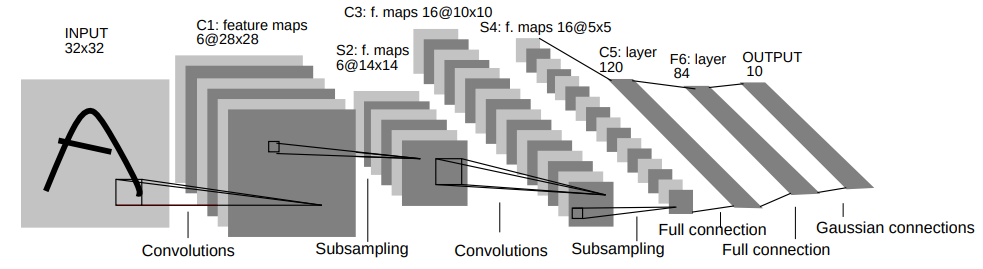
\includegraphics[width=\textwidth]{lenet.png}
	\caption{LeNet5 Architecture. \cite{lecun1998gradient}}
\end{figure}

Example coding with \texttt{pytorch} (\href{https://blog.paperspace.com/writing-lenet5-from-scratch-in-python/}{src}):
\begin{python}
import torch.nn as nn
	
class LeNet5(nn.Module):
	def __init__(self, num_classes):
		super(ConvNeuralNet, self).__init__()
		self.conv1 = nn.Sequential(
		nn.Conv2d(1, 6, kernel_size=5, stride=1, padding=0),
		nn.BatchNorm2d(6),
		nn.ReLU(),
		nn.MaxPool2d(kernel_size = 2, stride = 2))
		self.conv2 = nn.Sequential(
		nn.Conv2d(6, 16, kernel_size=5, stride=1, padding=0),
		nn.BatchNorm2d(16),
		nn.ReLU(),
		nn.MaxPool2d(kernel_size = 2, stride = 2))
		self.fc1 = nn.Sequential(
		nn.Linear(400, 120),
		nn.ReLU())
		self.fc2 = nn.Sequential(
		nn.Linear(120, 84),
		nn.ReLU())
		self.fc3 = nn.Linear(84, num_classes)
	
	def forward(self, x):
		...
		return y
\end{python}

\subsection{AlexNet}
The classic \ac{CNN} architecture for image classification on the CIFAR10 dataset \cite{krizhevsky2012imagenet}.

\begin{figure}[hbt!]
	\centering
	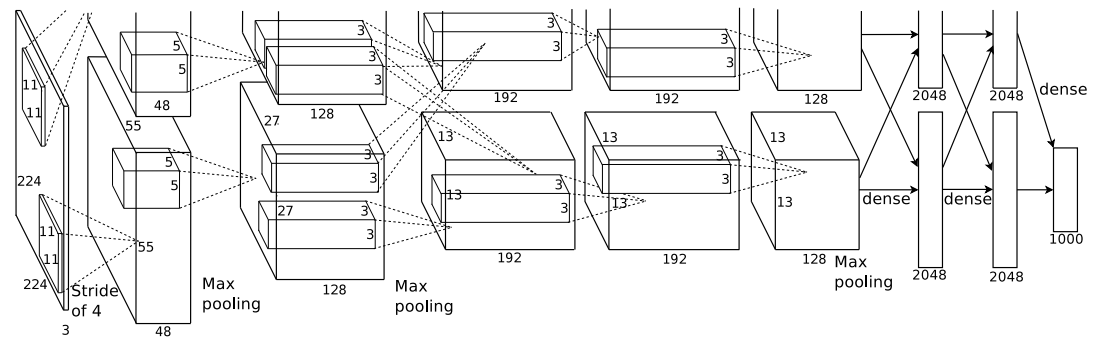
\includegraphics[width=\textwidth]{alexnet.png}
	\caption{AlexNet architecture. \cite{krizhevsky2012imagenet}}
\end{figure}

Example coding with \texttt{pytorch} (\href{https://blog.paperspace.com/alexnet-pytorch/}{src}):
\begin{python}	
class AlexNet(nn.Module):
	def __init__(self, num_classes=10):
		super(AlexNet, self).__init__()
		self.layer1 = nn.Sequential(
		nn.Conv2d(3, 96, kernel_size=11, stride=4, padding=0),
		nn.BatchNorm2d(96),
		nn.ReLU(),
		nn.MaxPool2d(kernel_size = 3, stride = 2))
		...
		self.fc1 = nn.Sequential(
		nn.Dropout(0.5),
		nn.Linear(4096, 4096),
		nn.ReLU())
		self.fc2= nn.Sequential(
		nn.Linear(4096, num_classes))
	
	def forward(self, x):
		...
		return y
\end{python}

\subsection{VGG Net}
The runner-up at the ILSVRC 2014 competition by \citeaus{simonyan2014very}:

\begin{figure}[hbt!]
	\centering
	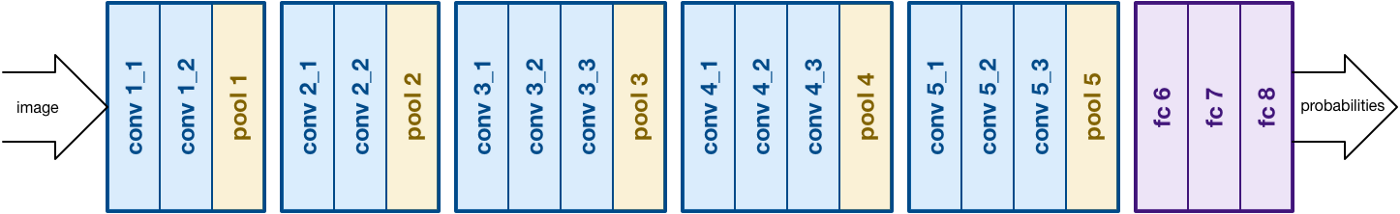
\includegraphics[width=\textwidth]{vggnet.png}
	\caption{The VGG Net architecture with 13 \ac{CONV} layers and 3 \ac{FC} layers. \cite{simonyan2014very}}
\end{figure}

Example coding with \texttt{pytorch} (\href{https://blog.paperspace.com/vgg-from-scratch-pytorch/}{src}):
\begin{python}
	class VGG16(nn.Module):
	def __init__(self, num_classes=10):
	super(VGG16, self).__init__()
	self.layer1 = nn.Sequential(
	nn.Conv2d(3, 64, kernel_size=3, stride=1, padding=1),
	nn.BatchNorm2d(64),
	nn.ReLU())
	...
	self.fc1 = nn.Sequential(
	nn.Dropout(0.5),
	nn.Linear(4096, 4096),
	nn.ReLU())
	self.fc2= nn.Sequential(
	nn.Linear(4096, num_classes))
	
	def forward(self, x):
	...
	return y
\end{python}

\subsection{Residual Network}
The \ac{ResNet} by \citeausm{he2016deep} tackles the vanishing gradient problem for deep neural network with the residual block (\figref{fig:residual-modul}). It creates a highway pass for the gradient to go to the early layers.
\begin{figure}[hbt!]
	\centering
	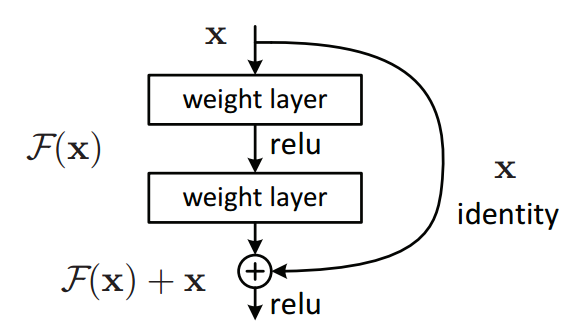
\includegraphics[width=0.5\textwidth]{residual-modul.png}
	\caption{Residual block \cite{he2016deep}.}
	\label{fig:residual-modul}
\end{figure}

Example coding with \texttt{pytorch} (\href{https://blog.paperspace.com/writing-resnet-from-scratch-in-pytorch/}{src}):
\begin{python}
class ResidualBlock(nn.Module):
	def __init__(self, in_channels, out_channels,
			stride = 1, downsample = None):
		super(ResidualBlock, self).__init__()
		self.conv1 = nn.Sequential(
		nn.Conv2d(in_channels, out_channels, kernel_size = 3,
		stride = stride, padding = 1),
		nn.BatchNorm2d(out_channels),
		nn.ReLU())
		self.conv2 = nn.Sequential(
		nn.Conv2d(out_channels, out_channels, kernel_size = 3,
		stride = 1, padding = 1),
		nn.BatchNorm2d(out_channels))
		self.downsample = downsample
		self.relu = nn.ReLU()
		self.out_channels = out_channels
	
	def forward(self, x):
		residual = x
		out = self.conv1(x)
		out = self.conv2(out)
		if self.downsample:
			residual = self.downsample(x)
		out += residual
		out = self.relu(out)
		return out
\end{python}

\begin{python}
class ResNet(nn.Module):
	def __init__(self, block, layers, num_classes = 10):
		super(ResNet, self).__init__()
		self.inplanes = 64
		self.conv1 = nn.Sequential(
		nn.Conv2d(3, 64, kernel_size = 7, stride = 2, padding = 3),
		nn.BatchNorm2d(64),
		nn.ReLU())
		self.maxpool = nn.MaxPool2d(kernel_size = 3, stride = 2, padding = 1)
		self.layer0 = self._make_layer(block, 64, layers[0], stride = 1)
		self.layer1 = self._make_layer(block, 128, layers[1], stride = 2)
		self.layer2 = self._make_layer(block, 256, layers[2], stride = 2)
		self.layer3 = self._make_layer(block, 512, layers[3], stride = 2)
		self.avgpool = nn.AvgPool2d(7, stride=1)
		self.fc = nn.Linear(512, num_classes)
		
	def _make_layer(self, block, planes, blocks, stride=1):
		downsample = None
		if stride != 1 or self.inplanes != planes:
			downsample = nn.Sequential(
				nn.Conv2d(self.inplanes, planes, kernel_size=1, stride=stride),
				nn.BatchNorm2d(planes),
				)
		layers = []
		layers.append(block(self.inplanes, planes, stride, downsample))
		self.inplanes = planes
		for i in range(1, blocks):
			layers.append(block(self.inplanes, planes))
		return nn.Sequential(*layers)
	
	def forward(self, x):
		x = self.conv1(x)
		x = self.maxpool(x)
		x = self.layer0(x)
		x = self.layer1(x)
		x = self.layer2(x)
		x = self.layer3(x)
		x = self.avgpool(x)
		x = x.view(x.size(0), -1)
		x = self.fc(x)
		return x
	
model = ResNet(ResidualBlock, [3, 4, 6, 3]).to(device)
\end{python}

\subsection{GoogLeNet}
\todo{}

\subsection{U-Net}
The U-Net architecture by \citeaus{ronneberger2015u} can also be viewed as an encoder-decoder architecture \cite{kingma2013auto} with skip connections of \texttt{ResNet} (\figref{fig:unet1}). This structure is later adopted in \texttt{pix2pix} architecture for image-to-image translation \cite{isola2017image}.
\begin{figure}[hbt!]
	\centering
	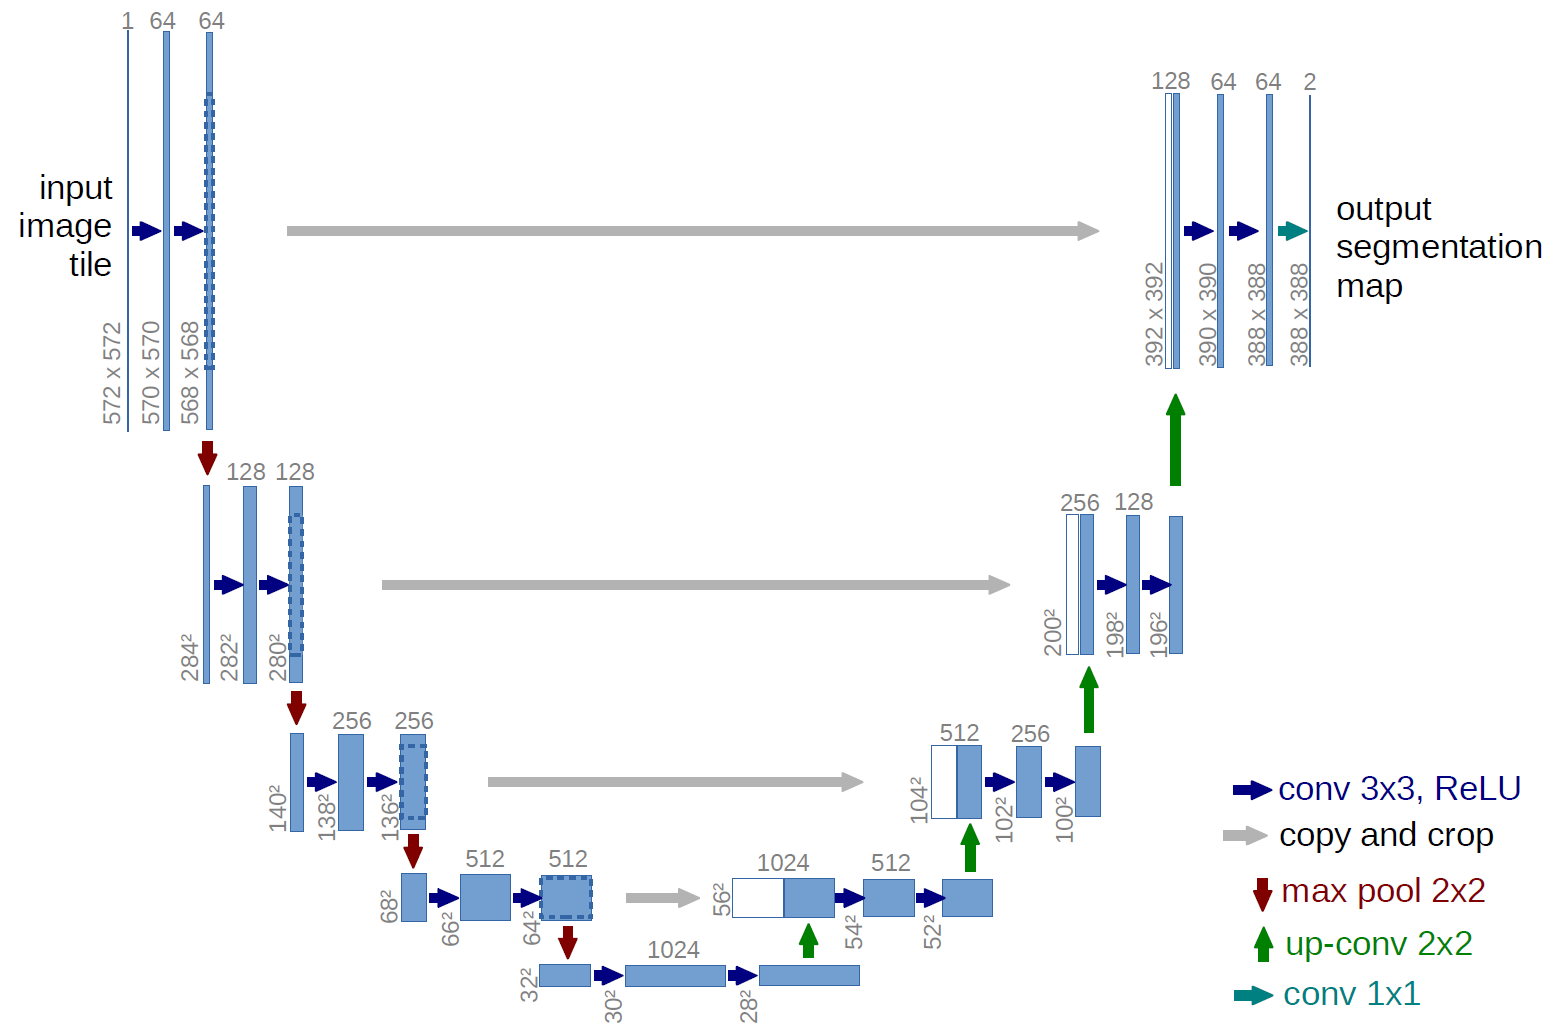
\includegraphics[width=0.9\textwidth]{unet.png}
	\caption{The U-Net architecture. \cite{ronneberger2015u}}
\end{figure}
\begin{figure}[hbt!]
	\centering
	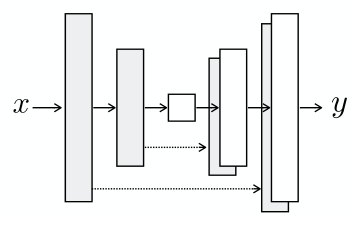
\includegraphics[width=0.35\textwidth]{unet1.png}
	\caption{The U-Net as a variational auto-encoder with skip connections. \cite{isola2017image}}
	\label{fig:unet1}
\end{figure}

\todo{benefits, comments?}

\subsection{DenseNet}
\todo{} \citeaustitle{huang2017densely}

\subsection{Comparison between Networks}
\begin{figure}[hbt!]
	\centering
	\begin{minipage}{.5\textwidth}
		\centering
		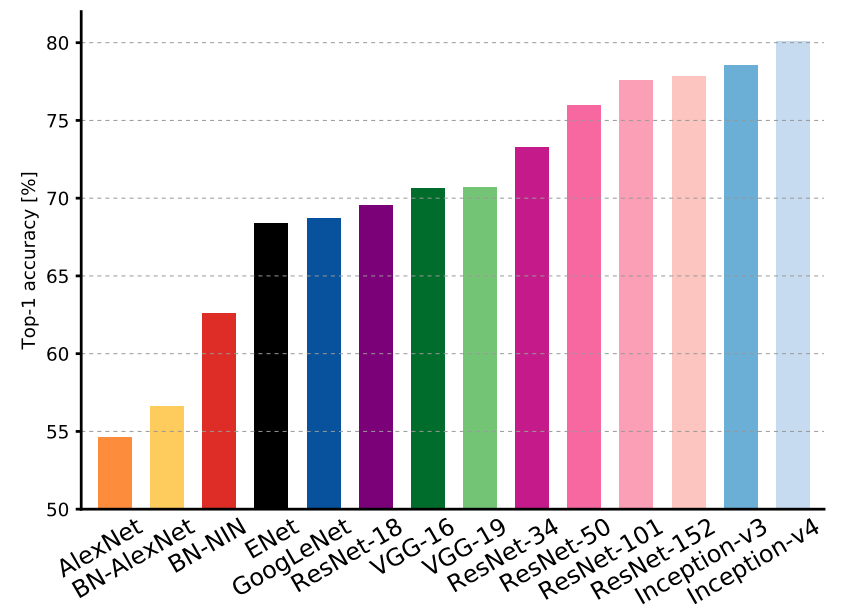
\includegraphics[width=0.95\textwidth]{top1accuracy-nets.png}
		\captionof{figure}{Top1 \ac{vs} network.}
		\label{fig:top1accuracy-nets}
	\end{minipage}%
	\begin{minipage}{.5\textwidth}
		\centering
		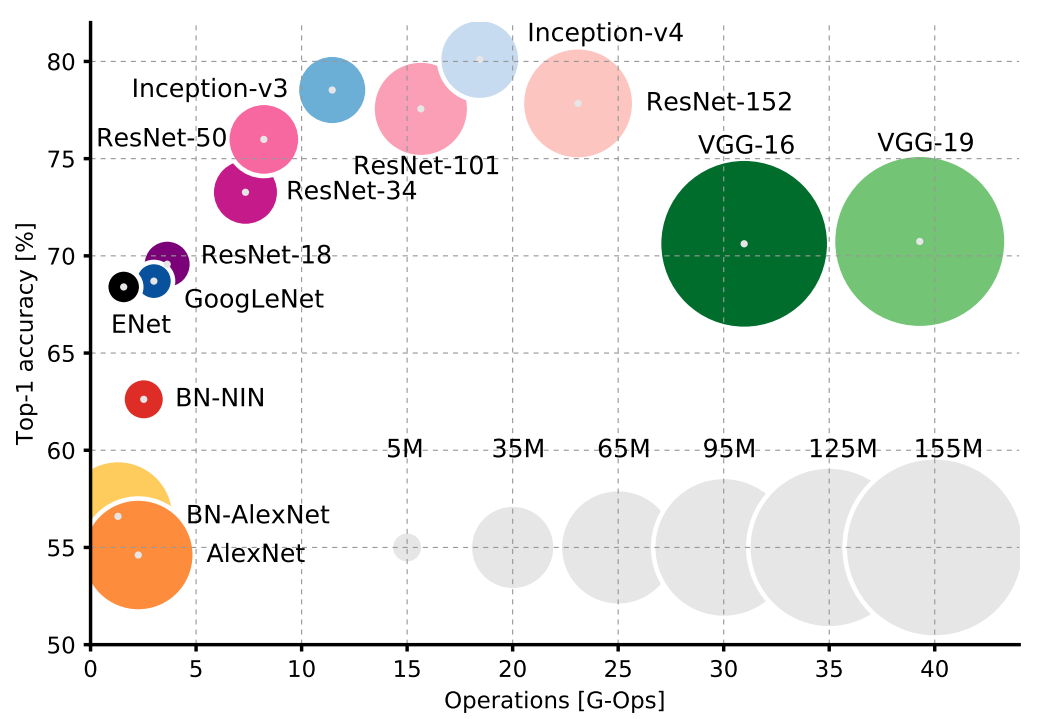
\includegraphics[width=0.95\textwidth]{top1accuracy-size-nets.png}
		\captionof{figure}{Top1 \ac{vs} operations, size $\propto$ \ac{param}.}
		\label{fig:top1accuracy-size-nets}
	\end{minipage}
\end{figure}

\section{Structures for Sequential Data}
\subsection{Recurrent Neural Network}
The next three models deal with sequential data. It's a bit uncertain what is the original paper proposing the idea though \cite{elman1990finding}. \ac{BPTT}:\\
\todo{Add image, content}
\begin{align}
	\frac{\partial E_t}{\partial w_{ij}} &= \sum_{1 \leq k \leq t} \left( \frac{\partial E_t}{\partial h_t} \frac{\partial h_t}{\partial h_k} \frac{\partial h_k}{\partial w_{ij}} \right)\\
	E &= \sum_{1 \leq t \leq T} E_t\\
	\frac{\partial h_t}{\partial h_k} &= \prod_{t \geq i \geq k} \frac{\partial h_i}{\partial h_{i-1}}
\end{align}

\subsection{LSTM}
\cite{sutskever2014sequence} \todo{}

\subsection{Transformer}
\ac{RNN} suffers from vanishing/exploding gradient. \ac{LSTM} suffers from slow training time. \citeausm{vaswani2017attention} propose a approach based on the idea of attention. This approach can utilize the computation power of \ac{GPU} for parallelized matrix computation. This technique originally is meant for \ac{NLP} problem, but later on, also show meaningful application in \ac{CV}.

\begin{itemize}
	\item A easy and detailed explanation from \citeaus{alammar2020}
	This idea is the basis for GPT-3 \cite{brown2020language} and BERT \cite{devlin2018bert}
\end{itemize}
\begin{figure}[hbt!]
	\centering
	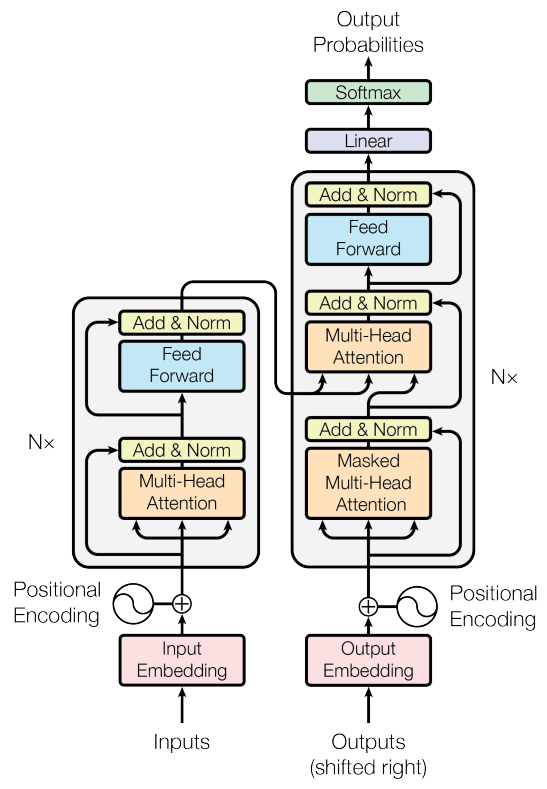
\includegraphics[width=0.5\textwidth]{transformer.png}
	\caption{The Transformer - model architecture \cite{vaswani2017attention}.}
\end{figure}

\begin{figure}[hbt!]
	\centering
	\begin{minipage}{.5\textwidth}
		\centering
		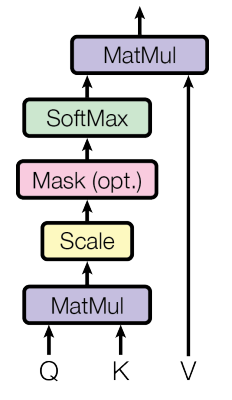
\includegraphics[width=0.55\textwidth]{transformer-1.png}
		\captionof{figure}{Scaled Dot-Product Attention.}
	\end{minipage}%
	\begin{minipage}{.45\textwidth}
		\centering
		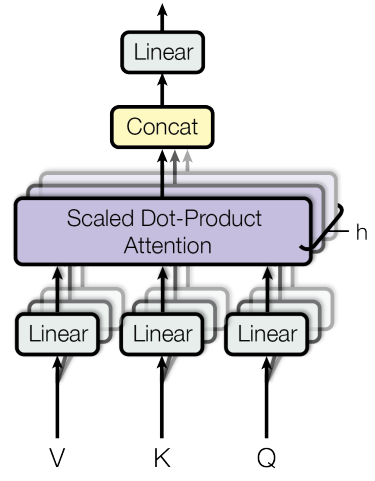
\includegraphics[width=0.82\textwidth]{transformer-2.png}
		\captionof{figure}{Multi-Head Attention.}
	\end{minipage}
\end{figure}

\section{Bayesian Neural Network}
Deep neural network's strength is its ability to approximate function. However, as powerful as it is, there is also a threat to overfit to the training data and fail to generalize on the test set. There are various techniques to reduce overfit and improve transfer learning, \eg, weight regularization, dropout, batch norm.

A conventional neural network takes in the same input and produce the same output. A Bayesian neural network different output when it takes in the same inputs twice. The resulting algorithm:
\begin{itemize}
	\item mitigates overfitting
	\item enables learning from small datasets
	\item tells us how uncertain our predictions are.
	\item adds stochasticity to neural network.
	\item Instead of weights, it has weights with distribution
	\begin{align}
		w_i \sim \mathcal{N}(\mu_i, \sigma_i^2)
	\end{align}
\end{itemize}

\note There is a thing called Bayesian Network, \ac{aka} belief network, which is not the same as Bayesian neural network.

\begin{align*}
	\mathcal{D}_{tr} = \{\textbf{x}_i, y_i\}^n_{i=1}, \quad \text{model } F_\theta, \quad \text{loss } \mathcal{L}
\end{align*}
\begin{center}
	\begin{tabular}{p{7cm}|p{8cm}}
		Neural Network & Bayesian Neural Network\\ \hline \hline
		Training:
		\[\theta^* = \underset{\theta}{\arg\max} \sum_{(\textbf{x}_i, y_i)} \log [p(y_i | \textbf{x}_i, \theta)]\]
		\[\theta^* = \underset{\theta}{\arg\min} \sum_{(\textbf{x}_i, y_i)} \mathcal{L}(F_\theta(\textbf{x}_i), y_i)\] & Training:
		\[\mu^*, \Sigma^* = \underset{\mu, \Sigma}{\arg\max} \sum_{(\textbf{x}_i, y_i)} \log [p(y_i | \textbf{x}_i, \theta)] - KL[p(\theta), p(\theta_0)] \]
		\[\theta \sim \mathcal{N}(\mu, \Sigma), \qquad \theta_0 \sim \mathcal{N}(\textbf{0, I})\]
		\[\mu^*, \Sigma^* = \underset{\mu, \Sigma}{\arg\min} \sum_{(\textbf{x}_i, y_i)} \mathcal{L}(F_\theta(\textbf{x}_i), y_i) + KL[p(\theta), p(\theta_0)] \]
		\\ \hline
		Prediction:
		\[p(\hat{y} | \hat{\textbf{x}}, \theta^*)\]
		\[\hat{y} = F_{\theta^*}(\hat{\textbf{x}})\] & Prediction:
		\[p(\hat{y} | \hat{\textbf{x}}, \mathcal{D}_{tr}) = \int p(\hat{y} | \hat{\textbf{x}}, \theta^*) p(\theta^* | \mathcal{D}_{tr}) d\theta^* \]
		\[\theta^* \sim \mathcal{N}(\mu^*, \Sigma^*)\]
		\[\hat{y} = \frac{1}{K} \sum_{k=1}^K F_{\theta^*_k} (\hat{\textbf{x}}), \qquad \theta^*_k \sim \mathcal{N}(\mu^*, \Sigma^*)\]
	\end{tabular}
\end{center}

\subsection{References}
Examples:
\begin{itemize}
	\item \href{https://www.cs.toronto.edu/~duvenaud/distill_bayes_net/public/}{cs.toronto}
	\item \href{https://keras.io/examples/keras_recipes/bayesian_neural_networks/}{Keras's example}
	\item \href{https://github.com/Harry24k/bayesian-neural-network-pytorch}{BNN-pytorch}
	\item \href{https://github.com/kumar-shridhar/PyTorch-BayesianCNN}{PyTorch-BayesianCNN}
\end{itemize}

If you want to just get the high level idea, watch these:
\begin{itemize}
	\item \href{https://youtu.be/s0S6HFdPtlA}{YouTube/PyData}
\end{itemize}

References: \note very long and complicate papers, I don't read them
\begin{itemize}
	\item \citeaustitle{jospin2022hands}
	\item \citeaustitle{shridhar2019comprehensive}
	\item \citeaustitle{liu2018adv}
\end{itemize}

\section{Graph Neural Networks}
\subsection{Introduction}
Many systems and interactions can be represented as graphs. \ac{GNN} are neural networks that operate on graph-structured data. Examples:

\begin{figure}[hbt!]
	\centering
	\begin{minipage}{.47\textwidth}
		\centering
		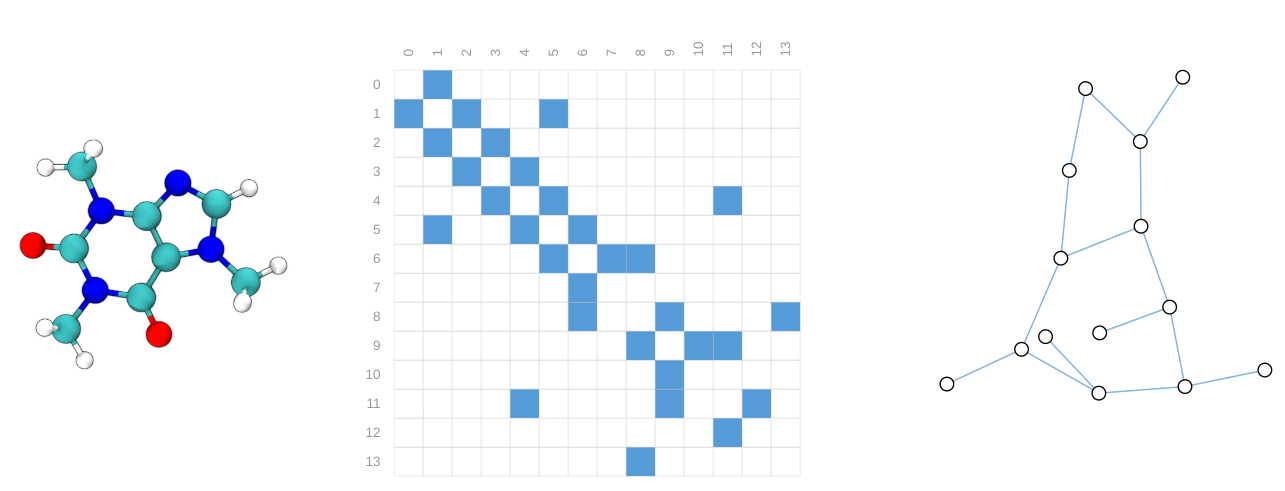
\includegraphics[width=\textwidth]{molecule-gnn.png}
		\captionof{figure}{Caffeine molecule structure as a graph. \cite{sanchez2021a}}
	\end{minipage}
	\hfil
	\begin{minipage}{.47\textwidth}
		\centering
		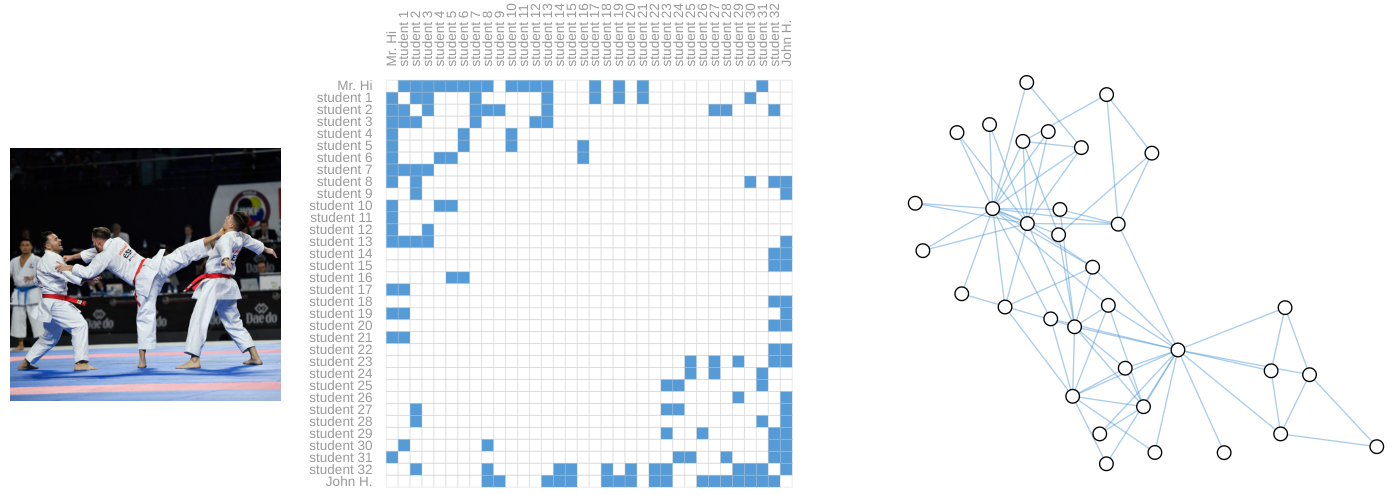
\includegraphics[width=\textwidth]{social-network-gnn.png}
		\captionof{figure}{A social network as a graph. \cite{sanchez2021a}}
	\end{minipage}
\end{figure}

Image and text can also be modeled as graphs, but it would be redundant, since they have fixed structures. Pixels in image are connected in a grid and words in a sentence are connected only with the prior and next ones.

There are three general types of prediction tasks on graphs: \cite{sanchez2021a}
\begin{itemize}
	\item graph-level: predict a single property for a whole graph. This is analogous to classification / regression problem on MNIST or CIFAR datasets.\\
	\Eg: Given a graph representing a molecule, predict the smell of it.
	\item node-level: predict some property for each node in a graph. This is analogous to segmentation problem of \ac{CV}, in which we predict the class for each pixel.\\
	\Eg: Given a graph representing the social network, predict the famous score of a person (a node)
	\item edge-level: predict the property or presence of edges in a graph.\\
	\Eg: Given a image of different peoples, objects, predict the interactions between them (\figref{fig:edge-level-task-GNN})
\end{itemize}

There are also
\begin{itemize}
	\item Node clustering task
	\item Link Prediction: Predicting missing links.
	\item Influence Maximization: Identifying influential nodes.
\end{itemize}

\begin{figure}[hbt!]
	\centering
	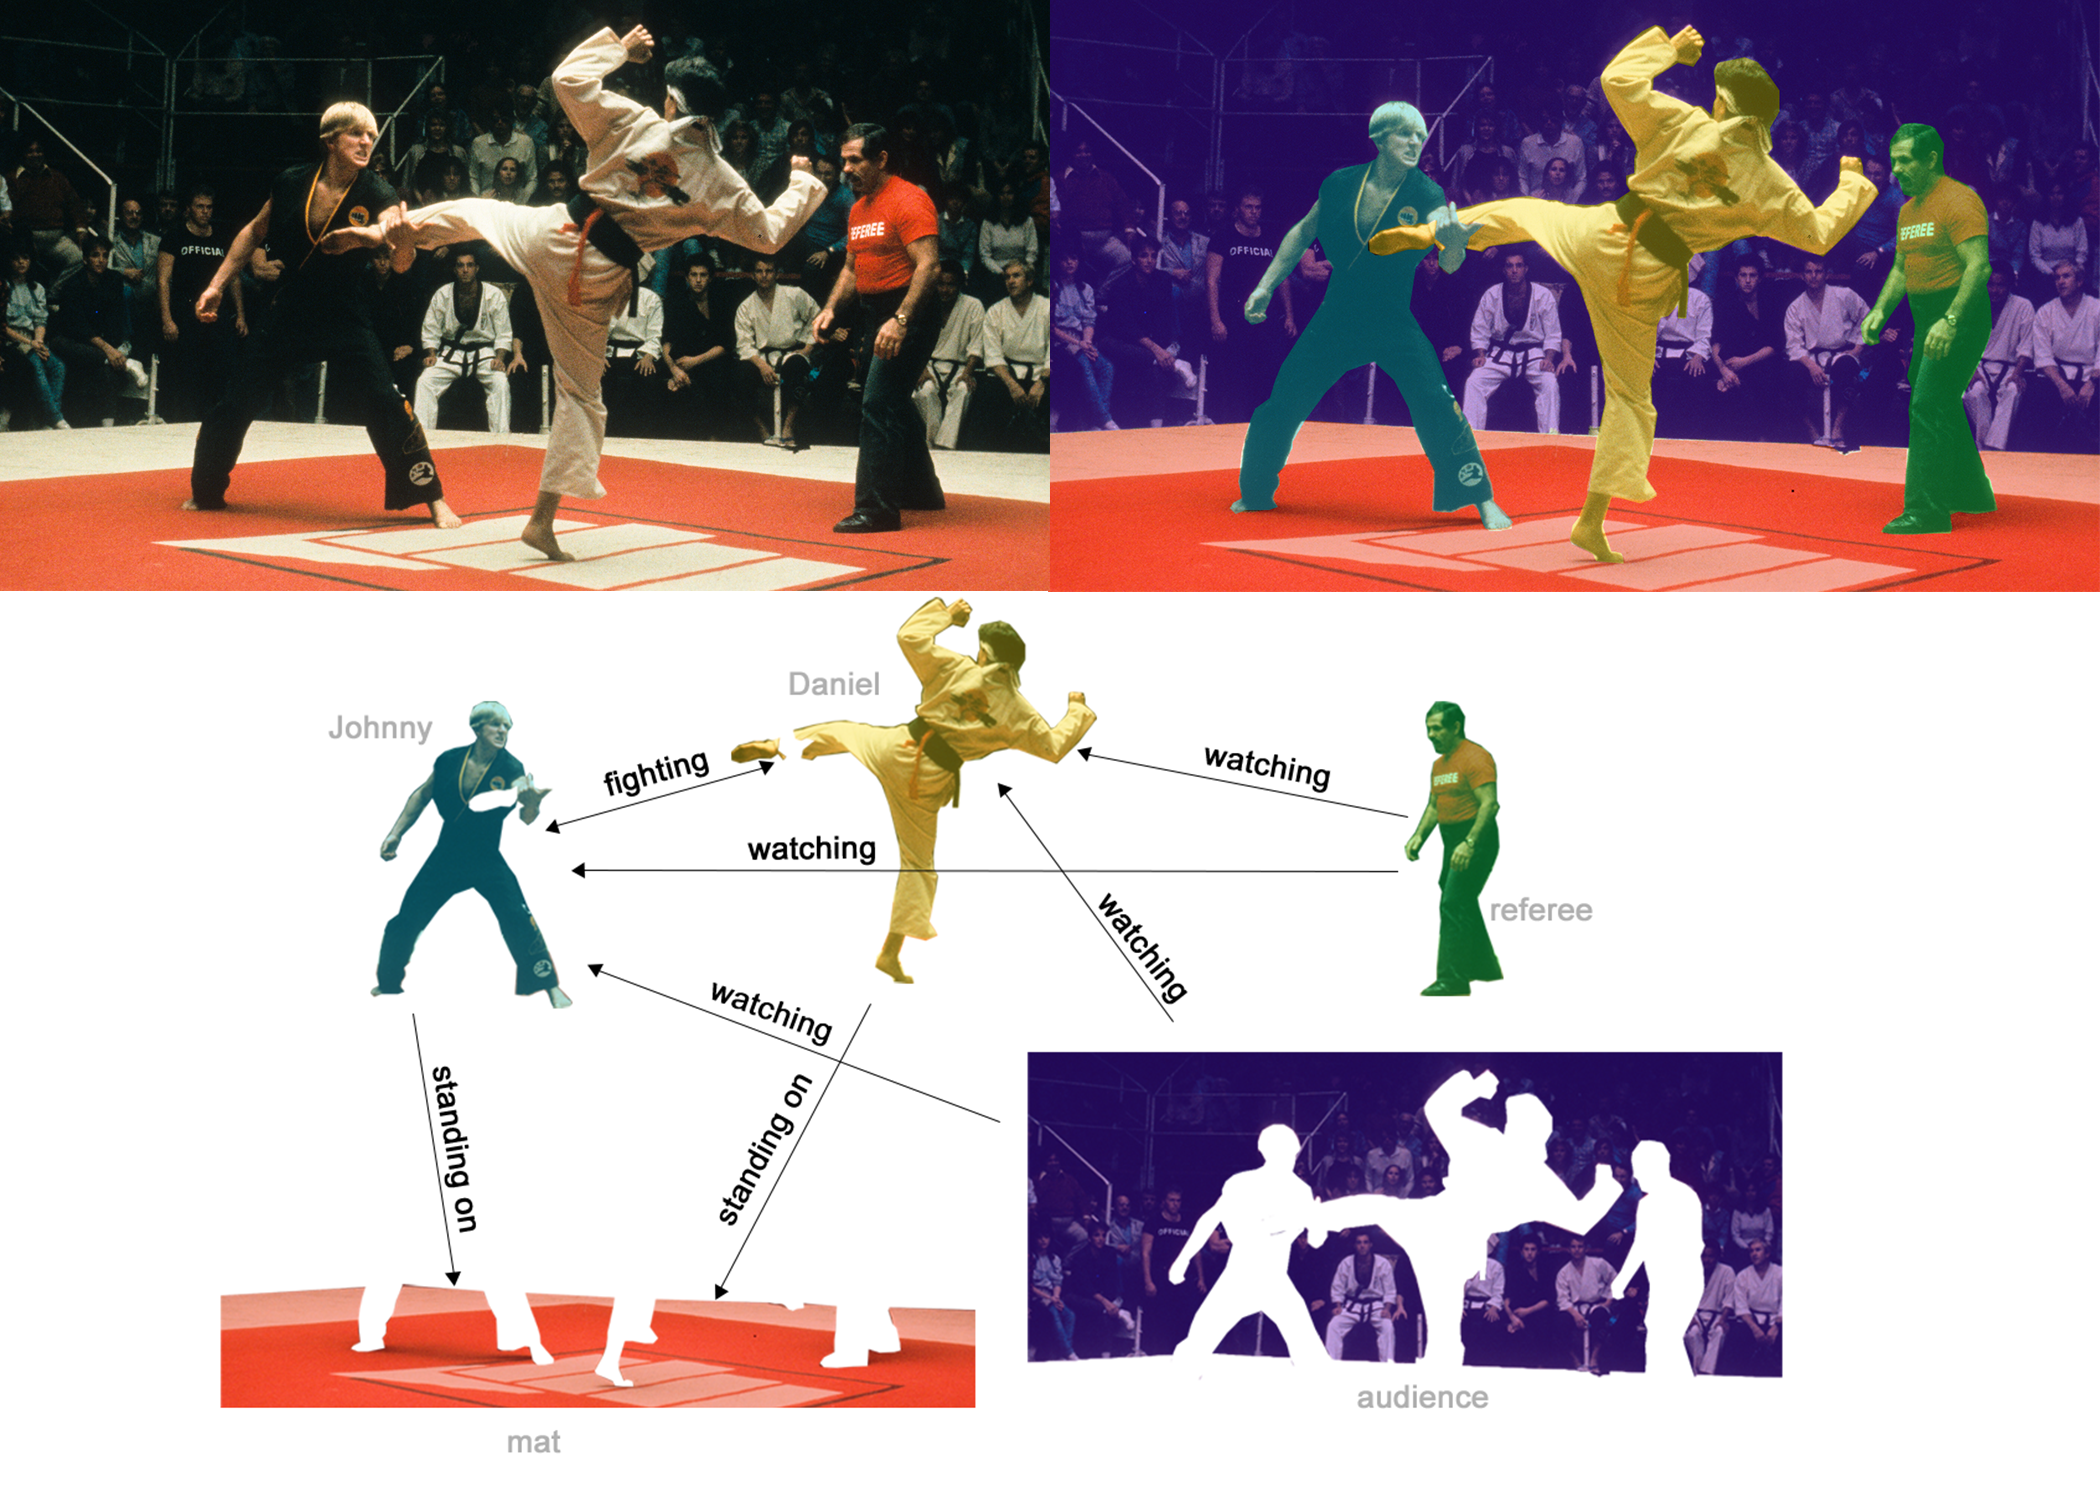
\includegraphics[width=0.79\textwidth]{edge-level-task-GNN.png}
	\caption{Example of edge-level prediction task \cite{sanchez2021a}.}
	\label{fig:edge-level-task-GNN}
\end{figure}

\subsection{Challenges}
\note Batch learning is difficult the setup

\subsection{Graph Representations in Machine Learning}
\begin{itemize}
	\item Using adjacency matrix is not permutation-invariant. (\figref{fig:graph-permutation})
	\begin{figure}[hbt!]
		\centering
		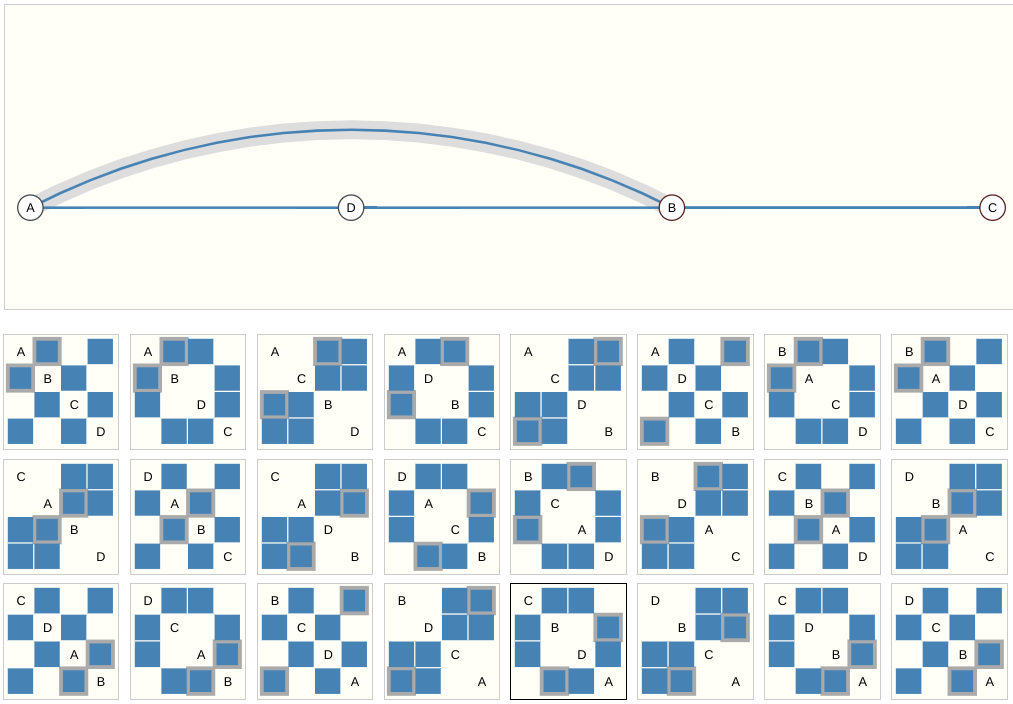
\includegraphics[width=0.79\textwidth]{graph-permutation.png}
		\caption{Different adjacency matrices represent the same graph \cite{sanchez2021a}.}
		\label{fig:graph-permutation}
	\end{figure}
	\item Another option is adjacency list
	\begin{itemize}
		\item Nodes: list of feature vectors for each node, tensor size $[n_{nodes}, dim_{node}]$
		\item Edges: list of feature vectors for each edge, tensor size $[n_{edges}, dim_{edge}]$
		\item Adjacency list: list of edges, tensor size $[n_{edges}, 2]$
		\item Global: a single feature vectors for global value, tensor size $[1, dim_{global}]$
	\end{itemize}
	\item Feature vector is also called as representation or embedding
	\Eg: feature vector for a person node in a social network: $\begin{bmatrix}
		age\\
		job\\
		marriage\ status\\
		nationality\\
		location
	\end{bmatrix}$
\end{itemize}

\subsection{GNN Block}
Between layers in \ac{GNN}, there are 3 \ac{MLP} to update graph attributes: feature vectors of nodes, edges and global value. \note The adjacency list stays unchanged.
\begin{figure}[hbt!]
	\centering
	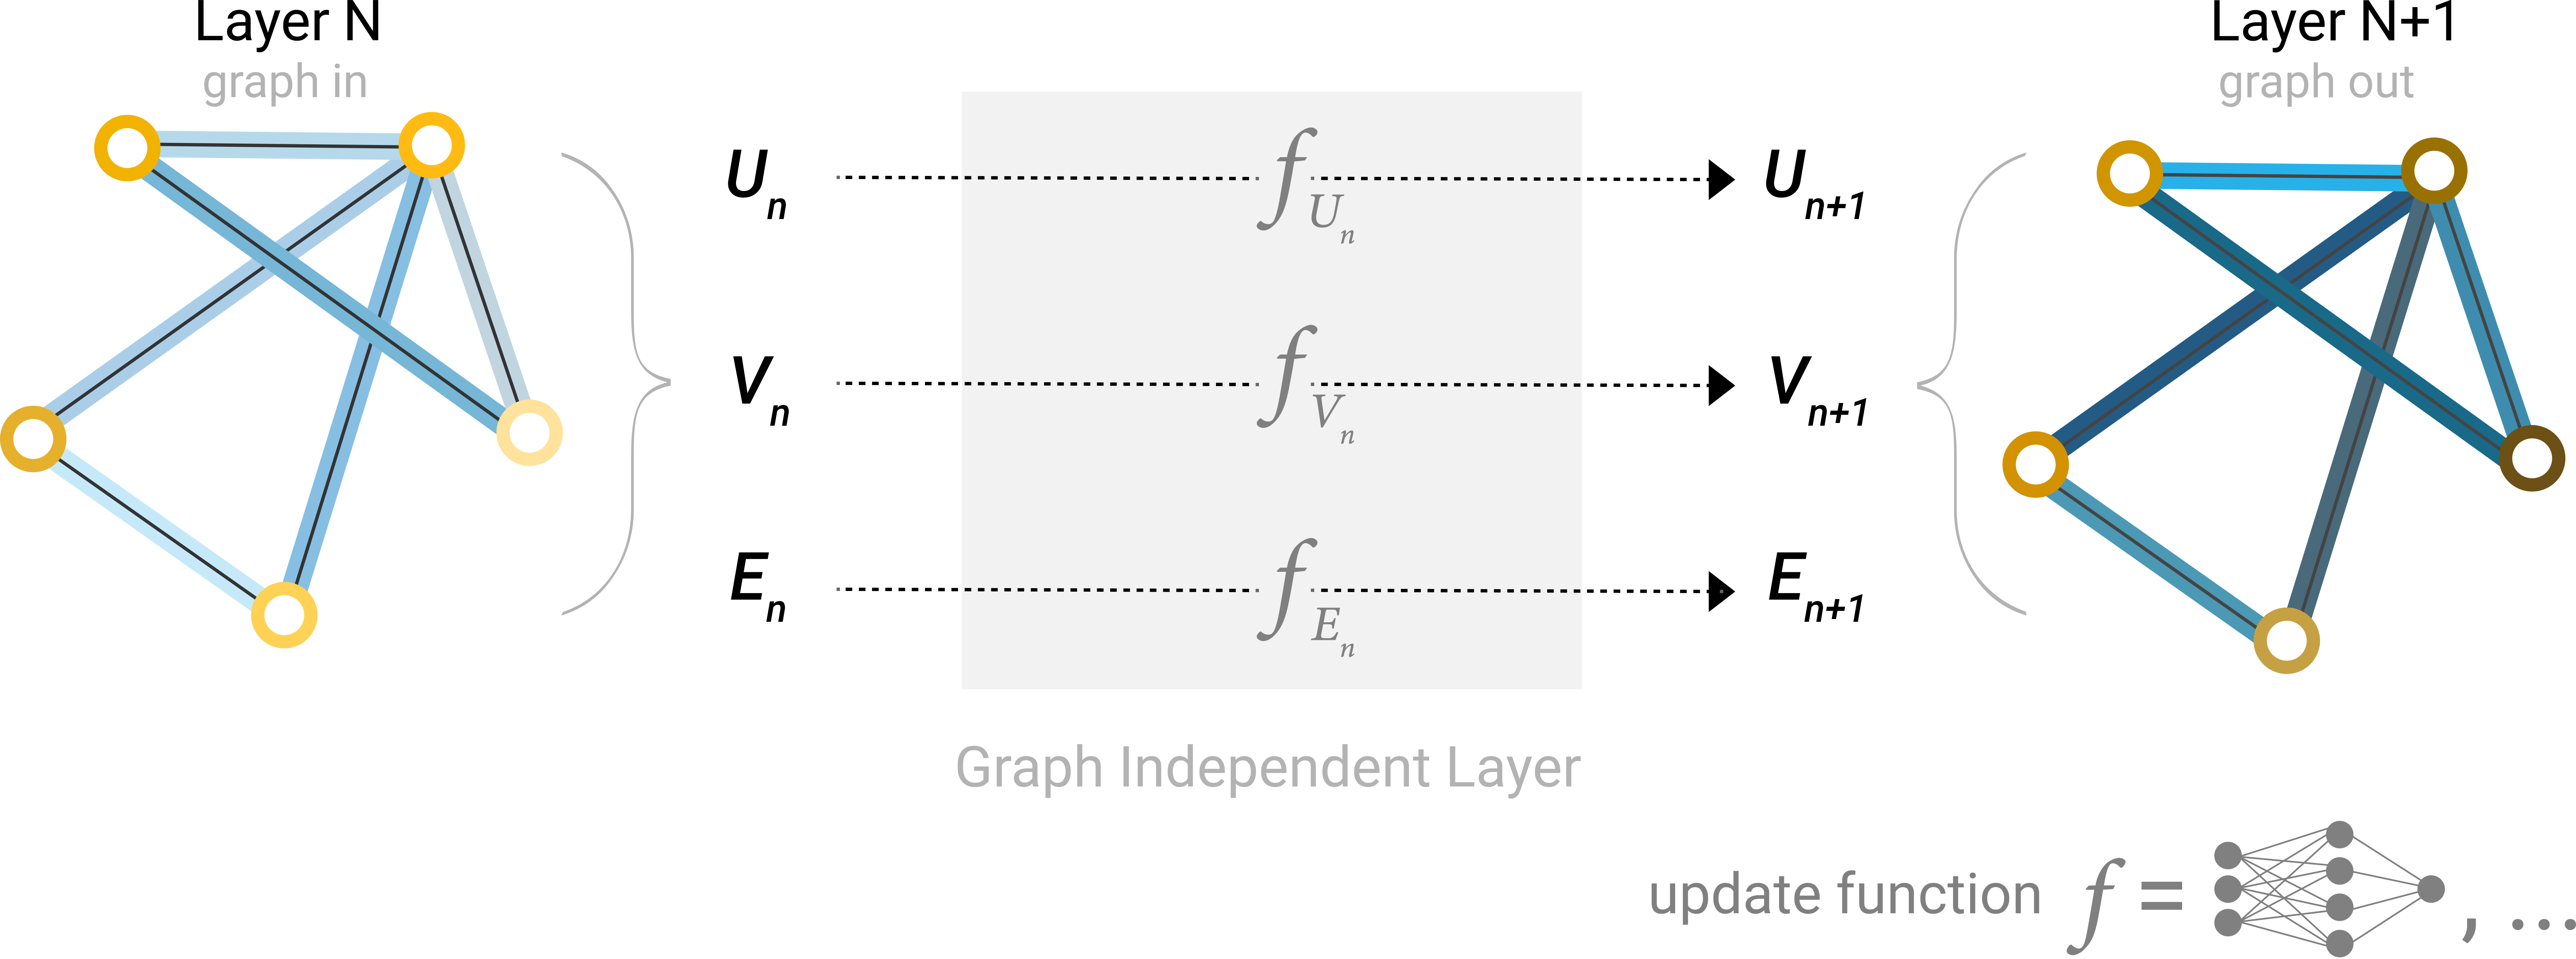
\includegraphics[width=\textwidth]{gnn-block.png}
	\caption{A simple \ac{GNN} block. At layer $N$, the current graph $(V_n, E_n, U_n)$ is updated to $(V_{n+1}, E_{n+1}, U_{n+1})$, in which $V_n$ is the list of feature vectors for nodes, $E_n$ is the list of feature vectors for edges, and $U_n$ is global value. The three \ac{MLP} are $f_{U_n}$, $f_{V_n}$, $f_{E_n}$ correspond to each mentioned graph attributes.}
	\label{fig:gnn-block}
\end{figure}

We of course can have multiple of these blocks, similarly to have multiple hidden layers in a \ac{MLP}.
\begin{figure}[hbt!]
	\centering
	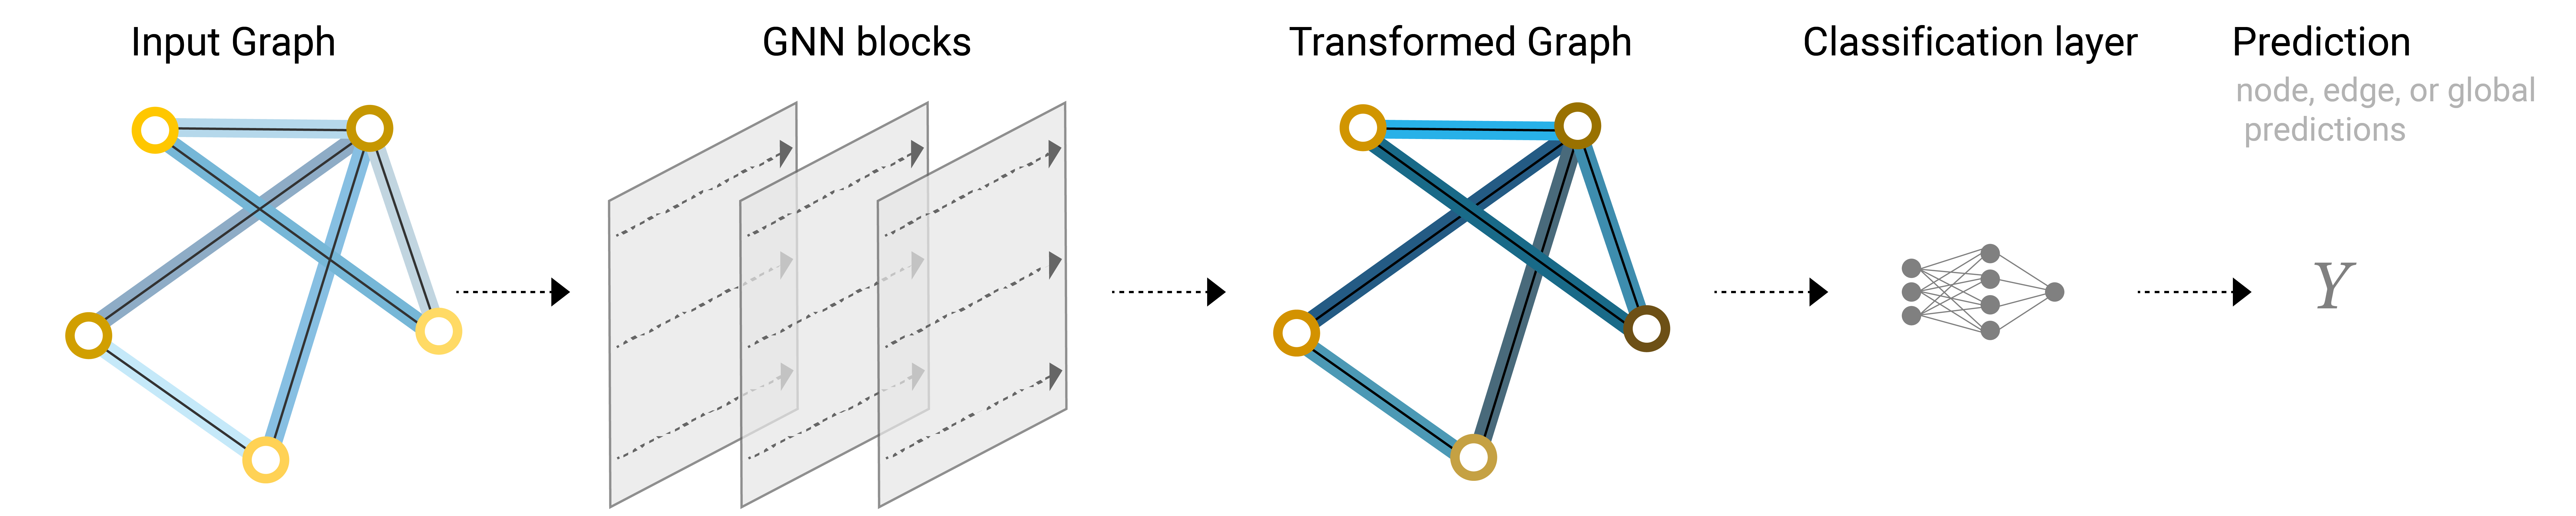
\includegraphics[width=\textwidth]{gnn-blocks.png}
	\caption{Multiple \ac{GNN} blocks before prediction network.}
	\label{fig:gnn-blocks}
\end{figure}

\subsection{GNN Predictions}
For specific prediction task, an additional \ac{MLP} operates with corresponding graph attribute.
\begin{figure}[hbt!]
	\centering
	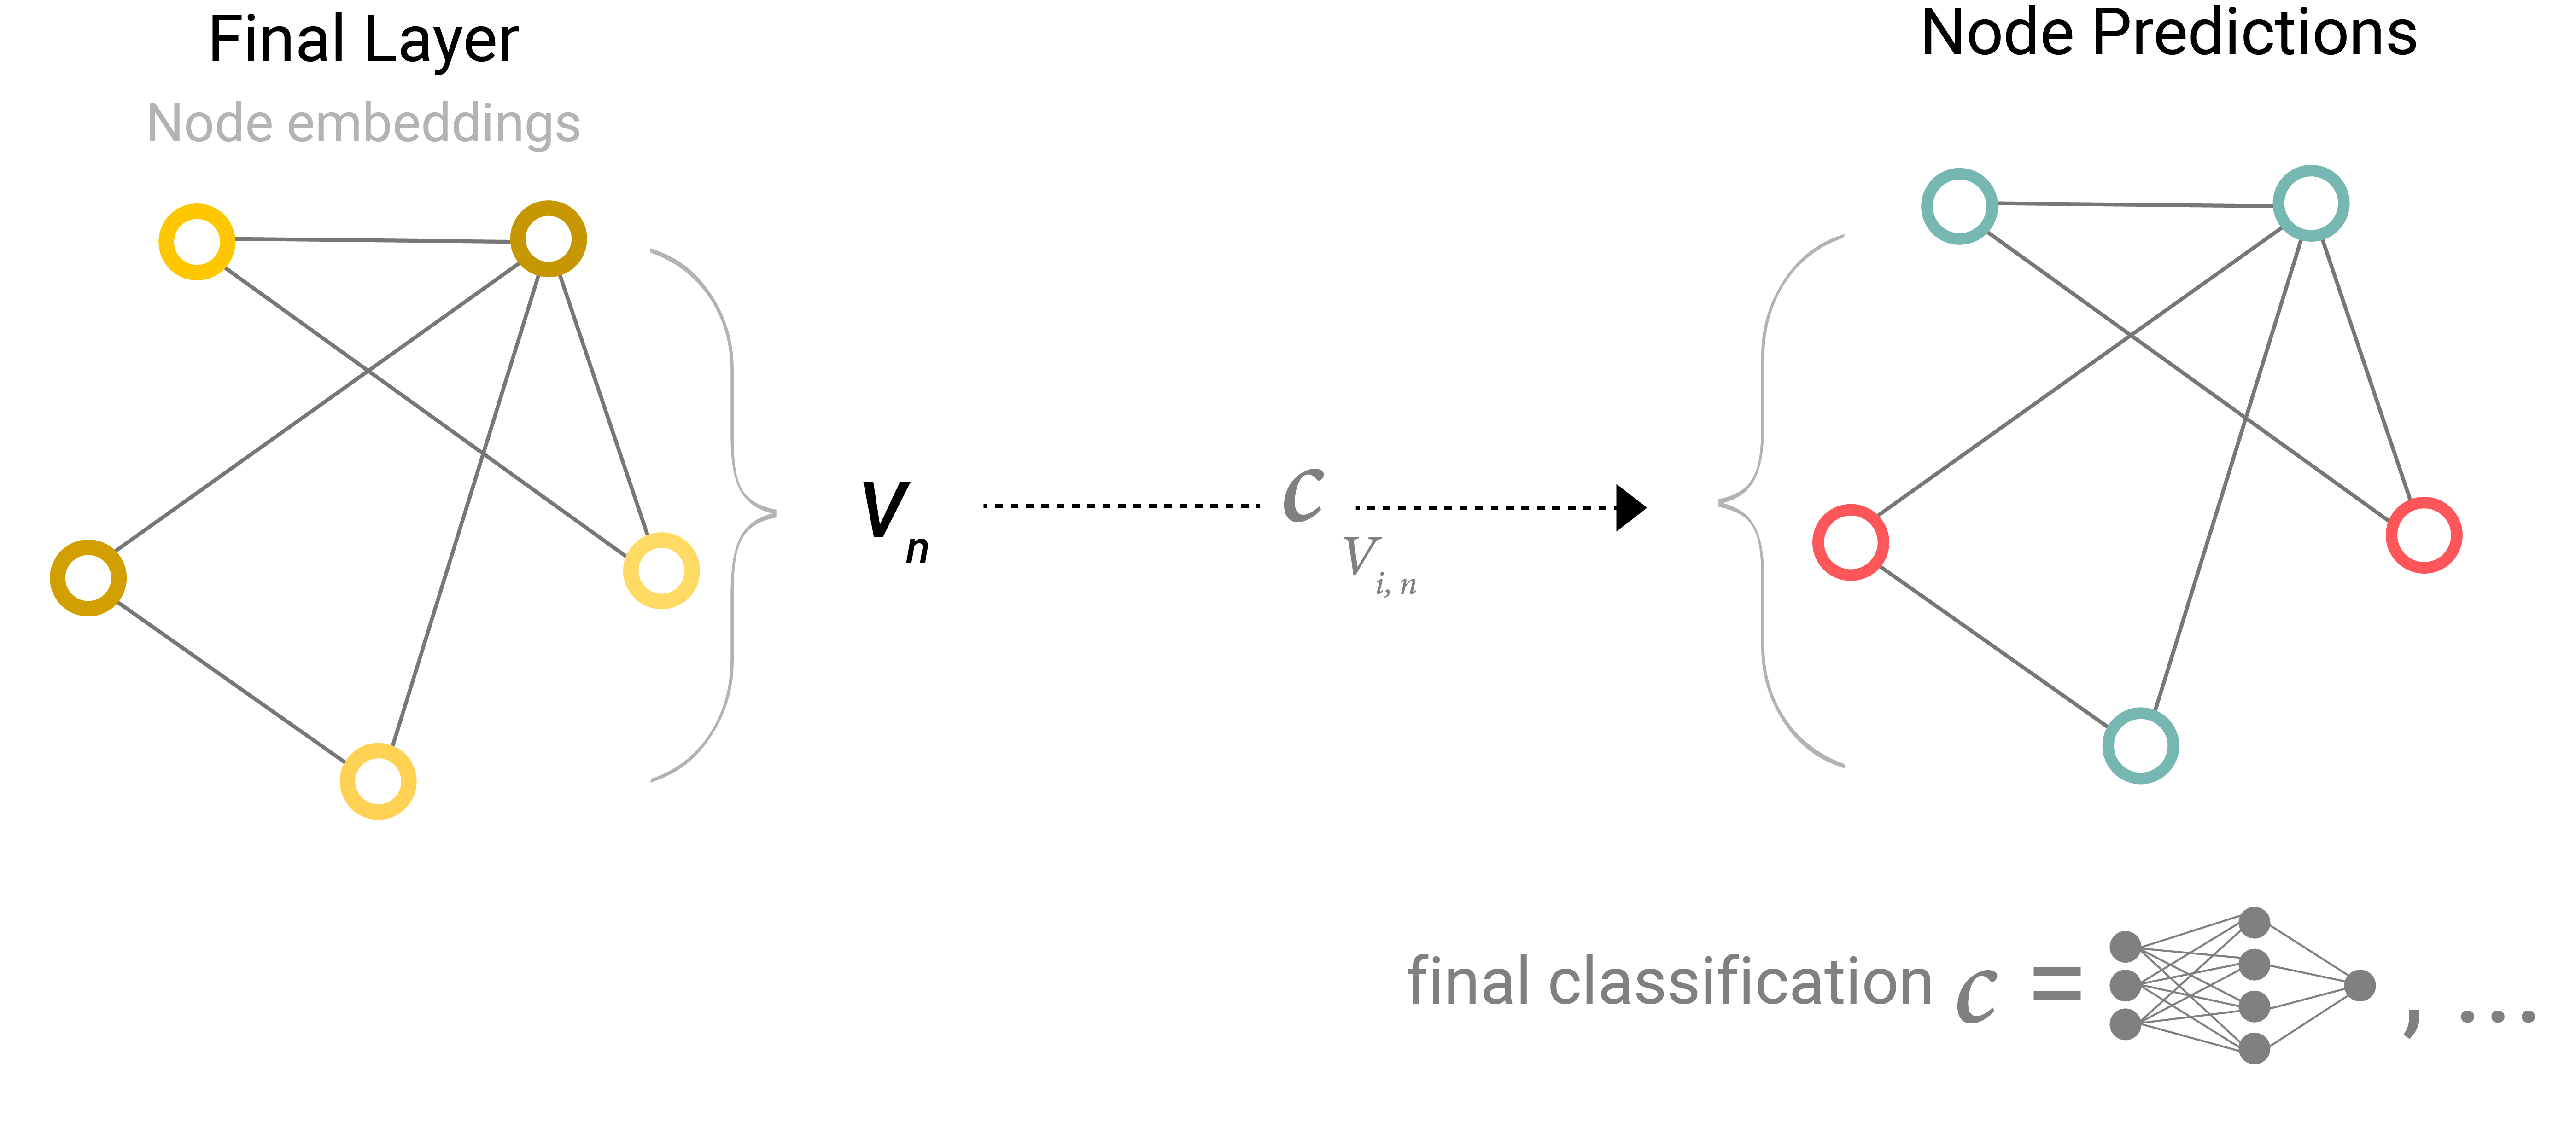
\includegraphics[width=\textwidth]{gnn-prediction.png}
	\caption{Example of node-level prediction task: A \ac{MLP} $C_{V_{i,n}}$ produces prediction score on each node.}
	\label{fig:gnn-prediction}
\end{figure}

\subsection{Pooling Information}
Information may not be sufficient and complete in graph
\begin{itemize}
	\item Having only edge-level features, need to make node-level predictions.
	\item Having only node-level features, need to make edge-level predictions.
\end{itemize}

In these cases, the information can be transfer via pooling operation:
\begin{enumerate}
	\item Embeddings are gathered and concatenate into a matrix.
	\item The output embedding are then aggregated from the matrix, usually via a sum operation (\figref{fig:gnn-pooling}).
\end{enumerate}
\begin{figure}[hbt!]
	\centering
	\begin{subfigure}[b]{0.47\textwidth}
		\centering
		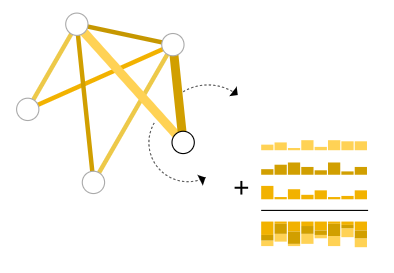
\includegraphics[width=\textwidth]{gnn-pooling.png}
	\end{subfigure}
	\hfill
	\begin{subfigure}[b]{0.47\textwidth}
		\centering
		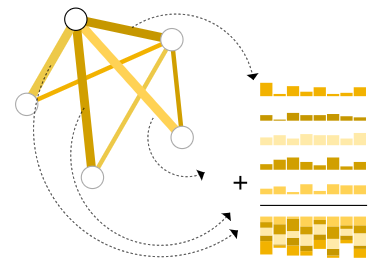
\includegraphics[width=\textwidth]{gnn-pooling-1.png}
	\end{subfigure}
	\caption{Example of pooling operation via sum. The feature embeddings of neighboring edges are aggregated to the node embedding, via a sum operation.}
	\label{fig:gnn-pooling}
\end{figure}
\begin{figure}[hbt!]
	\centering
	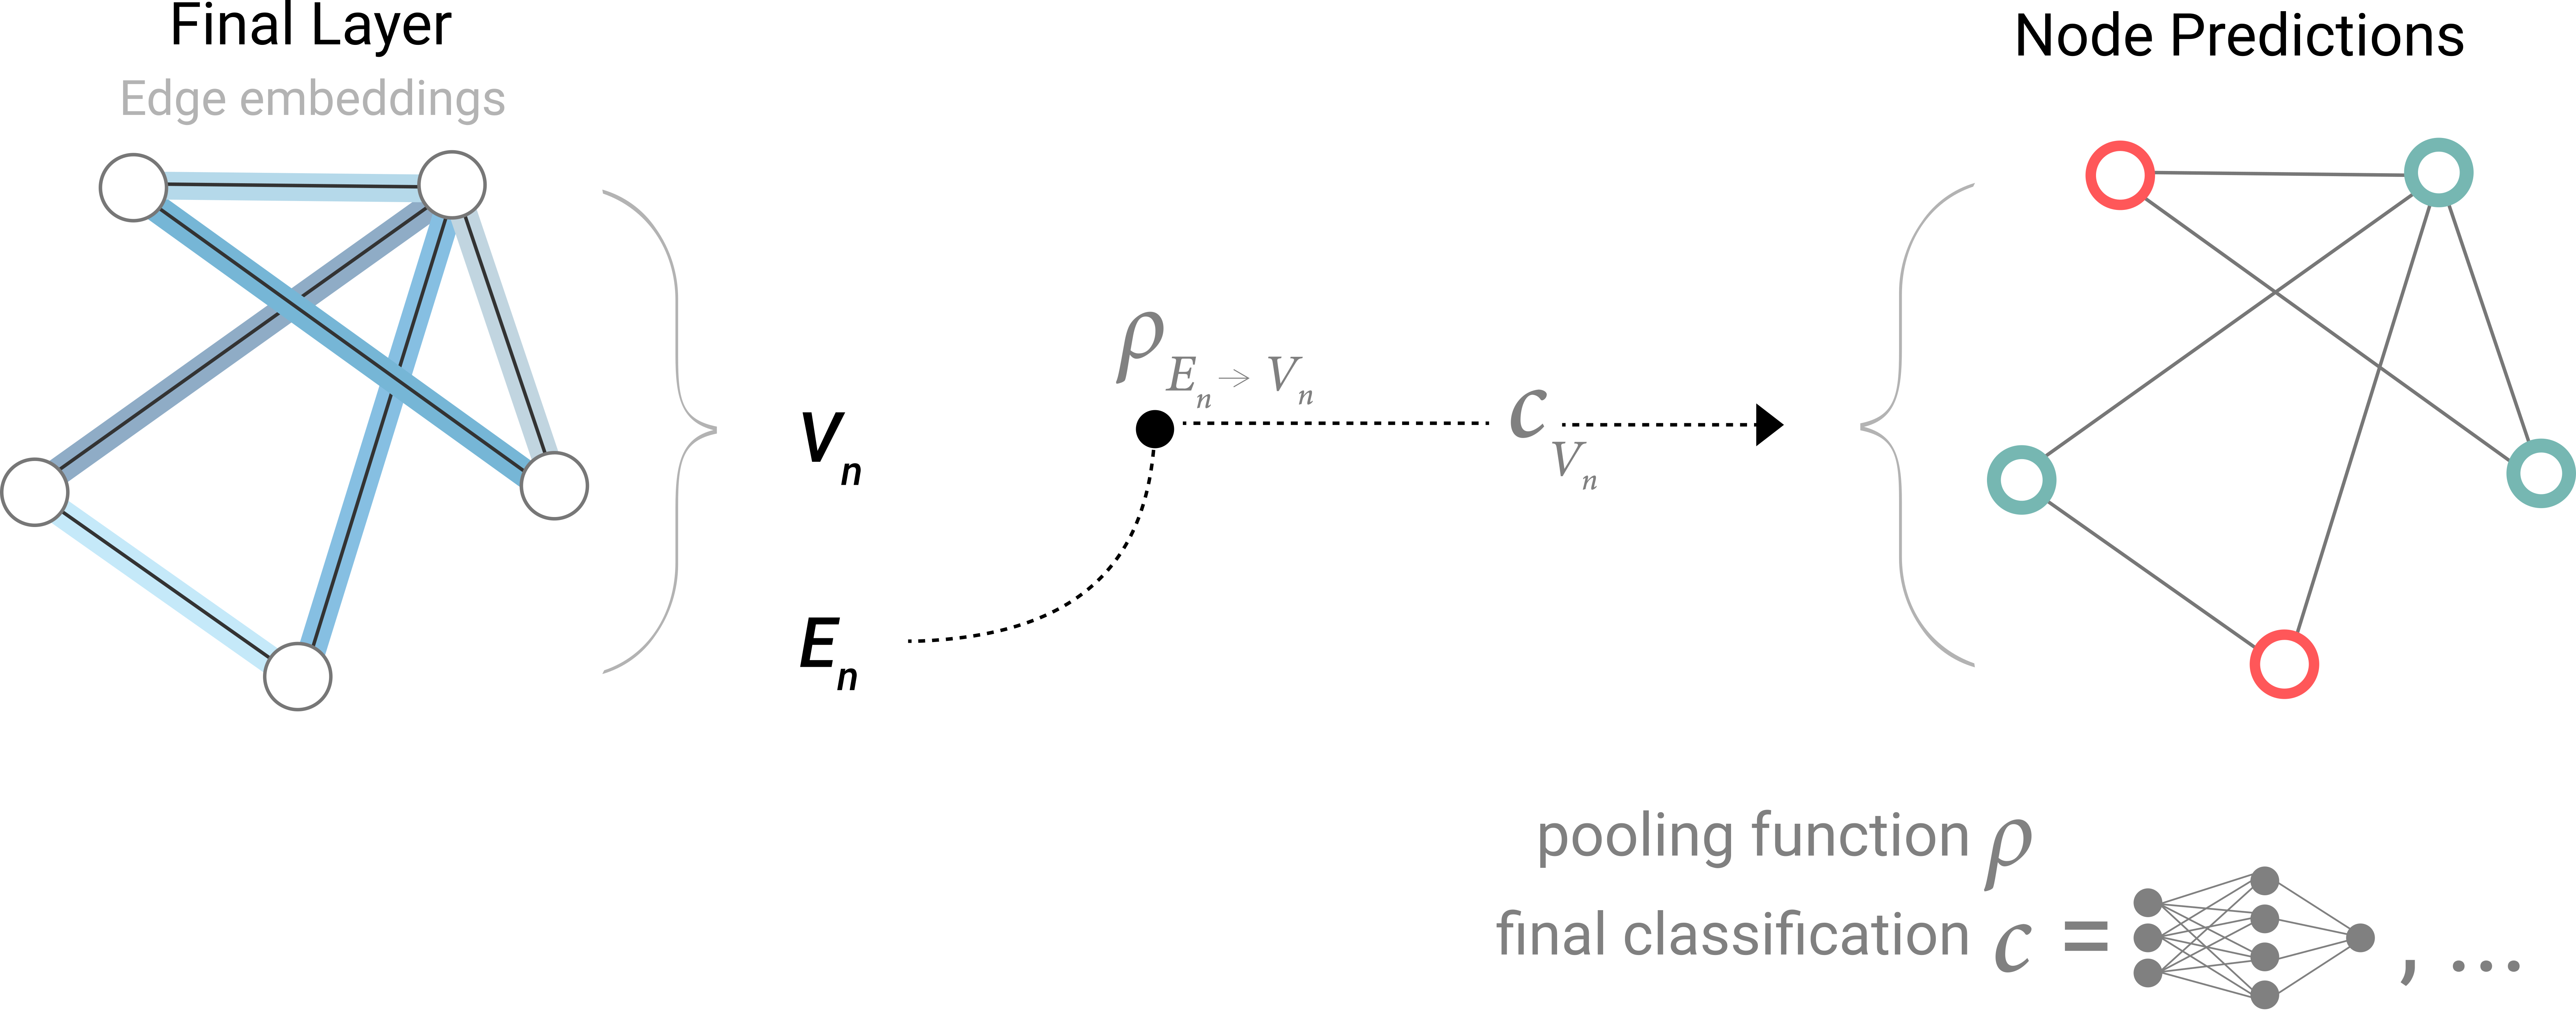
\includegraphics[width=\textwidth]{gnn-pooling-edge2node.png}
	\caption{Pooling operation from edge to node $\rho_{E_n \rightarrow V_n}$ before applying node-level prediction $C_{V_n}$.}
	\label{fig:gnn-pooling-edge2node}
\end{figure}

\subsection{Message Passing}
In \ac{GNN}, while pooling implies transferring information from one graph attribute to another (\eg, edge to node), message passing implies exchanging information and influence within the same graph attribute (\eg, node to node). The procedure, however, is similar to pooling.
\begin{figure}[hbt!]
	\centering
	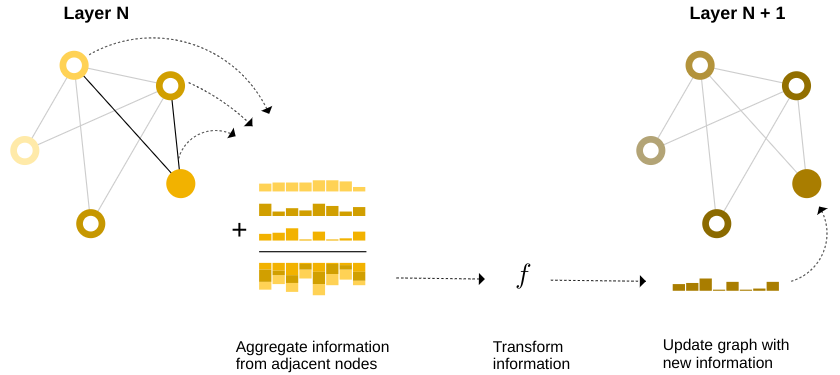
\includegraphics[width=\textwidth]{gnn-message-passing.png}
	\caption{Message passing in graph: $\rho_{V_n \rightarrow V_{n+1}}$}
	\label{fig:gnn-message-passing}
\end{figure}

Combining different embeddings from different graph attributes can all be considered as a conditioning function:
\begin{figure}[hbt!]
	\centering
	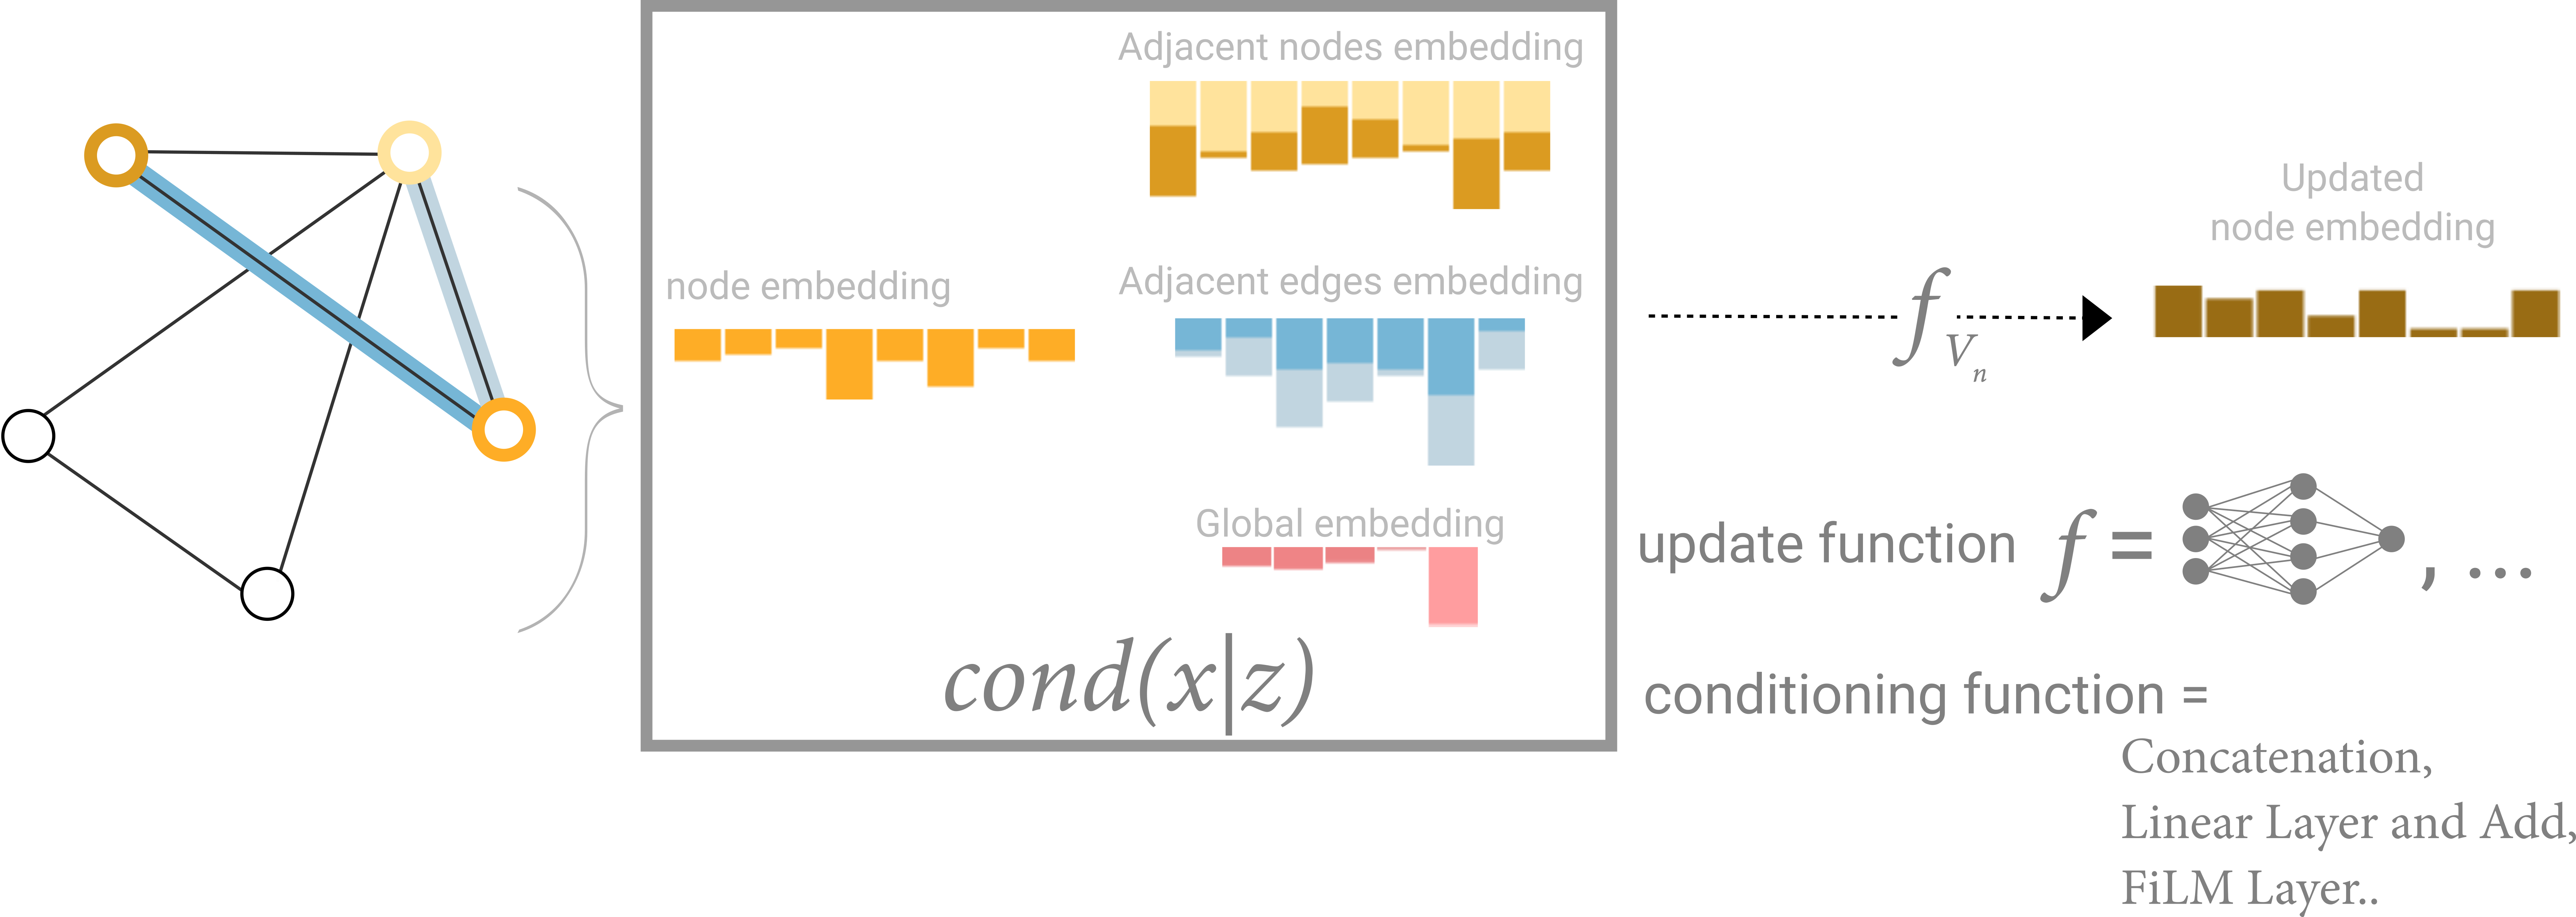
\includegraphics[width=\textwidth]{gnn-conditioning.png}
	\caption{Schematic for conditioning one node's embedding based on three other embeddings (adjacent nodes, adjacent edges, global).}
	\label{fig:gnn-conditioning}
\end{figure}

\begin{figure}[hbt!]
	\centering
	\begin{minipage}{.47\textwidth}
		\centering
		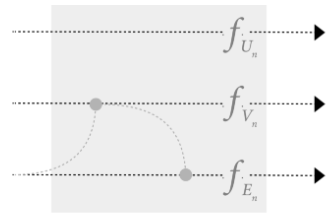
\includegraphics[width=.6\textwidth]{gnn-node-edge-learning.png}
		\captionof{figure}{Node then edge learning}
	\end{minipage}
	\hfil
	\begin{minipage}{.47\textwidth}
		\centering
		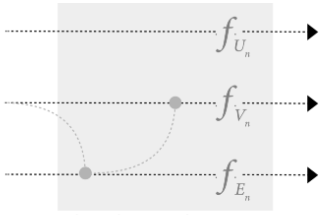
\includegraphics[width=.6\textwidth]{gnn-edge-node-learning.png}
		\captionof{figure}{Edge then node learning}
	\end{minipage}
\end{figure}
\begin{figure}[hbt!]
	\centering
	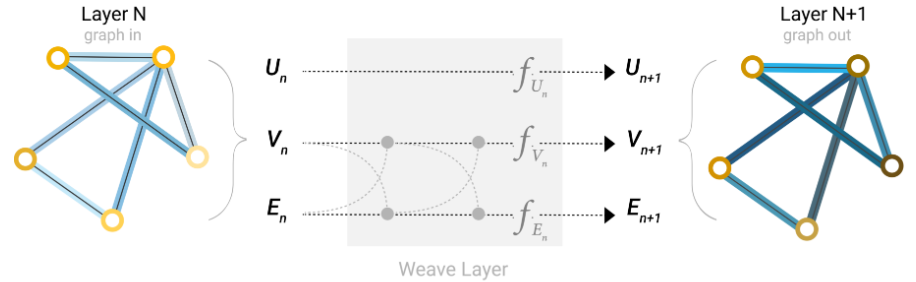
\includegraphics[width=.9\textwidth]{gnn-weave.png}
	\caption{Learning in "weave fashion".}
\end{figure}
\begin{figure}[hbt!]
	\centering
	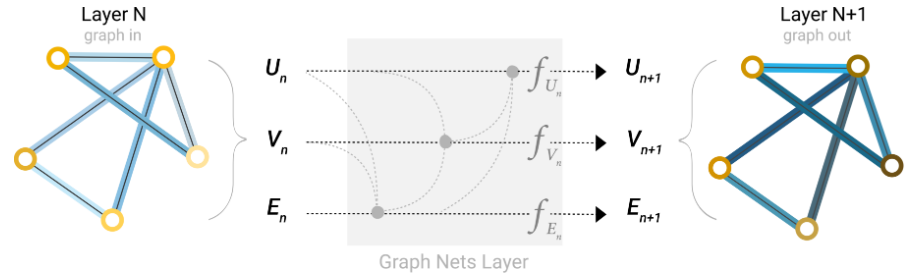
\includegraphics[width=.9\textwidth]{gnn-graph-net.png}
	\caption{Schematic of a Graph Nets architecture leveraging global representations.}
\end{figure}

\subsection{Some Empirical Design Lessons}
Source: \citeaustitle{sanchez2021a}
\begin{itemize}
	\item A higher number of parameters does correlate with higher performance.
	\item \ac{GNN}s are a very parameter-efficient model type: for even a small number of parameters
	\item Models with higher dimensionality or more layers tend to have better mean and lower bound performance, but the same trend is not found for the maximum.
	\item \ac{GNN} with a higher number of layers will broadcast information at a higher distance and can risk having their node representations ‘diluted’ from many successive iterations
	\item Sum has a very slight improvement on the mean performance, but max or mean can give equally good models.
	\item The more type of message passing the model has, the better the performance is.
\end{itemize}

\subsection{Application}
Source: \href{https://youtu.be/p2aqXKfRXEA}{CS224W}
\begin{itemize}
	\item PinSAGE: \ac{GNN} for Recommendation systems: nodes are users, products. Based on other users' interactions with some products, predict whether one user would interest in a new product.
	\item Decagon: heterogeneous \ac{GNN} for drug prediction
	\item Goal-directed generation: GCPN for molecule generation
\end{itemize}

\subsection{References}
\begin{itemize}
	\item \href{https://youtu.be/bA261BF0bdk}{Siraj Raval YouTube}
	\item \citeaustitle{sanchez2021a}
	\item \citeaustitle{daigavane2021understanding}
	\item \citeaustitle{gordic2021how}
\end{itemize}

There are so many current open problems for research (2022)
\begin{itemize}
	\item Convolutions on Graphs \cite{daigavane2021understanding}
	\item Multi-graphs
	\item Hyper-graphs
	\item Hyper-nodes
	\item hierarchical graphs
	\item Graph convolutions
	\item Graph Attention Networks
	\item Generative modeling
\end{itemize}
\include{Contents/word-embeddings.tex}
% !TeX spellcheck = en_US
\chapter{Generative Models}

\section{Basics Definitions}
Check \secref{sec:vae-defs}
\begin{itemize}
	\item Generative models: are models that generate data $x$. \Eg: $p(x)$ is a generative model, because knowing $p(x)$, we can sample $x$.
\end{itemize}

\note
\begin{itemize}
	\item Not all generative models are not necessary latent variable models, and not all latent variable models are generative models. But it's common for a generative model to be a latent variable model, because sometimes, to generate data, we usually want to know the \ac{prob} distribution of it. When that \ac{prob} distribution is complex, we would represent it as a product of multiple simple \ac{prob} distribution, using some latent variables.
\end{itemize}

% !TeX spellcheck = en_US
\chapter{Hyperparameters Optimization}

\section{Introduction}
Hyperparameters are \ac{param} that:
\begin{itemize}
	\item Define model's architecture
	\item Do NOT change with your model training
	\item Are NOT learnt from your model training
	\item Each model has its own set of \ac{param}
\end{itemize}

Hyperparameters tuning affects:
\begin{itemize}
	\item Speed of convergence
	\item Generalization of your model
	\item Find optimal solution space
	\item Find right capacity for your solution
	\item Identify ideal architecture
\end{itemize}

Examples:
\begin{itemize}
	\item Different types of gradient descents
	\item \dots
\end{itemize}

\section{Exhaustive Search}
\subsection{Grid Search}
Grid search will suffer to the curse of dimensionality
\begin{itemize}
	\item Define range of possible values for all \ac{param}
	\item Evaluate model performance for each hyper\ac{param} combination
	\item Cross validate
	\item Pick the top $N$ hyper\ac{param}
\end{itemize}

\subsection{Random Search}
Random search is generally faster and more efficient, though does NOT guarantee good coverage.
\begin{itemize}
	\item Define random sampling space (explicit values or distribution)
	\item Sample hyper\ac{param} randomly
	\item Evaluate model performance for each hyper\ac{param} combination
	\item Cross validate
	\item Pick the top $N$ hyper\ac{param}
\end{itemize}

\subsection{Example}
Python libraries:
\begin{python}
from sklearn.model_selection import GridSearchCV
from sklearn.model_selection import RandomizedSearchCV
\end{python}

Examples:
\begin{itemize}
	\item \href{https://youtu.be/HdlDYng8g9s}{codebasics YouTube}
\end{itemize}

\section{Sequential Model Based}
\subsection{Bayesian Optimization}
Use Acquisition function \todo{}
\subsection{Genetic Algorithm}
\todo{}

\begin{python}
from skopt import BayesSearchCV
\end{python}

\section{Tools}
Current good tools for hyper\ac{param} search:
\begin{itemize}
	\item Weights \& Biases: \pyth{import wandb}
	\item Scikit-learn: \pyth{from sklearn.model_selection import *}
	\item SkOpt: \pyth{skopt}
\end{itemize}

\section{References}
\begin{itemize}
	\item \href{https://youtu.be/ttE0F7fghfk}{Siraj Raval YouTube}
	\item \href{https://www.youtube.com/channel/UCS1dQr2X_ComHN4PXYDS4gA}{Machine Learning Mastery YouTube}
\end{itemize}
% !TeX spellcheck = en_US
\chapter{Deep Learning Generalization}
This chapter presents different techniques and idea to generalize deep learning and make it more applicable to variety of problems.

\section{Transfer Learning}
Transfer learning focuses on storing knowledge gained while solving a problem and applying it to a different but related problem. Simply put:
\begin{itemize}
	\item The new model comprises mostly of layers from a pretrained model.
	\item We take the structure and corresponding \ac{param} of a model that is pretrained on a large dataset for the feature extraction.
	\item We add a few (1-2) new layers in the end, which are designated to our current specific problem.
\end{itemize}


\note
\begin{itemize}
	\item Lower the learning rate
\end{itemize}

Example with \texttt{TensorFlow} (\href{https://github.com/codebasics/deep-learning-keras-tf-tutorial/tree/master/18_transfer_learning}{src}):
\begin{python}
import tensorflow as tf
import tensorflow_hub as hub

model_path = "https://tfhub.dev/google/tf2-preview/mobilenet_v2/feature_vector/4"
pretrained_model = hub.KerasLayer(
		model_path, input_shape=(224, 224, 3), trainable=False)

num_of_new_classes = 5
model = tf.keras.Sequential([
		pretrained_model,
		tf.keras.layers.Dense(num_of_new_classes)])
model.summary()

model.compile(
		optimizer="adam",
		loss=tf.keras.losses.SparseCategoricalCrossentropy(from_logits=True),
		metrics=['acc'])

model.fit(X_train_scaled, y_train, epochs=5)
\end{python}

\section{Fine-Tuning}
In fine-tuning, a pretrained model is used, just like in transfer learning.
\begin{itemize}
	\item In fine-tuning, we retrain the whole model with the new dataset, while in transfer learning, we freeze the \ac{param} of pretrained model.
	\item Can incrementally adapt the pretrained features to the new dataset
\end{itemize}

\section{Distillation}
\todo{Knowledge distillation, model distillation, dataset distillation}
\section{Meta-Learning}
\section{Multi-task Learning}

\section{References}
% !TeX spellcheck = en_US
\chapter{Technical Tools}

This chapter talks about or at least lists out helpful tools, platforms for using/working with \ac{DL} and \ac{ML} in general.

\section{Supporting Platforms \& Tools}
\begin{itemize}
	\item \href{https://github.com/fastai/fastai}{fastai}: simplifies training fast and accurate neural nets using modern best practices
	\item \href{https://wandb.ai/site}{Weights and Biases}: builds better models faster with experiment tracking, dataset versioning, and model management	
\end{itemize}

\section{Coding Libraries}
Libraries for generic \ac{ML}:
\begin{itemize}
	\item \href{https://scikit-learn.org/stable/}{scikit-learn} is a free software \ac{ML} library for the Python programming language
	\item \href{https://xgboost.ai/}{XGBoost}: Scalable and Flexible Gradient Boosting
\end{itemize}

Libraries for building \ac{DL} models:
\begin{itemize}
	\item \href{https://keras.io/}{Keras}: is an open-source software library that provides a Python interface for artificial neural networks. Keras acts as an interface for the TensorFlow library.
\begin{python}
	from tensorflow import keras
	from tensorflow.keras import layers
\end{python}
	\item \href{https://www.tensorflow.org/overview}{TensorFlow}: is an end-to-end open source platform for \ac{ML}
\begin{python}
	import tensorflow as tf
	print("TensorFlow version:", tf.__version__)
\end{python}
	\item \href{https://pytorch.org/}{PyTorch}: is an open source \ac{ML} framework that accelerates the path from research prototyping to production deployment.
\begin{python}
	import torch
	from torch import nn
	from torch.utils.data import DataLoader
	from torchvision import datasets
\end{python}
	\item Sonnet: DeepMind's library for constructing neural networks in TensorFlow. Check this \href{https://youtu.be/rlpQjnUvoKw}{YouTube video}. It can be seen as a library to make TensorFlow more suitable for research purposes at DeepMind.
\begin{python}
	$ pip install dm-sonnet
	import sonnet as snt
	import tensorflow as tf
\end{python}
\end{itemize}

Comparisons on \href{https://www.assemblyai.com/blog/pytorch-vs-tensorflow-in-2022/}{assemblyai.com}, \href{https://towardsdatascience.com/pytorch-vs-tensorflow-spotting-the-difference-25c75777377b}{towardsdatascience.com}, \href{https://builtin.com/data-science/pytorch-vs-tensorflow}{builtin.com}: \tabref{tab:tensorflow-vs-pytorch}
\begin{table}[hbt!]
	\centering
	\begin{tabular}{m{7.9cm}|m{7.9cm}}
		TensorFlow (Google) & PyTorch (Facebook)\\ \hline\hline
		Static graph definition & Dynamic graph definition: \newline you can define, change and execute nodes as you go, no special session interfaces or placeholders.\\ \hline
		Awesome Tensorboard's visualization &\\ \hline
		Better deployment with \href{https://www.tensorflow.org/tfx/guide/serving}{TensorFlow Serving} & \\ \hline
		\href{https://www.tensorflow.org/guide/distributed_training}{Distributed model training} & \\ \hline
		Data parallelism require more manual work and careful thought & Easy Declarative data parallelism\\ \hline
		& more clear and developer-friendly
	\end{tabular}
	\caption{Comparison between TensorFlow and PyTorch.}
	\label{tab:tensorflow-vs-pytorch}
\end{table}

Guide on choosing which library to work with:
\begin{itemize}
	\item If you are in the industry: \figref{fig:pytorch-vs-tensorflow}
	\item If you are a researcher: \figref{fig:pytorch-vs-tensorflow-1}
\end{itemize}
\begin{figure}[hbt!]
	\centering
	\begin{subfigure}[b]{0.49\textwidth}
		\centering
		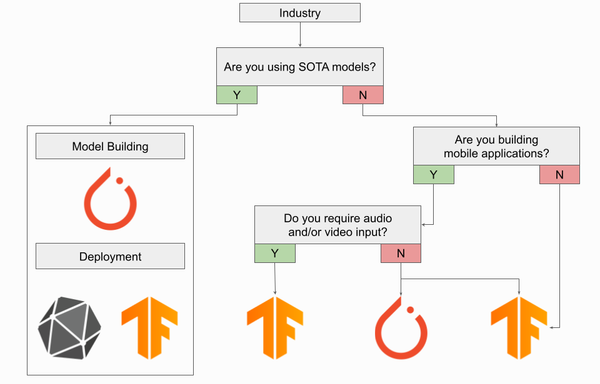
\includegraphics[width=\textwidth]{pytorch-vs-tensorflow.png}
		\caption{If I’m in Industry}
		\label{fig:pytorch-vs-tensorflow}
	\end{subfigure}
	\hfill
	\begin{subfigure}[b]{0.49\textwidth}
		\centering
		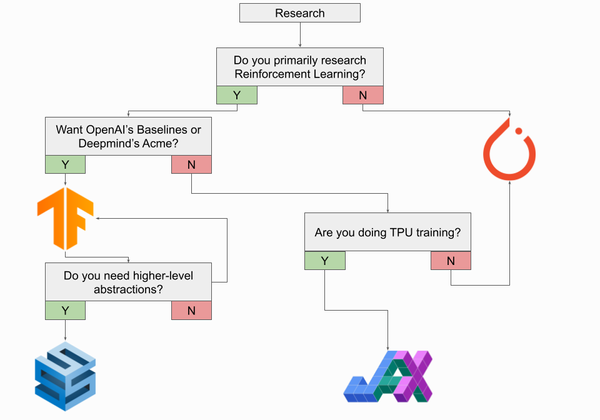
\includegraphics[width=\textwidth]{pytorch-vs-tensorflow-1.png}
		\caption{If I’m a Researcher}
		\label{fig:pytorch-vs-tensorflow-1}
	\end{subfigure}
	\caption{Choosing \ac{DL} libraries to work with \cite{cornor2021}.}
\end{figure}

\section{Cloud GPU Platforms}
\ac{DL} takes an extensive amount of time for training and computation tasks. \ac{GPU}s are designed to solve this problem. They offer high efficiency to perform heavy computations and faster training for your \ac{AI} models in parallel. According to Indigo research, \ac{GPU}s can offer \hlb{250 times faster} performance than \ac{CPU}s while training neural networks associated with deep learning. \cite{pathak2022}

Benefits of using Cloud \ac{GPU}s are:
\begin{itemize}
	\item Highly scalable
	\item Cost minimization
	\item Clearance of local resources
	\item Time saving
\end{itemize}

Cloud GPU Platforms for \ac{AI} and Massive Workload:
\begin{itemize}
	\item \href{https://cloud.google.com/compute/docs/gpus}{Google Cloud \ac{GPU}s}
	\item \href{https://www.ibm.com/cloud/gpu}{IBM Cloud}
	\item AWS and NVIDIA
	\item Microsoft Azure and their Deep Learning Virtual Machine (DLVM). Check this \href{https://medium.com/@manikantayadunanda/setting-up-deeplearning-machine-and-fast-ai-on-azure-a22eb6bd6429}{guide}
	\item \href{https://lambdalabs.com/service/gpu-cloud}{Lambda GPU}
	\item \href{https://www.paperspace.com/core}{Paperspace CORE}
	\item Others worth mentioned: Linode, Elastic \ac{GPU} service, OVHcloud, Genesis Cloud
\end{itemize}

For comparisons between services:
\begin{itemize}
	\item \url{https://cloud-gpus.com/}
	\item \url{https://www.paperspace.com/gpu-cloud-comparison}
	\item \url{https://www.dataversity.net/cloud-gpu-instances-what-are-the-options/}
\end{itemize}

\section{Distributed Learning}
\textit{Distributed Learning}, \ac{aka} \textit{distributed training}, is the problem of how you couple the training process given multiple \ac{GPU}s.

\begin{itemize}
	\item Data Parallelism: \figref{fig:data-parallelism}. The training could be synchronous or asynchronous
	\item Model Parallelism: \figref{fig:model-parallelism}
\end{itemize}

\begin{figure}[hbt!]
	\centering
	\begin{subfigure}[b]{0.4\textwidth}
		\centering
		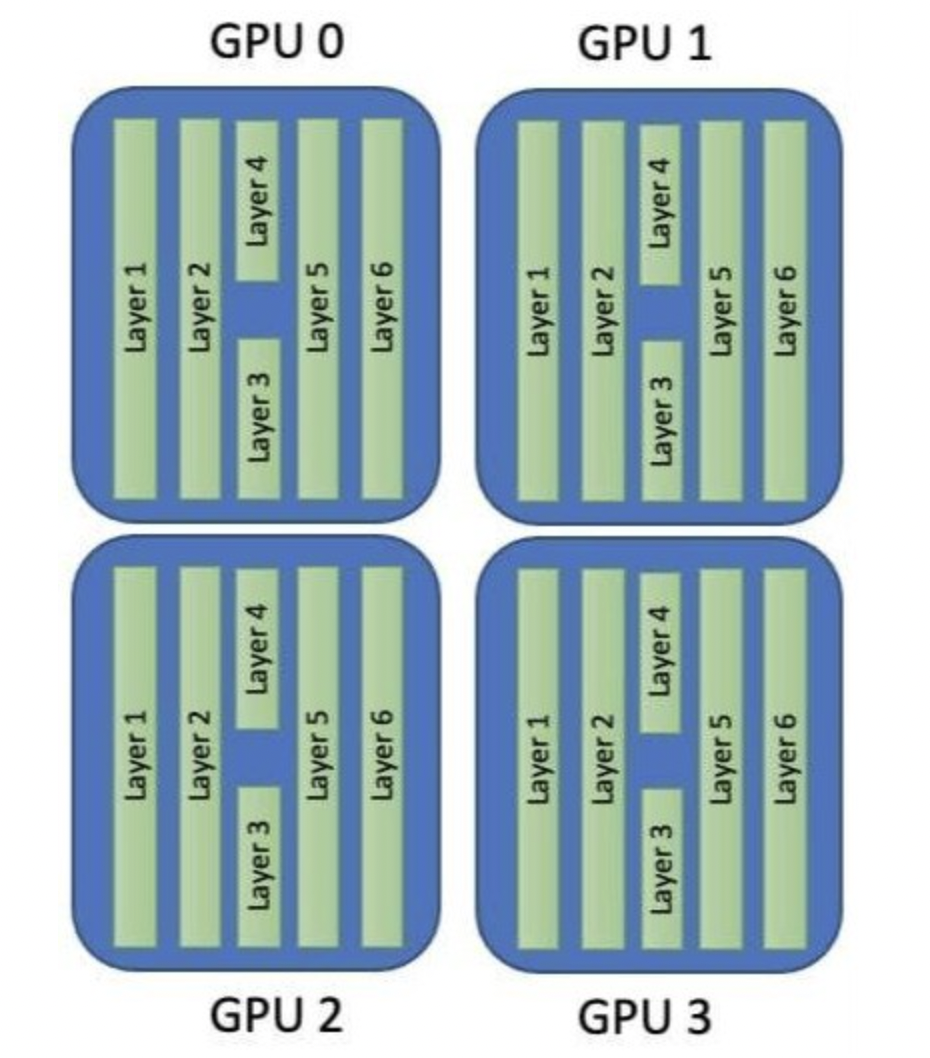
\includegraphics[width=\textwidth]{data-parallelism.png}
		\caption{Data parallelism.}
		\label{fig:data-parallelism}
	\end{subfigure}
	\hfill
	\begin{subfigure}[b]{0.45\textwidth}
		\centering
		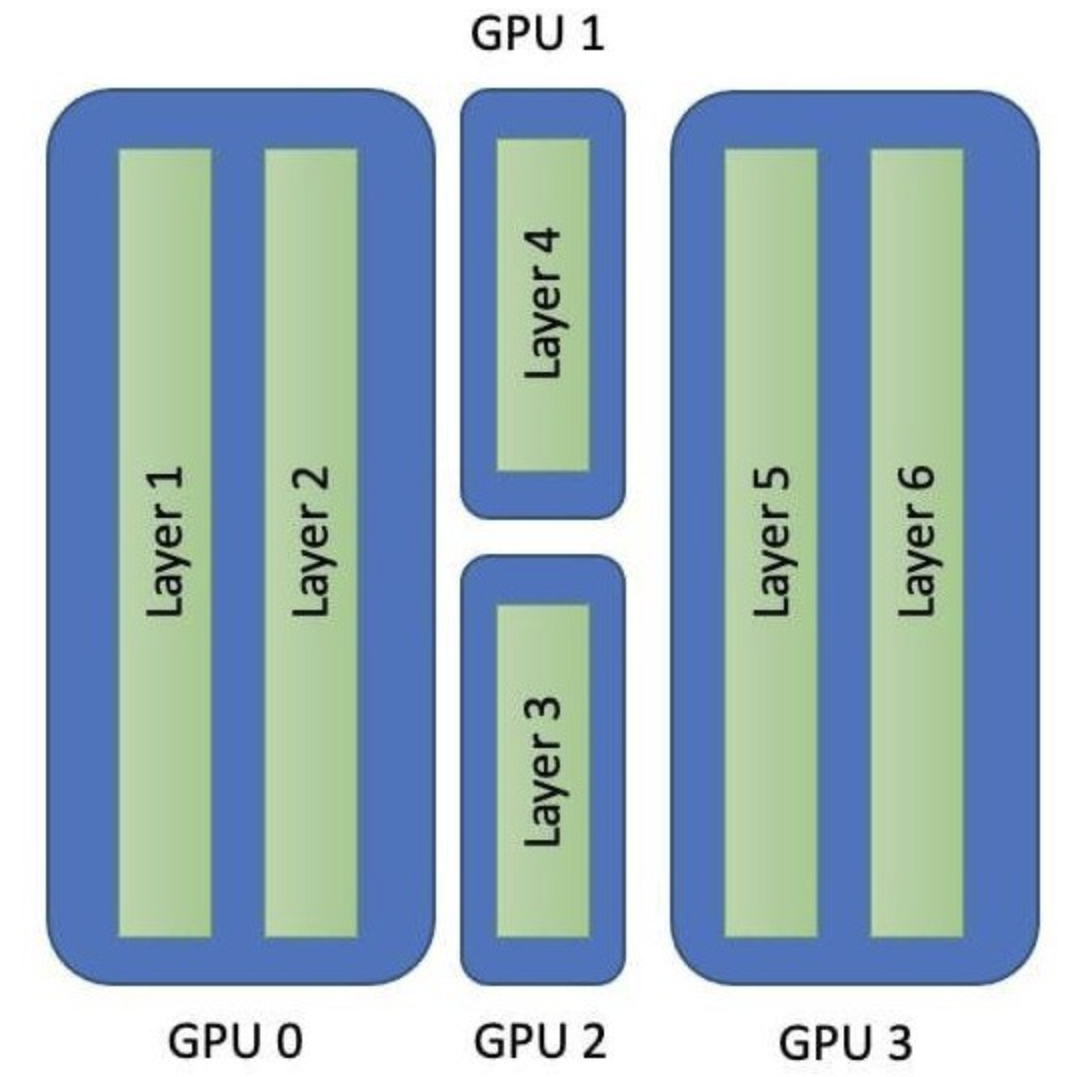
\includegraphics[width=\textwidth]{model-parallelism.png}
		\caption{Model parallelism.}
		\label{fig:model-parallelism}
	\end{subfigure}
	\caption{Deep Learning on Supercomputers (\href{https://towardsdatascience.com/deep-learning-on-supercomputers-96319056c61f}{src}).}
\end{figure}

\subsection{Example}
\texttt{TensorFlow} example for data parallelism (\href{https://github.com/codebasics/deep-learning-keras-tf-tutorial/tree/master/43_distributed_training}{src}):
\begin{python}
import os
os.environ["CUDA_VISIBLE_DEVICES"]="4"

import tensorflow as tf
from tensorflow import keras

tf.config.experimental.list_physical_devices()
tf.test.is_built_with_cuda()

# Create model
...

strategy = tf.distribute.MirroredStrategy()
strategy.num_replicas_in_sync

# Training with CPU
with tf.device('/CPU:0'):
	cpu_model = get_model()
	cpu_model.fit(train_dataset, epochs=50)
	
# Training with GPU
with strategy.scope():
	gpu_model = get_model()
	gpu_model.fit(train_dataset, epochs=50)
\end{python}

\texttt{PyTorch} example for data parallelism (\href{https://pytorch.org/tutorials/beginner/blitz/data_parallel_tutorial.html}{src}):
\begin{python}
model = Model(input_size, output_size)
if torch.cuda.device_count() > 1:
	print("Using", torch.cuda.device_count(), "GPUs!")
	model = nn.DataParallel(model)
	
model.to(device)
\end{python}

\backmatter
\pagenumbering{Roman}
\printbibliography[heading=bibintoc]
\appendix
\end{document}